\documentclass[twoside]{book}

% Packages required by doxygen
\usepackage{fixltx2e}
\usepackage{calc}
\usepackage{doxygen}
\usepackage[export]{adjustbox} % also loads graphicx
\usepackage{graphicx}
\usepackage[utf8]{inputenc}
\usepackage{makeidx}
\usepackage{multicol}
\usepackage{multirow}
\PassOptionsToPackage{warn}{textcomp}
\usepackage{textcomp}
\usepackage[nointegrals]{wasysym}
\usepackage[table]{xcolor}

% Font selection
\usepackage[T1]{fontenc}
\usepackage[scaled=.90]{helvet}
\usepackage{courier}
\usepackage{amssymb}
\usepackage{sectsty}
\renewcommand{\familydefault}{\sfdefault}
\allsectionsfont{%
  \fontseries{bc}\selectfont%
  \color{darkgray}%
}
\renewcommand{\DoxyLabelFont}{%
  \fontseries{bc}\selectfont%
  \color{darkgray}%
}
\newcommand{\+}{\discretionary{\mbox{\scriptsize$\hookleftarrow$}}{}{}}

% Page & text layout
\usepackage{geometry}
\geometry{%
  a4paper,%
  top=2.5cm,%
  bottom=2.5cm,%
  left=2.5cm,%
  right=2.5cm%
}
\tolerance=750
\hfuzz=15pt
\hbadness=750
\setlength{\emergencystretch}{15pt}
\setlength{\parindent}{0cm}
\setlength{\parskip}{3ex plus 2ex minus 2ex}
\makeatletter
\renewcommand{\paragraph}{%
  \@startsection{paragraph}{4}{0ex}{-1.0ex}{1.0ex}{%
    \normalfont\normalsize\bfseries\SS@parafont%
  }%
}
\renewcommand{\subparagraph}{%
  \@startsection{subparagraph}{5}{0ex}{-1.0ex}{1.0ex}{%
    \normalfont\normalsize\bfseries\SS@subparafont%
  }%
}
\makeatother

% Headers & footers
\usepackage{fancyhdr}
\pagestyle{fancyplain}
\fancyhead[LE]{\fancyplain{}{\bfseries\thepage}}
\fancyhead[CE]{\fancyplain{}{}}
\fancyhead[RE]{\fancyplain{}{\bfseries\leftmark}}
\fancyhead[LO]{\fancyplain{}{\bfseries\rightmark}}
\fancyhead[CO]{\fancyplain{}{}}
\fancyhead[RO]{\fancyplain{}{\bfseries\thepage}}
\fancyfoot[LE]{\fancyplain{}{}}
\fancyfoot[CE]{\fancyplain{}{}}
\fancyfoot[RE]{\fancyplain{}{\bfseries\scriptsize Generated by Doxygen }}
\fancyfoot[LO]{\fancyplain{}{\bfseries\scriptsize Generated by Doxygen }}
\fancyfoot[CO]{\fancyplain{}{}}
\fancyfoot[RO]{\fancyplain{}{}}
\renewcommand{\footrulewidth}{0.4pt}
\renewcommand{\chaptermark}[1]{%
  \markboth{#1}{}%
}
\renewcommand{\sectionmark}[1]{%
  \markright{\thesection\ #1}%
}

% Indices & bibliography
\usepackage{natbib}
\usepackage[titles]{tocloft}
\setcounter{tocdepth}{3}
\setcounter{secnumdepth}{5}
\makeindex

% Hyperlinks (required, but should be loaded last)
\usepackage{ifpdf}
\ifpdf
  \usepackage[pdftex,pagebackref=true]{hyperref}
\else
  \usepackage[ps2pdf,pagebackref=true]{hyperref}
\fi
\hypersetup{%
  colorlinks=true,%
  linkcolor=blue,%
  citecolor=blue,%
  unicode%
}

% Custom commands
\newcommand{\clearemptydoublepage}{%
  \newpage{\pagestyle{empty}\cleardoublepage}%
}

\usepackage{caption}
\captionsetup{labelsep=space,justification=centering,font={bf},singlelinecheck=off,skip=4pt,position=top}

%===== C O N T E N T S =====

\begin{document}

% Titlepage & ToC
\hypersetup{pageanchor=false,
             bookmarksnumbered=true,
             pdfencoding=unicode
            }
\pagenumbering{alph}
\begin{titlepage}
\vspace*{7cm}
\begin{center}%
{\Large Ori\+Engine \\[1ex]\large 0.\+01 }\\
\vspace*{1cm}
{\large Generated by Doxygen 1.8.12}\\
\end{center}
\end{titlepage}
\clearemptydoublepage
\pagenumbering{roman}
\tableofcontents
\clearemptydoublepage
\pagenumbering{arabic}
\hypersetup{pageanchor=true}

%--- Begin generated contents ---
\chapter{Namespace Index}
\section{Namespace List}
Here is a list of all namespaces with brief descriptions\+:\begin{DoxyCompactList}
\item\contentsline{section}{\hyperlink{namespace_ori_engine}{Ori\+Engine} \\*Used for passing exceptions }{\pageref{namespace_ori_engine}}{}
\end{DoxyCompactList}

\chapter{Hierarchical Index}
\section{Class Hierarchy}
This inheritance list is sorted roughly, but not completely, alphabetically\+:\begin{DoxyCompactList}
\item \contentsline{section}{Ori\+Engine\+:\+:Abstract\+Engine}{\pageref{class_ori_engine_1_1_abstract_engine}}{}
\begin{DoxyCompactList}
\item \contentsline{section}{Skeletal\+Engine}{\pageref{class_skeletal_engine}}{}
\end{DoxyCompactList}
\item \contentsline{section}{Ori\+Engine\+:\+:Abstract\+Renderer}{\pageref{class_ori_engine_1_1_abstract_renderer}}{}
\begin{DoxyCompactList}
\item \contentsline{section}{Ori\+Engine\+:\+:Open\+Gl\+Renderer}{\pageref{class_ori_engine_1_1_open_gl_renderer}}{}
\item \contentsline{section}{Ori\+Engine\+:\+:Open\+G\+L\+Renderer\+Builder}{\pageref{class_ori_engine_1_1_open_g_l_renderer_builder}}{}
\end{DoxyCompactList}
\item \contentsline{section}{Ori\+Engine\+:\+:Abstract\+Renderer\+Builder}{\pageref{class_ori_engine_1_1_abstract_renderer_builder}}{}
\item \contentsline{section}{Base\+Manager}{\pageref{class_base_manager}}{}
\item \contentsline{section}{Ori\+Engine\+:\+:Clock}{\pageref{class_ori_engine_1_1_clock}}{}
\item \contentsline{section}{Ori\+Engine\+:\+:Debug\+Logger}{\pageref{class_ori_engine_1_1_debug_logger}}{}
\item \contentsline{section}{Ori\+Engine\+:\+:Sound}{\pageref{class_ori_engine_1_1_sound}}{}
\item \contentsline{section}{Ori\+Engine\+:\+:Sound\+Manager}{\pageref{class_ori_engine_1_1_sound_manager}}{}
\item \contentsline{section}{Ori\+Engine\+:\+:System}{\pageref{class_ori_engine_1_1_system}}{}
\item \contentsline{section}{Ori\+Engine\+:\+:Vec2}{\pageref{struct_ori_engine_1_1_vec2}}{}
\item \contentsline{section}{Ori\+Engine\+:\+:Vec3}{\pageref{struct_ori_engine_1_1_vec3}}{}
\begin{DoxyCompactList}
\item \contentsline{section}{Ori\+Engine\+:\+:Plane}{\pageref{struct_ori_engine_1_1_plane}}{}
\item \contentsline{section}{Ori\+Engine\+:\+:Sphere}{\pageref{struct_ori_engine_1_1_sphere}}{}
\item \contentsline{section}{Ori\+Engine\+:\+:Vec4}{\pageref{struct_ori_engine_1_1_vec4}}{}
\end{DoxyCompactList}
\item \contentsline{section}{Ori\+Engine\+:\+:Window}{\pageref{class_ori_engine_1_1_window}}{}
\end{DoxyCompactList}

\chapter{Class Index}
\section{Class List}
Here are the classes, structs, unions and interfaces with brief descriptions\+:\begin{DoxyCompactList}
\item\contentsline{section}{\hyperlink{class_ori_engine_1_1_abstract_engine}{Ori\+Engine\+::\+Abstract\+Engine} }{\pageref{class_ori_engine_1_1_abstract_engine}}{}
\item\contentsline{section}{\hyperlink{class_ori_engine_1_1_abstract_renderer}{Ori\+Engine\+::\+Abstract\+Renderer} }{\pageref{class_ori_engine_1_1_abstract_renderer}}{}
\item\contentsline{section}{\hyperlink{class_ori_engine_1_1_abstract_renderer_builder}{Ori\+Engine\+::\+Abstract\+Renderer\+Builder} }{\pageref{class_ori_engine_1_1_abstract_renderer_builder}}{}
\item\contentsline{section}{\hyperlink{class_base_manager}{Base\+Manager} }{\pageref{class_base_manager}}{}
\item\contentsline{section}{\hyperlink{class_ori_engine_1_1_clock}{Ori\+Engine\+::\+Clock} }{\pageref{class_ori_engine_1_1_clock}}{}
\item\contentsline{section}{\hyperlink{class_ori_engine_1_1_debug_logger}{Ori\+Engine\+::\+Debug\+Logger} }{\pageref{class_ori_engine_1_1_debug_logger}}{}
\item\contentsline{section}{\hyperlink{class_ori_engine_1_1_open_gl_renderer}{Ori\+Engine\+::\+Open\+Gl\+Renderer} }{\pageref{class_ori_engine_1_1_open_gl_renderer}}{}
\item\contentsline{section}{\hyperlink{class_ori_engine_1_1_open_g_l_renderer_builder}{Ori\+Engine\+::\+Open\+G\+L\+Renderer\+Builder} }{\pageref{class_ori_engine_1_1_open_g_l_renderer_builder}}{}
\item\contentsline{section}{\hyperlink{struct_ori_engine_1_1_plane}{Ori\+Engine\+::\+Plane} \\*Float x,y,z; came from vector as the normal to the surface + distance to the surface (d) }{\pageref{struct_ori_engine_1_1_plane}}{}
\item\contentsline{section}{\hyperlink{class_skeletal_engine}{Skeletal\+Engine} }{\pageref{class_skeletal_engine}}{}
\item\contentsline{section}{\hyperlink{class_ori_engine_1_1_sound}{Ori\+Engine\+::\+Sound} }{\pageref{class_ori_engine_1_1_sound}}{}
\item\contentsline{section}{\hyperlink{class_ori_engine_1_1_sound_manager}{Ori\+Engine\+::\+Sound\+Manager} }{\pageref{class_ori_engine_1_1_sound_manager}}{}
\item\contentsline{section}{\hyperlink{struct_ori_engine_1_1_sphere}{Ori\+Engine\+::\+Sphere} \\*Just some extra stuff for fun }{\pageref{struct_ori_engine_1_1_sphere}}{}
\item\contentsline{section}{\hyperlink{class_ori_engine_1_1_system}{Ori\+Engine\+::\+System} }{\pageref{class_ori_engine_1_1_system}}{}
\item\contentsline{section}{\hyperlink{struct_ori_engine_1_1_vec2}{Ori\+Engine\+::\+Vec2} }{\pageref{struct_ori_engine_1_1_vec2}}{}
\item\contentsline{section}{\hyperlink{struct_ori_engine_1_1_vec3}{Ori\+Engine\+::\+Vec3} }{\pageref{struct_ori_engine_1_1_vec3}}{}
\item\contentsline{section}{\hyperlink{struct_ori_engine_1_1_vec4}{Ori\+Engine\+::\+Vec4} }{\pageref{struct_ori_engine_1_1_vec4}}{}
\item\contentsline{section}{\hyperlink{class_ori_engine_1_1_window}{Ori\+Engine\+::\+Window} }{\pageref{class_ori_engine_1_1_window}}{}
\end{DoxyCompactList}

\chapter{File Index}
\section{File List}
Here is a list of all files with brief descriptions\+:\begin{DoxyCompactList}
\item\contentsline{section}{Ori\+Engine/\+Ori\+Engine/\hyperlink{_abstract_engine_8cpp}{Abstract\+Engine.\+cpp} }{\pageref{_abstract_engine_8cpp}}{}
\item\contentsline{section}{Ori\+Engine/\+Ori\+Engine/\hyperlink{_abstract_engine_8h}{Abstract\+Engine.\+h} }{\pageref{_abstract_engine_8h}}{}
\item\contentsline{section}{Ori\+Engine/\+Ori\+Engine/\hyperlink{_abstract_renderer_8cpp}{Abstract\+Renderer.\+cpp} }{\pageref{_abstract_renderer_8cpp}}{}
\item\contentsline{section}{Ori\+Engine/\+Ori\+Engine/\hyperlink{_abstract_renderer_8h}{Abstract\+Renderer.\+h} }{\pageref{_abstract_renderer_8h}}{}
\item\contentsline{section}{Ori\+Engine/\+Ori\+Engine/\hyperlink{_base_manager_8cpp}{Base\+Manager.\+cpp} }{\pageref{_base_manager_8cpp}}{}
\item\contentsline{section}{Ori\+Engine/\+Ori\+Engine/\hyperlink{_base_manager_8h}{Base\+Manager.\+h} }{\pageref{_base_manager_8h}}{}
\item\contentsline{section}{Ori\+Engine/\+Ori\+Engine/\hyperlink{_clock_8cpp}{Clock.\+cpp} }{\pageref{_clock_8cpp}}{}
\item\contentsline{section}{Ori\+Engine/\+Ori\+Engine/\hyperlink{_clock_8h}{Clock.\+h} }{\pageref{_clock_8h}}{}
\item\contentsline{section}{Ori\+Engine/\+Ori\+Engine/\hyperlink{_debug_logger_8cpp}{Debug\+Logger.\+cpp} }{\pageref{_debug_logger_8cpp}}{}
\item\contentsline{section}{Ori\+Engine/\+Ori\+Engine/\hyperlink{_debug_logger_8h}{Debug\+Logger.\+h} }{\pageref{_debug_logger_8h}}{}
\item\contentsline{section}{Ori\+Engine/\+Ori\+Engine/\hyperlink{_open_gl_renderer_8cpp}{Open\+Gl\+Renderer.\+cpp} }{\pageref{_open_gl_renderer_8cpp}}{}
\item\contentsline{section}{Ori\+Engine/\+Ori\+Engine/\hyperlink{_open_gl_renderer_8h}{Open\+Gl\+Renderer.\+h} }{\pageref{_open_gl_renderer_8h}}{}
\item\contentsline{section}{Ori\+Engine/\+Ori\+Engine/\hyperlink{_skeletal_engine_8cpp}{Skeletal\+Engine.\+cpp} }{\pageref{_skeletal_engine_8cpp}}{}
\item\contentsline{section}{Ori\+Engine/\+Ori\+Engine/\hyperlink{_sound_8cpp}{Sound.\+cpp} }{\pageref{_sound_8cpp}}{}
\item\contentsline{section}{Ori\+Engine/\+Ori\+Engine/\hyperlink{_sound_8h}{Sound.\+h} }{\pageref{_sound_8h}}{}
\item\contentsline{section}{Ori\+Engine/\+Ori\+Engine/\hyperlink{_sound_manager_8cpp}{Sound\+Manager.\+cpp} }{\pageref{_sound_manager_8cpp}}{}
\item\contentsline{section}{Ori\+Engine/\+Ori\+Engine/\hyperlink{_sound_manager_8h}{Sound\+Manager.\+h} }{\pageref{_sound_manager_8h}}{}
\item\contentsline{section}{Ori\+Engine/\+Ori\+Engine/\hyperlink{_vector_8h}{Vector.\+h} }{\pageref{_vector_8h}}{}
\item\contentsline{section}{Ori\+Engine/\+Ori\+Engine/\hyperlink{_window_8cpp}{Window.\+cpp} }{\pageref{_window_8cpp}}{}
\item\contentsline{section}{Ori\+Engine/\+Ori\+Engine/\hyperlink{_window_8h}{Window.\+h} }{\pageref{_window_8h}}{}
\end{DoxyCompactList}

\chapter{Namespace Documentation}
\hypertarget{namespace_ori_engine}{}\section{Ori\+Engine Namespace Reference}
\label{namespace_ori_engine}\index{Ori\+Engine@{Ori\+Engine}}


Used for passing exceptions.  


\subsection*{Classes}
\begin{DoxyCompactItemize}
\item 
class \hyperlink{class_ori_engine_1_1_abstract_engine}{Abstract\+Engine}
\item 
class \hyperlink{class_ori_engine_1_1_abstract_renderer}{Abstract\+Renderer}
\item 
class \hyperlink{class_ori_engine_1_1_abstract_renderer_builder}{Abstract\+Renderer\+Builder}
\item 
class \hyperlink{class_ori_engine_1_1_clock}{Clock}
\item 
class \hyperlink{class_ori_engine_1_1_debug_logger}{Debug\+Logger}
\item 
class \hyperlink{class_ori_engine_1_1_open_gl_renderer}{Open\+Gl\+Renderer}
\item 
class \hyperlink{class_ori_engine_1_1_open_g_l_renderer_builder}{Open\+G\+L\+Renderer\+Builder}
\item 
struct \hyperlink{struct_ori_engine_1_1_plane}{Plane}
\begin{DoxyCompactList}\small\item\em float x,y,z; came from vector as the normal to the surface + distance to the surface (d) \end{DoxyCompactList}\item 
class \hyperlink{class_ori_engine_1_1_sound}{Sound}
\item 
class \hyperlink{class_ori_engine_1_1_sound_manager}{Sound\+Manager}
\item 
struct \hyperlink{struct_ori_engine_1_1_sphere}{Sphere}
\begin{DoxyCompactList}\small\item\em Just some extra stuff for fun. \end{DoxyCompactList}\item 
class \hyperlink{class_ori_engine_1_1_system}{System}
\item 
struct \hyperlink{struct_ori_engine_1_1_vec2}{Vec2}
\item 
struct \hyperlink{struct_ori_engine_1_1_vec3}{Vec3}
\item 
struct \hyperlink{struct_ori_engine_1_1_vec4}{Vec4}
\item 
class \hyperlink{class_ori_engine_1_1_window}{Window}
\end{DoxyCompactItemize}


\subsection{Detailed Description}
Used for passing exceptions. 
\chapter{Class Documentation}
\hypertarget{class_ori_engine_1_1_abstract_engine}{}\section{Ori\+Engine\+:\+:Abstract\+Engine Class Reference}
\label{class_ori_engine_1_1_abstract_engine}\index{Ori\+Engine\+::\+Abstract\+Engine@{Ori\+Engine\+::\+Abstract\+Engine}}


{\ttfamily \#include $<$Abstract\+Engine.\+h$>$}

Inheritance diagram for Ori\+Engine\+:\+:Abstract\+Engine\+:\begin{figure}[H]
\begin{center}
\leavevmode
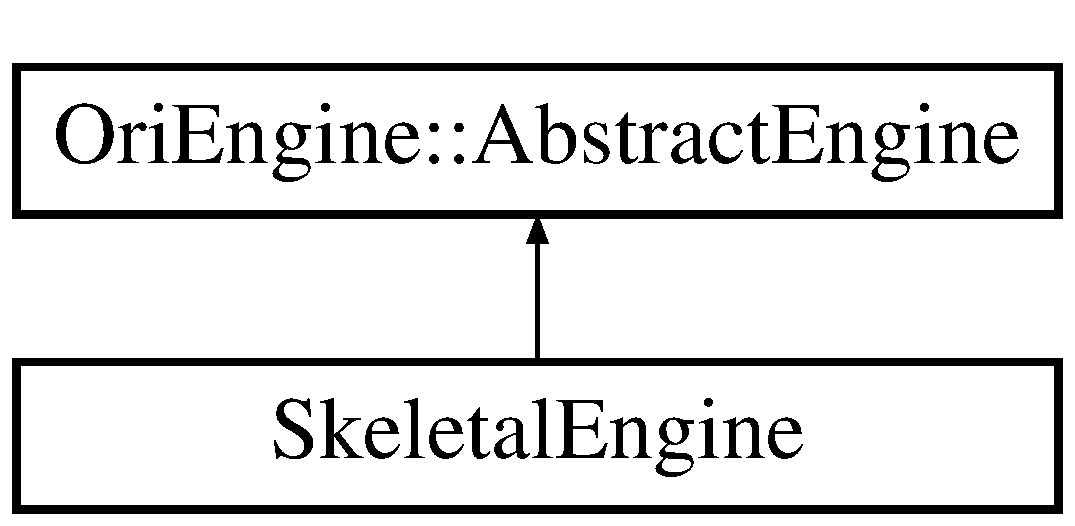
\includegraphics[height=2.000000cm]{class_ori_engine_1_1_abstract_engine}
\end{center}
\end{figure}
\subsection*{Public Member Functions}
\begin{DoxyCompactItemize}
\item 
virtual void \hyperlink{class_ori_engine_1_1_abstract_engine_a7359c90344c928e283d177159780646e}{on\+Create} ()=0
\item 
void \hyperlink{class_ori_engine_1_1_abstract_engine_ad969514426afbd6818caea13a538c565}{init} ()
\item 
virtual void \hyperlink{class_ori_engine_1_1_abstract_engine_a132e10c2452afe2d555ac85ea1b48845}{pre\+Render} (double time)
\item 
virtual void \hyperlink{class_ori_engine_1_1_abstract_engine_a12ce6df5383341e36fd674a5e026bf3f}{post\+Render} ()
\item 
void \hyperlink{class_ori_engine_1_1_abstract_engine_a6a9cec01e078695703f9def8e3814dbf}{end\+Render} ()
\item 
void \hyperlink{class_ori_engine_1_1_abstract_engine_ae406e1718ed7da4d0ff074f91bd2d4b7}{start\+Render} ()
\item 
void \hyperlink{class_ori_engine_1_1_abstract_engine_aa88ad7f1c4168f03139f33d467b0a9d0}{render} () const
\item 
void \hyperlink{class_ori_engine_1_1_abstract_engine_a8c77cd4669df9193d5283cf48bee3b94}{clean\+Up} ()
\item 
\hyperlink{class_ori_engine_1_1_abstract_renderer}{Abstract\+Renderer} $\ast$ \hyperlink{class_ori_engine_1_1_abstract_engine_a06eb88e86a88b9dbd392b6a789a3d91e}{get\+Renderer} ()
\item 
bool \hyperlink{class_ori_engine_1_1_abstract_engine_af02f0fa50c8ef658e3ff892aa8d8a264}{still\+Rendering} ()
\item 
std\+::string \hyperlink{class_ori_engine_1_1_abstract_engine_a41b34e146f5b19e40dc3f1cb1343d4d6}{get\+Name} ()
\item 
\hyperlink{class_ori_engine_1_1_abstract_engine_acb8473107540b7ed52eadce12bc69a81}{$\sim$\+Abstract\+Engine} ()
\item 
\hyperlink{class_ori_engine_1_1_abstract_engine_aca590b0d9aa8d7f6b907b2ea575f52d8}{Abstract\+Engine} ()
\end{DoxyCompactItemize}
\subsection*{Static Public Member Functions}
\begin{DoxyCompactItemize}
\item 
static \hyperlink{class_ori_engine_1_1_abstract_engine}{Abstract\+Engine} $\ast$ \hyperlink{class_ori_engine_1_1_abstract_engine_a650375136fb726707d36acbf9f7ed3b8}{get\+Instance} ()
\item 
static void \hyperlink{class_ori_engine_1_1_abstract_engine_a03fcd9fd70108afd53924b0f9d2724a3}{log} (\hyperlink{class_ori_engine_1_1_debug_logger_a3ac0c97517b3aecb4ea7bdb5b98e6fe5}{Debug\+Logger\+::\+Msg\+Type} msg\+Type, std\+::string method, std\+::string \+\_\+class, std\+::string file, int line, std\+::string msg)
\end{DoxyCompactItemize}
\subsection*{Public Attributes}
\begin{DoxyCompactItemize}
\item 
\hyperlink{class_ori_engine_1_1_open_gl_renderer}{Open\+Gl\+Renderer} $\ast$ \hyperlink{class_ori_engine_1_1_abstract_engine_ab1a0fbe17c1ddf528a9863b8b3e19d41}{renderer}
\end{DoxyCompactItemize}
\subsection*{Private Attributes}
\begin{DoxyCompactItemize}
\item 
std\+::string \hyperlink{class_ori_engine_1_1_abstract_engine_a0d5405beaacf6c596046a66986e7573a}{Application\+Name} = \char`\"{}Ori \hyperlink{_skeletal_engine_8cpp_a67e670c1f33b20215b3721b4a515deb2}{Engine}\char`\"{}
\item 
double \hyperlink{class_ori_engine_1_1_abstract_engine_a34aa336df066d8c50363cf6260fcd268}{game\+Start\+Time}
\item 
double \hyperlink{class_ori_engine_1_1_abstract_engine_a8b839c3500a3156be543f1119f280a81}{last\+Frame\+Finish\+Time}
\item 
double \hyperlink{class_ori_engine_1_1_abstract_engine_a28d43c329a702901905e6b2aee2f23f7}{last\+Frame\+Start\+Time}
\item 
double \hyperlink{class_ori_engine_1_1_abstract_engine_a98601d59527aa41d264c07ec6cfb3fde}{frame\+Avg\+Total}
\item 
int \hyperlink{class_ori_engine_1_1_abstract_engine_a878214e5c90997da1b783cd14eb19c6e}{frame\+Avg\+Number}
\item 
int \hyperlink{class_ori_engine_1_1_abstract_engine_ad6ff48352c89ad50432a017a167dd860}{frame\+Avg\+Max\+Number}
\item 
\hyperlink{class_ori_engine_1_1_window}{Window} $\ast$ \hyperlink{class_ori_engine_1_1_abstract_engine_a19fb6e3400090763c2459f7ee412ca14}{window}
\end{DoxyCompactItemize}
\subsection*{Static Private Attributes}
\begin{DoxyCompactItemize}
\item 
static \hyperlink{class_ori_engine_1_1_abstract_engine}{Abstract\+Engine} $\ast$ \hyperlink{class_ori_engine_1_1_abstract_engine_a2a20dacf864ea1a8136e7531fa901932}{app\+Instance} = nullptr
\end{DoxyCompactItemize}


\subsection{Constructor \& Destructor Documentation}
\hypertarget{class_ori_engine_1_1_abstract_engine_acb8473107540b7ed52eadce12bc69a81}{}\label{class_ori_engine_1_1_abstract_engine_acb8473107540b7ed52eadce12bc69a81} 
\index{Ori\+Engine\+::\+Abstract\+Engine@{Ori\+Engine\+::\+Abstract\+Engine}!````~Abstract\+Engine@{$\sim$\+Abstract\+Engine}}
\index{````~Abstract\+Engine@{$\sim$\+Abstract\+Engine}!Ori\+Engine\+::\+Abstract\+Engine@{Ori\+Engine\+::\+Abstract\+Engine}}
\subsubsection{\texorpdfstring{$\sim$\+Abstract\+Engine()}{~AbstractEngine()}}
{\footnotesize\ttfamily Abstract\+Engine\+::$\sim$\+Abstract\+Engine (\begin{DoxyParamCaption}{ }\end{DoxyParamCaption})}

\hypertarget{class_ori_engine_1_1_abstract_engine_aca590b0d9aa8d7f6b907b2ea575f52d8}{}\label{class_ori_engine_1_1_abstract_engine_aca590b0d9aa8d7f6b907b2ea575f52d8} 
\index{Ori\+Engine\+::\+Abstract\+Engine@{Ori\+Engine\+::\+Abstract\+Engine}!Abstract\+Engine@{Abstract\+Engine}}
\index{Abstract\+Engine@{Abstract\+Engine}!Ori\+Engine\+::\+Abstract\+Engine@{Ori\+Engine\+::\+Abstract\+Engine}}
\subsubsection{\texorpdfstring{Abstract\+Engine()}{AbstractEngine()}}
{\footnotesize\ttfamily Abstract\+Engine\+::\+Abstract\+Engine (\begin{DoxyParamCaption}{ }\end{DoxyParamCaption})}



\subsection{Member Function Documentation}
\hypertarget{class_ori_engine_1_1_abstract_engine_a8c77cd4669df9193d5283cf48bee3b94}{}\label{class_ori_engine_1_1_abstract_engine_a8c77cd4669df9193d5283cf48bee3b94} 
\index{Ori\+Engine\+::\+Abstract\+Engine@{Ori\+Engine\+::\+Abstract\+Engine}!clean\+Up@{clean\+Up}}
\index{clean\+Up@{clean\+Up}!Ori\+Engine\+::\+Abstract\+Engine@{Ori\+Engine\+::\+Abstract\+Engine}}
\subsubsection{\texorpdfstring{clean\+Up()}{cleanUp()}}
{\footnotesize\ttfamily void Abstract\+Engine\+::clean\+Up (\begin{DoxyParamCaption}{ }\end{DoxyParamCaption})}

\hypertarget{class_ori_engine_1_1_abstract_engine_a6a9cec01e078695703f9def8e3814dbf}{}\label{class_ori_engine_1_1_abstract_engine_a6a9cec01e078695703f9def8e3814dbf} 
\index{Ori\+Engine\+::\+Abstract\+Engine@{Ori\+Engine\+::\+Abstract\+Engine}!end\+Render@{end\+Render}}
\index{end\+Render@{end\+Render}!Ori\+Engine\+::\+Abstract\+Engine@{Ori\+Engine\+::\+Abstract\+Engine}}
\subsubsection{\texorpdfstring{end\+Render()}{endRender()}}
{\footnotesize\ttfamily void Abstract\+Engine\+::end\+Render (\begin{DoxyParamCaption}{ }\end{DoxyParamCaption})}

\hypertarget{class_ori_engine_1_1_abstract_engine_a650375136fb726707d36acbf9f7ed3b8}{}\label{class_ori_engine_1_1_abstract_engine_a650375136fb726707d36acbf9f7ed3b8} 
\index{Ori\+Engine\+::\+Abstract\+Engine@{Ori\+Engine\+::\+Abstract\+Engine}!get\+Instance@{get\+Instance}}
\index{get\+Instance@{get\+Instance}!Ori\+Engine\+::\+Abstract\+Engine@{Ori\+Engine\+::\+Abstract\+Engine}}
\subsubsection{\texorpdfstring{get\+Instance()}{getInstance()}}
{\footnotesize\ttfamily \hyperlink{class_ori_engine_1_1_abstract_engine}{Abstract\+Engine} $\ast$ Abstract\+Engine\+::get\+Instance (\begin{DoxyParamCaption}{ }\end{DoxyParamCaption})\hspace{0.3cm}{\ttfamily [static]}}

\hypertarget{class_ori_engine_1_1_abstract_engine_a41b34e146f5b19e40dc3f1cb1343d4d6}{}\label{class_ori_engine_1_1_abstract_engine_a41b34e146f5b19e40dc3f1cb1343d4d6} 
\index{Ori\+Engine\+::\+Abstract\+Engine@{Ori\+Engine\+::\+Abstract\+Engine}!get\+Name@{get\+Name}}
\index{get\+Name@{get\+Name}!Ori\+Engine\+::\+Abstract\+Engine@{Ori\+Engine\+::\+Abstract\+Engine}}
\subsubsection{\texorpdfstring{get\+Name()}{getName()}}
{\footnotesize\ttfamily std\+::string Ori\+Engine\+::\+Abstract\+Engine\+::get\+Name (\begin{DoxyParamCaption}{ }\end{DoxyParamCaption})\hspace{0.3cm}{\ttfamily [inline]}}

\hypertarget{class_ori_engine_1_1_abstract_engine_a06eb88e86a88b9dbd392b6a789a3d91e}{}\label{class_ori_engine_1_1_abstract_engine_a06eb88e86a88b9dbd392b6a789a3d91e} 
\index{Ori\+Engine\+::\+Abstract\+Engine@{Ori\+Engine\+::\+Abstract\+Engine}!get\+Renderer@{get\+Renderer}}
\index{get\+Renderer@{get\+Renderer}!Ori\+Engine\+::\+Abstract\+Engine@{Ori\+Engine\+::\+Abstract\+Engine}}
\subsubsection{\texorpdfstring{get\+Renderer()}{getRenderer()}}
{\footnotesize\ttfamily \hyperlink{class_ori_engine_1_1_abstract_renderer}{Abstract\+Renderer}$\ast$ Ori\+Engine\+::\+Abstract\+Engine\+::get\+Renderer (\begin{DoxyParamCaption}{ }\end{DoxyParamCaption})\hspace{0.3cm}{\ttfamily [inline]}}

\hypertarget{class_ori_engine_1_1_abstract_engine_ad969514426afbd6818caea13a538c565}{}\label{class_ori_engine_1_1_abstract_engine_ad969514426afbd6818caea13a538c565} 
\index{Ori\+Engine\+::\+Abstract\+Engine@{Ori\+Engine\+::\+Abstract\+Engine}!init@{init}}
\index{init@{init}!Ori\+Engine\+::\+Abstract\+Engine@{Ori\+Engine\+::\+Abstract\+Engine}}
\subsubsection{\texorpdfstring{init()}{init()}}
{\footnotesize\ttfamily void Abstract\+Engine\+::init (\begin{DoxyParamCaption}{ }\end{DoxyParamCaption})}

\hypertarget{class_ori_engine_1_1_abstract_engine_a03fcd9fd70108afd53924b0f9d2724a3}{}\label{class_ori_engine_1_1_abstract_engine_a03fcd9fd70108afd53924b0f9d2724a3} 
\index{Ori\+Engine\+::\+Abstract\+Engine@{Ori\+Engine\+::\+Abstract\+Engine}!log@{log}}
\index{log@{log}!Ori\+Engine\+::\+Abstract\+Engine@{Ori\+Engine\+::\+Abstract\+Engine}}
\subsubsection{\texorpdfstring{log()}{log()}}
{\footnotesize\ttfamily static void Ori\+Engine\+::\+Abstract\+Engine\+::log (\begin{DoxyParamCaption}\item[{\hyperlink{class_ori_engine_1_1_debug_logger_a3ac0c97517b3aecb4ea7bdb5b98e6fe5}{Debug\+Logger\+::\+Msg\+Type}}]{msg\+Type,  }\item[{std\+::string}]{method,  }\item[{std\+::string}]{\+\_\+class,  }\item[{std\+::string}]{file,  }\item[{int}]{line,  }\item[{std\+::string}]{msg }\end{DoxyParamCaption})\hspace{0.3cm}{\ttfamily [inline]}, {\ttfamily [static]}}

\hypertarget{class_ori_engine_1_1_abstract_engine_a7359c90344c928e283d177159780646e}{}\label{class_ori_engine_1_1_abstract_engine_a7359c90344c928e283d177159780646e} 
\index{Ori\+Engine\+::\+Abstract\+Engine@{Ori\+Engine\+::\+Abstract\+Engine}!on\+Create@{on\+Create}}
\index{on\+Create@{on\+Create}!Ori\+Engine\+::\+Abstract\+Engine@{Ori\+Engine\+::\+Abstract\+Engine}}
\subsubsection{\texorpdfstring{on\+Create()}{onCreate()}}
{\footnotesize\ttfamily void Abstract\+Engine\+::on\+Create (\begin{DoxyParamCaption}{ }\end{DoxyParamCaption})\hspace{0.3cm}{\ttfamily [pure virtual]}}



Implemented in \hyperlink{class_skeletal_engine_aa947bae905c4e4628bfe5036b4943a08}{Skeletal\+Engine}.

\hypertarget{class_ori_engine_1_1_abstract_engine_a12ce6df5383341e36fd674a5e026bf3f}{}\label{class_ori_engine_1_1_abstract_engine_a12ce6df5383341e36fd674a5e026bf3f} 
\index{Ori\+Engine\+::\+Abstract\+Engine@{Ori\+Engine\+::\+Abstract\+Engine}!post\+Render@{post\+Render}}
\index{post\+Render@{post\+Render}!Ori\+Engine\+::\+Abstract\+Engine@{Ori\+Engine\+::\+Abstract\+Engine}}
\subsubsection{\texorpdfstring{post\+Render()}{postRender()}}
{\footnotesize\ttfamily void Abstract\+Engine\+::post\+Render (\begin{DoxyParamCaption}{ }\end{DoxyParamCaption})\hspace{0.3cm}{\ttfamily [virtual]}}



Reimplemented in \hyperlink{class_skeletal_engine_a58981a23dad5e0bf14aadede98bba12f}{Skeletal\+Engine}.

\hypertarget{class_ori_engine_1_1_abstract_engine_a132e10c2452afe2d555ac85ea1b48845}{}\label{class_ori_engine_1_1_abstract_engine_a132e10c2452afe2d555ac85ea1b48845} 
\index{Ori\+Engine\+::\+Abstract\+Engine@{Ori\+Engine\+::\+Abstract\+Engine}!pre\+Render@{pre\+Render}}
\index{pre\+Render@{pre\+Render}!Ori\+Engine\+::\+Abstract\+Engine@{Ori\+Engine\+::\+Abstract\+Engine}}
\subsubsection{\texorpdfstring{pre\+Render()}{preRender()}}
{\footnotesize\ttfamily void Abstract\+Engine\+::pre\+Render (\begin{DoxyParamCaption}\item[{double}]{time }\end{DoxyParamCaption})\hspace{0.3cm}{\ttfamily [virtual]}}



Reimplemented in \hyperlink{class_skeletal_engine_a9d3352322b1c4c8aa6332765e8efcde6}{Skeletal\+Engine}.

\hypertarget{class_ori_engine_1_1_abstract_engine_aa88ad7f1c4168f03139f33d467b0a9d0}{}\label{class_ori_engine_1_1_abstract_engine_aa88ad7f1c4168f03139f33d467b0a9d0} 
\index{Ori\+Engine\+::\+Abstract\+Engine@{Ori\+Engine\+::\+Abstract\+Engine}!render@{render}}
\index{render@{render}!Ori\+Engine\+::\+Abstract\+Engine@{Ori\+Engine\+::\+Abstract\+Engine}}
\subsubsection{\texorpdfstring{render()}{render()}}
{\footnotesize\ttfamily void Abstract\+Engine\+::render (\begin{DoxyParamCaption}{ }\end{DoxyParamCaption}) const}

\hypertarget{class_ori_engine_1_1_abstract_engine_ae406e1718ed7da4d0ff074f91bd2d4b7}{}\label{class_ori_engine_1_1_abstract_engine_ae406e1718ed7da4d0ff074f91bd2d4b7} 
\index{Ori\+Engine\+::\+Abstract\+Engine@{Ori\+Engine\+::\+Abstract\+Engine}!start\+Render@{start\+Render}}
\index{start\+Render@{start\+Render}!Ori\+Engine\+::\+Abstract\+Engine@{Ori\+Engine\+::\+Abstract\+Engine}}
\subsubsection{\texorpdfstring{start\+Render()}{startRender()}}
{\footnotesize\ttfamily void Abstract\+Engine\+::start\+Render (\begin{DoxyParamCaption}{ }\end{DoxyParamCaption})}

\hypertarget{class_ori_engine_1_1_abstract_engine_af02f0fa50c8ef658e3ff892aa8d8a264}{}\label{class_ori_engine_1_1_abstract_engine_af02f0fa50c8ef658e3ff892aa8d8a264} 
\index{Ori\+Engine\+::\+Abstract\+Engine@{Ori\+Engine\+::\+Abstract\+Engine}!still\+Rendering@{still\+Rendering}}
\index{still\+Rendering@{still\+Rendering}!Ori\+Engine\+::\+Abstract\+Engine@{Ori\+Engine\+::\+Abstract\+Engine}}
\subsubsection{\texorpdfstring{still\+Rendering()}{stillRendering()}}
{\footnotesize\ttfamily bool Ori\+Engine\+::\+Abstract\+Engine\+::still\+Rendering (\begin{DoxyParamCaption}{ }\end{DoxyParamCaption})\hspace{0.3cm}{\ttfamily [inline]}}



\subsection{Member Data Documentation}
\hypertarget{class_ori_engine_1_1_abstract_engine_a2a20dacf864ea1a8136e7531fa901932}{}\label{class_ori_engine_1_1_abstract_engine_a2a20dacf864ea1a8136e7531fa901932} 
\index{Ori\+Engine\+::\+Abstract\+Engine@{Ori\+Engine\+::\+Abstract\+Engine}!app\+Instance@{app\+Instance}}
\index{app\+Instance@{app\+Instance}!Ori\+Engine\+::\+Abstract\+Engine@{Ori\+Engine\+::\+Abstract\+Engine}}
\subsubsection{\texorpdfstring{app\+Instance}{appInstance}}
{\footnotesize\ttfamily \hyperlink{class_ori_engine_1_1_abstract_engine}{Abstract\+Engine} $\ast$ Abstract\+Engine\+::app\+Instance = nullptr\hspace{0.3cm}{\ttfamily [static]}, {\ttfamily [private]}}

\hypertarget{class_ori_engine_1_1_abstract_engine_a0d5405beaacf6c596046a66986e7573a}{}\label{class_ori_engine_1_1_abstract_engine_a0d5405beaacf6c596046a66986e7573a} 
\index{Ori\+Engine\+::\+Abstract\+Engine@{Ori\+Engine\+::\+Abstract\+Engine}!Application\+Name@{Application\+Name}}
\index{Application\+Name@{Application\+Name}!Ori\+Engine\+::\+Abstract\+Engine@{Ori\+Engine\+::\+Abstract\+Engine}}
\subsubsection{\texorpdfstring{Application\+Name}{ApplicationName}}
{\footnotesize\ttfamily std\+::string Ori\+Engine\+::\+Abstract\+Engine\+::\+Application\+Name = \char`\"{}Ori \hyperlink{_skeletal_engine_8cpp_a67e670c1f33b20215b3721b4a515deb2}{Engine}\char`\"{}\hspace{0.3cm}{\ttfamily [private]}}

\hypertarget{class_ori_engine_1_1_abstract_engine_ad6ff48352c89ad50432a017a167dd860}{}\label{class_ori_engine_1_1_abstract_engine_ad6ff48352c89ad50432a017a167dd860} 
\index{Ori\+Engine\+::\+Abstract\+Engine@{Ori\+Engine\+::\+Abstract\+Engine}!frame\+Avg\+Max\+Number@{frame\+Avg\+Max\+Number}}
\index{frame\+Avg\+Max\+Number@{frame\+Avg\+Max\+Number}!Ori\+Engine\+::\+Abstract\+Engine@{Ori\+Engine\+::\+Abstract\+Engine}}
\subsubsection{\texorpdfstring{frame\+Avg\+Max\+Number}{frameAvgMaxNumber}}
{\footnotesize\ttfamily int Ori\+Engine\+::\+Abstract\+Engine\+::frame\+Avg\+Max\+Number\hspace{0.3cm}{\ttfamily [private]}}

The maximum number of frames used to calculate the frame rate \hypertarget{class_ori_engine_1_1_abstract_engine_a878214e5c90997da1b783cd14eb19c6e}{}\label{class_ori_engine_1_1_abstract_engine_a878214e5c90997da1b783cd14eb19c6e} 
\index{Ori\+Engine\+::\+Abstract\+Engine@{Ori\+Engine\+::\+Abstract\+Engine}!frame\+Avg\+Number@{frame\+Avg\+Number}}
\index{frame\+Avg\+Number@{frame\+Avg\+Number}!Ori\+Engine\+::\+Abstract\+Engine@{Ori\+Engine\+::\+Abstract\+Engine}}
\subsubsection{\texorpdfstring{frame\+Avg\+Number}{frameAvgNumber}}
{\footnotesize\ttfamily int Ori\+Engine\+::\+Abstract\+Engine\+::frame\+Avg\+Number\hspace{0.3cm}{\ttfamily [private]}}

A count of the number of frames in the current total \hypertarget{class_ori_engine_1_1_abstract_engine_a98601d59527aa41d264c07ec6cfb3fde}{}\label{class_ori_engine_1_1_abstract_engine_a98601d59527aa41d264c07ec6cfb3fde} 
\index{Ori\+Engine\+::\+Abstract\+Engine@{Ori\+Engine\+::\+Abstract\+Engine}!frame\+Avg\+Total@{frame\+Avg\+Total}}
\index{frame\+Avg\+Total@{frame\+Avg\+Total}!Ori\+Engine\+::\+Abstract\+Engine@{Ori\+Engine\+::\+Abstract\+Engine}}
\subsubsection{\texorpdfstring{frame\+Avg\+Total}{frameAvgTotal}}
{\footnotesize\ttfamily double Ori\+Engine\+::\+Abstract\+Engine\+::frame\+Avg\+Total\hspace{0.3cm}{\ttfamily [private]}}

An accumulator used to add time for last few avg frames to calc frame rate \hypertarget{class_ori_engine_1_1_abstract_engine_a34aa336df066d8c50363cf6260fcd268}{}\label{class_ori_engine_1_1_abstract_engine_a34aa336df066d8c50363cf6260fcd268} 
\index{Ori\+Engine\+::\+Abstract\+Engine@{Ori\+Engine\+::\+Abstract\+Engine}!game\+Start\+Time@{game\+Start\+Time}}
\index{game\+Start\+Time@{game\+Start\+Time}!Ori\+Engine\+::\+Abstract\+Engine@{Ori\+Engine\+::\+Abstract\+Engine}}
\subsubsection{\texorpdfstring{game\+Start\+Time}{gameStartTime}}
{\footnotesize\ttfamily double Ori\+Engine\+::\+Abstract\+Engine\+::game\+Start\+Time\hspace{0.3cm}{\ttfamily [private]}}

\hypertarget{class_ori_engine_1_1_abstract_engine_a8b839c3500a3156be543f1119f280a81}{}\label{class_ori_engine_1_1_abstract_engine_a8b839c3500a3156be543f1119f280a81} 
\index{Ori\+Engine\+::\+Abstract\+Engine@{Ori\+Engine\+::\+Abstract\+Engine}!last\+Frame\+Finish\+Time@{last\+Frame\+Finish\+Time}}
\index{last\+Frame\+Finish\+Time@{last\+Frame\+Finish\+Time}!Ori\+Engine\+::\+Abstract\+Engine@{Ori\+Engine\+::\+Abstract\+Engine}}
\subsubsection{\texorpdfstring{last\+Frame\+Finish\+Time}{lastFrameFinishTime}}
{\footnotesize\ttfamily double Ori\+Engine\+::\+Abstract\+Engine\+::last\+Frame\+Finish\+Time\hspace{0.3cm}{\ttfamily [private]}}

The time the last frame rendering was complete \hypertarget{class_ori_engine_1_1_abstract_engine_a28d43c329a702901905e6b2aee2f23f7}{}\label{class_ori_engine_1_1_abstract_engine_a28d43c329a702901905e6b2aee2f23f7} 
\index{Ori\+Engine\+::\+Abstract\+Engine@{Ori\+Engine\+::\+Abstract\+Engine}!last\+Frame\+Start\+Time@{last\+Frame\+Start\+Time}}
\index{last\+Frame\+Start\+Time@{last\+Frame\+Start\+Time}!Ori\+Engine\+::\+Abstract\+Engine@{Ori\+Engine\+::\+Abstract\+Engine}}
\subsubsection{\texorpdfstring{last\+Frame\+Start\+Time}{lastFrameStartTime}}
{\footnotesize\ttfamily double Ori\+Engine\+::\+Abstract\+Engine\+::last\+Frame\+Start\+Time\hspace{0.3cm}{\ttfamily [private]}}

The time the last frame started rendering \hypertarget{class_ori_engine_1_1_abstract_engine_ab1a0fbe17c1ddf528a9863b8b3e19d41}{}\label{class_ori_engine_1_1_abstract_engine_ab1a0fbe17c1ddf528a9863b8b3e19d41} 
\index{Ori\+Engine\+::\+Abstract\+Engine@{Ori\+Engine\+::\+Abstract\+Engine}!renderer@{renderer}}
\index{renderer@{renderer}!Ori\+Engine\+::\+Abstract\+Engine@{Ori\+Engine\+::\+Abstract\+Engine}}
\subsubsection{\texorpdfstring{renderer}{renderer}}
{\footnotesize\ttfamily \hyperlink{class_ori_engine_1_1_open_gl_renderer}{Open\+Gl\+Renderer}$\ast$ Ori\+Engine\+::\+Abstract\+Engine\+::renderer}

\hypertarget{class_ori_engine_1_1_abstract_engine_a19fb6e3400090763c2459f7ee412ca14}{}\label{class_ori_engine_1_1_abstract_engine_a19fb6e3400090763c2459f7ee412ca14} 
\index{Ori\+Engine\+::\+Abstract\+Engine@{Ori\+Engine\+::\+Abstract\+Engine}!window@{window}}
\index{window@{window}!Ori\+Engine\+::\+Abstract\+Engine@{Ori\+Engine\+::\+Abstract\+Engine}}
\subsubsection{\texorpdfstring{window}{window}}
{\footnotesize\ttfamily \hyperlink{class_ori_engine_1_1_window}{Window}$\ast$ Ori\+Engine\+::\+Abstract\+Engine\+::window\hspace{0.3cm}{\ttfamily [private]}}



The documentation for this class was generated from the following files\+:\begin{DoxyCompactItemize}
\item 
Ori\+Engine/\+Ori\+Engine/\hyperlink{_abstract_engine_8h}{Abstract\+Engine.\+h}\item 
Ori\+Engine/\+Ori\+Engine/\hyperlink{_abstract_engine_8cpp}{Abstract\+Engine.\+cpp}\end{DoxyCompactItemize}

\hypertarget{class_ori_engine_1_1_abstract_renderer}{}\section{Ori\+Engine\+:\+:Abstract\+Renderer Class Reference}
\label{class_ori_engine_1_1_abstract_renderer}\index{Ori\+Engine\+::\+Abstract\+Renderer@{Ori\+Engine\+::\+Abstract\+Renderer}}


{\ttfamily \#include $<$Abstract\+Renderer.\+h$>$}

Inheritance diagram for Ori\+Engine\+:\+:Abstract\+Renderer\+:\begin{figure}[H]
\begin{center}
\leavevmode
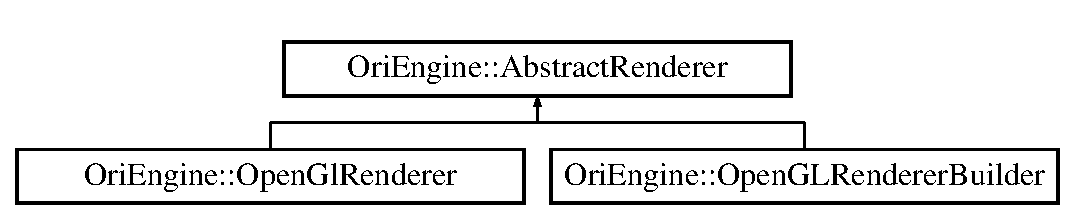
\includegraphics[height=2.000000cm]{class_ori_engine_1_1_abstract_renderer}
\end{center}
\end{figure}
\subsection*{Public Member Functions}
\begin{DoxyCompactItemize}
\item 
\hyperlink{class_ori_engine_1_1_abstract_renderer_ad9010e136537af7bce43e5334868f69b}{Abstract\+Renderer} ()
\item 
virtual \hyperlink{class_ori_engine_1_1_abstract_renderer_a7bdef22326c436a4152632180d98bc6e}{$\sim$\+Abstract\+Renderer} ()
\item 
virtual void \hyperlink{class_ori_engine_1_1_abstract_renderer_aece5371f0d8b99e6ee456845aba89f8d}{draw\+Primative} ()=0
\item 
virtual void \hyperlink{class_ori_engine_1_1_abstract_renderer_a2af2aba80028b0aa4cca39097e1fdf6d}{init} ()=0
\item 
virtual void \hyperlink{class_ori_engine_1_1_abstract_renderer_a978fc31cfc5fc8c2cafa3d33367fdb32}{version\+Info} ()=0
\end{DoxyCompactItemize}


\subsection{Constructor \& Destructor Documentation}
\hypertarget{class_ori_engine_1_1_abstract_renderer_ad9010e136537af7bce43e5334868f69b}{}\label{class_ori_engine_1_1_abstract_renderer_ad9010e136537af7bce43e5334868f69b} 
\index{Ori\+Engine\+::\+Abstract\+Renderer@{Ori\+Engine\+::\+Abstract\+Renderer}!Abstract\+Renderer@{Abstract\+Renderer}}
\index{Abstract\+Renderer@{Abstract\+Renderer}!Ori\+Engine\+::\+Abstract\+Renderer@{Ori\+Engine\+::\+Abstract\+Renderer}}
\subsubsection{\texorpdfstring{Abstract\+Renderer()}{AbstractRenderer()}}
{\footnotesize\ttfamily Ori\+Engine\+::\+Abstract\+Renderer\+::\+Abstract\+Renderer (\begin{DoxyParamCaption}{ }\end{DoxyParamCaption})\hspace{0.3cm}{\ttfamily [inline]}}

\hypertarget{class_ori_engine_1_1_abstract_renderer_a7bdef22326c436a4152632180d98bc6e}{}\label{class_ori_engine_1_1_abstract_renderer_a7bdef22326c436a4152632180d98bc6e} 
\index{Ori\+Engine\+::\+Abstract\+Renderer@{Ori\+Engine\+::\+Abstract\+Renderer}!````~Abstract\+Renderer@{$\sim$\+Abstract\+Renderer}}
\index{````~Abstract\+Renderer@{$\sim$\+Abstract\+Renderer}!Ori\+Engine\+::\+Abstract\+Renderer@{Ori\+Engine\+::\+Abstract\+Renderer}}
\subsubsection{\texorpdfstring{$\sim$\+Abstract\+Renderer()}{~AbstractRenderer()}}
{\footnotesize\ttfamily Abstract\+Renderer\+::$\sim$\+Abstract\+Renderer (\begin{DoxyParamCaption}{ }\end{DoxyParamCaption})\hspace{0.3cm}{\ttfamily [virtual]}}



\subsection{Member Function Documentation}
\hypertarget{class_ori_engine_1_1_abstract_renderer_aece5371f0d8b99e6ee456845aba89f8d}{}\label{class_ori_engine_1_1_abstract_renderer_aece5371f0d8b99e6ee456845aba89f8d} 
\index{Ori\+Engine\+::\+Abstract\+Renderer@{Ori\+Engine\+::\+Abstract\+Renderer}!draw\+Primative@{draw\+Primative}}
\index{draw\+Primative@{draw\+Primative}!Ori\+Engine\+::\+Abstract\+Renderer@{Ori\+Engine\+::\+Abstract\+Renderer}}
\subsubsection{\texorpdfstring{draw\+Primative()}{drawPrimative()}}
{\footnotesize\ttfamily virtual void Ori\+Engine\+::\+Abstract\+Renderer\+::draw\+Primative (\begin{DoxyParamCaption}{ }\end{DoxyParamCaption})\hspace{0.3cm}{\ttfamily [pure virtual]}}



Implemented in \hyperlink{class_ori_engine_1_1_open_gl_renderer_ad75e25784e6aa3331f69b81b1b3774ff}{Ori\+Engine\+::\+Open\+Gl\+Renderer}.

\hypertarget{class_ori_engine_1_1_abstract_renderer_a2af2aba80028b0aa4cca39097e1fdf6d}{}\label{class_ori_engine_1_1_abstract_renderer_a2af2aba80028b0aa4cca39097e1fdf6d} 
\index{Ori\+Engine\+::\+Abstract\+Renderer@{Ori\+Engine\+::\+Abstract\+Renderer}!init@{init}}
\index{init@{init}!Ori\+Engine\+::\+Abstract\+Renderer@{Ori\+Engine\+::\+Abstract\+Renderer}}
\subsubsection{\texorpdfstring{init()}{init()}}
{\footnotesize\ttfamily virtual void Ori\+Engine\+::\+Abstract\+Renderer\+::init (\begin{DoxyParamCaption}{ }\end{DoxyParamCaption})\hspace{0.3cm}{\ttfamily [pure virtual]}}



Implemented in \hyperlink{class_ori_engine_1_1_open_gl_renderer_a702c4cfb099f77a04111740b9f3834e8}{Ori\+Engine\+::\+Open\+Gl\+Renderer}.

\hypertarget{class_ori_engine_1_1_abstract_renderer_a978fc31cfc5fc8c2cafa3d33367fdb32}{}\label{class_ori_engine_1_1_abstract_renderer_a978fc31cfc5fc8c2cafa3d33367fdb32} 
\index{Ori\+Engine\+::\+Abstract\+Renderer@{Ori\+Engine\+::\+Abstract\+Renderer}!version\+Info@{version\+Info}}
\index{version\+Info@{version\+Info}!Ori\+Engine\+::\+Abstract\+Renderer@{Ori\+Engine\+::\+Abstract\+Renderer}}
\subsubsection{\texorpdfstring{version\+Info()}{versionInfo()}}
{\footnotesize\ttfamily virtual void Ori\+Engine\+::\+Abstract\+Renderer\+::version\+Info (\begin{DoxyParamCaption}{ }\end{DoxyParamCaption})\hspace{0.3cm}{\ttfamily [pure virtual]}}



Implemented in \hyperlink{class_ori_engine_1_1_open_gl_renderer_aaf6633305987ddf18d0a6e5e15e93352}{Ori\+Engine\+::\+Open\+Gl\+Renderer}.



The documentation for this class was generated from the following files\+:\begin{DoxyCompactItemize}
\item 
Ori\+Engine/\+Ori\+Engine/\hyperlink{_abstract_renderer_8h}{Abstract\+Renderer.\+h}\item 
Ori\+Engine/\+Ori\+Engine/\hyperlink{_abstract_renderer_8cpp}{Abstract\+Renderer.\+cpp}\end{DoxyCompactItemize}

\hypertarget{class_ori_engine_1_1_abstract_renderer_builder}{}\section{Ori\+Engine\+:\+:Abstract\+Renderer\+Builder Class Reference}
\label{class_ori_engine_1_1_abstract_renderer_builder}\index{Ori\+Engine\+::\+Abstract\+Renderer\+Builder@{Ori\+Engine\+::\+Abstract\+Renderer\+Builder}}


{\ttfamily \#include $<$Abstract\+Renderer.\+h$>$}

\subsection*{Public Member Functions}
\begin{DoxyCompactItemize}
\item 
virtual \hyperlink{class_ori_engine_1_1_abstract_renderer}{Abstract\+Renderer} $\ast$ \hyperlink{class_ori_engine_1_1_abstract_renderer_builder_a15d2618b23fdbfa81fe80c02135871ca}{create\+Renderer} ()=0
\end{DoxyCompactItemize}


\subsection{Member Function Documentation}
\hypertarget{class_ori_engine_1_1_abstract_renderer_builder_a15d2618b23fdbfa81fe80c02135871ca}{}\label{class_ori_engine_1_1_abstract_renderer_builder_a15d2618b23fdbfa81fe80c02135871ca} 
\index{Ori\+Engine\+::\+Abstract\+Renderer\+Builder@{Ori\+Engine\+::\+Abstract\+Renderer\+Builder}!create\+Renderer@{create\+Renderer}}
\index{create\+Renderer@{create\+Renderer}!Ori\+Engine\+::\+Abstract\+Renderer\+Builder@{Ori\+Engine\+::\+Abstract\+Renderer\+Builder}}
\subsubsection{\texorpdfstring{create\+Renderer()}{createRenderer()}}
{\footnotesize\ttfamily virtual \hyperlink{class_ori_engine_1_1_abstract_renderer}{Abstract\+Renderer}$\ast$ Ori\+Engine\+::\+Abstract\+Renderer\+Builder\+::create\+Renderer (\begin{DoxyParamCaption}{ }\end{DoxyParamCaption})\hspace{0.3cm}{\ttfamily [pure virtual]}}



The documentation for this class was generated from the following file\+:\begin{DoxyCompactItemize}
\item 
Ori\+Engine/\+Ori\+Engine/\hyperlink{_abstract_renderer_8h}{Abstract\+Renderer.\+h}\end{DoxyCompactItemize}

\hypertarget{class_base_manager}{}\section{Base\+Manager Class Reference}
\label{class_base_manager}\index{Base\+Manager@{Base\+Manager}}


{\ttfamily \#include $<$Base\+Manager.\+h$>$}

\subsection*{Public Member Functions}
\begin{DoxyCompactItemize}
\item 
\hyperlink{class_base_manager_a663ef30d41792bdecf2598a6285cfddd}{Base\+Manager} ()
\item 
\hyperlink{class_base_manager_af512e2d3b2a7727a2766a6c95a6b90a3}{$\sim$\+Base\+Manager} ()
\item 
\hyperlink{class_base_manager}{Base\+Manager} $\ast$ \hyperlink{class_base_manager_af85c9b7676acfa30dd14e5f7a878c3fa}{get\+Manager} ()
\end{DoxyCompactItemize}
\subsection*{Private Attributes}
\begin{DoxyCompactItemize}
\item 
\hyperlink{class_base_manager}{Base\+Manager} $\ast$ \hyperlink{class_base_manager_ae53c7fd979ff30128ef75bafe87a2ee8}{manager\+Instance}
\end{DoxyCompactItemize}


\subsection{Constructor \& Destructor Documentation}
\hypertarget{class_base_manager_a663ef30d41792bdecf2598a6285cfddd}{}\label{class_base_manager_a663ef30d41792bdecf2598a6285cfddd} 
\index{Base\+Manager@{Base\+Manager}!Base\+Manager@{Base\+Manager}}
\index{Base\+Manager@{Base\+Manager}!Base\+Manager@{Base\+Manager}}
\subsubsection{\texorpdfstring{Base\+Manager()}{BaseManager()}}
{\footnotesize\ttfamily Base\+Manager\+::\+Base\+Manager (\begin{DoxyParamCaption}{ }\end{DoxyParamCaption})}

\hypertarget{class_base_manager_af512e2d3b2a7727a2766a6c95a6b90a3}{}\label{class_base_manager_af512e2d3b2a7727a2766a6c95a6b90a3} 
\index{Base\+Manager@{Base\+Manager}!````~Base\+Manager@{$\sim$\+Base\+Manager}}
\index{````~Base\+Manager@{$\sim$\+Base\+Manager}!Base\+Manager@{Base\+Manager}}
\subsubsection{\texorpdfstring{$\sim$\+Base\+Manager()}{~BaseManager()}}
{\footnotesize\ttfamily Base\+Manager\+::$\sim$\+Base\+Manager (\begin{DoxyParamCaption}{ }\end{DoxyParamCaption})}



\subsection{Member Function Documentation}
\hypertarget{class_base_manager_af85c9b7676acfa30dd14e5f7a878c3fa}{}\label{class_base_manager_af85c9b7676acfa30dd14e5f7a878c3fa} 
\index{Base\+Manager@{Base\+Manager}!get\+Manager@{get\+Manager}}
\index{get\+Manager@{get\+Manager}!Base\+Manager@{Base\+Manager}}
\subsubsection{\texorpdfstring{get\+Manager()}{getManager()}}
{\footnotesize\ttfamily \hyperlink{class_base_manager}{Base\+Manager}$\ast$ Base\+Manager\+::get\+Manager (\begin{DoxyParamCaption}{ }\end{DoxyParamCaption})}



\subsection{Member Data Documentation}
\hypertarget{class_base_manager_ae53c7fd979ff30128ef75bafe87a2ee8}{}\label{class_base_manager_ae53c7fd979ff30128ef75bafe87a2ee8} 
\index{Base\+Manager@{Base\+Manager}!manager\+Instance@{manager\+Instance}}
\index{manager\+Instance@{manager\+Instance}!Base\+Manager@{Base\+Manager}}
\subsubsection{\texorpdfstring{manager\+Instance}{managerInstance}}
{\footnotesize\ttfamily \hyperlink{class_base_manager}{Base\+Manager}$\ast$ Base\+Manager\+::manager\+Instance\hspace{0.3cm}{\ttfamily [private]}}



The documentation for this class was generated from the following files\+:\begin{DoxyCompactItemize}
\item 
Ori\+Engine/\+Ori\+Engine/\hyperlink{_base_manager_8h}{Base\+Manager.\+h}\item 
Ori\+Engine/\+Ori\+Engine/\hyperlink{_base_manager_8cpp}{Base\+Manager.\+cpp}\end{DoxyCompactItemize}

\hypertarget{class_ori_engine_1_1_clock}{}\section{Ori\+Engine\+:\+:Clock Class Reference}
\label{class_ori_engine_1_1_clock}\index{Ori\+Engine\+::\+Clock@{Ori\+Engine\+::\+Clock}}


{\ttfamily \#include $<$Clock.\+h$>$}

\subsection*{Public Member Functions}
\begin{DoxyCompactItemize}
\item 
\hyperlink{class_ori_engine_1_1_clock_afc976ce68fa85e15cc06f9ed47bddb7c}{$\sim$\+Clock} ()
\end{DoxyCompactItemize}
\subsection*{Static Public Member Functions}
\begin{DoxyCompactItemize}
\item 
static L\+A\+R\+G\+E\+\_\+\+I\+N\+T\+E\+G\+ER \hyperlink{class_ori_engine_1_1_clock_aace1360f2c2588f877a349af1b6e292e}{get\+Counter\+Difference} (L\+A\+R\+G\+E\+\_\+\+I\+N\+T\+E\+G\+ER s, L\+A\+R\+G\+E\+\_\+\+I\+N\+T\+E\+G\+ER e)
\item 
static double \hyperlink{class_ori_engine_1_1_clock_ae7323d08dc94df712cc7ebb8436eba63}{last\+Frame} (double now, double last)
\item 
static L\+A\+R\+G\+E\+\_\+\+I\+N\+T\+E\+G\+ER \hyperlink{class_ori_engine_1_1_clock_aa084e2f95ad8ef19c2b346cd98b76cf1}{get\+Current\+Ticks} ()
\item 
static void \hyperlink{class_ori_engine_1_1_clock_aef03f6bf516fba7b5e79c9dd8b4d1f60}{get\+Frequency} (L\+A\+R\+G\+E\+\_\+\+I\+N\+T\+E\+G\+ER frequency)
\item 
static double \hyperlink{class_ori_engine_1_1_clock_addeddeb3e238c9f9d7c8f9b5e639fe18}{get\+Time} ()
\item 
static L\+A\+R\+G\+E\+\_\+\+I\+N\+T\+E\+G\+ER \hyperlink{class_ori_engine_1_1_clock_a1963f95715596314a277e77401e42e38}{get\+Ticks} ()
\item 
static void \hyperlink{class_ori_engine_1_1_clock_aa89ec268b0bb79f4caa36c4aa50980b8}{elapsed\+Time} ()
\item 
static void \hyperlink{class_ori_engine_1_1_clock_aadaf546dbfb57577d2a9b0e9e4c95123}{init} ()
\item 
static double \hyperlink{class_ori_engine_1_1_clock_af05b430c26528f81d4c0ea530bfc3710}{ticks\+To\+Seconds} (L\+A\+R\+G\+E\+\_\+\+I\+N\+T\+E\+G\+ER ticks)
\end{DoxyCompactItemize}
\subsection*{Static Public Attributes}
\begin{DoxyCompactItemize}
\item 
static L\+A\+R\+G\+E\+\_\+\+I\+N\+T\+E\+G\+ER \hyperlink{class_ori_engine_1_1_clock_abe3180bfe2b7ae463f5ee6ce0e21e7c1}{counter}
\item 
static L\+A\+R\+G\+E\+\_\+\+I\+N\+T\+E\+G\+ER \hyperlink{class_ori_engine_1_1_clock_a38fb078b0bae590ca4ef633654082385}{time}
\item 
static L\+A\+R\+G\+E\+\_\+\+I\+N\+T\+E\+G\+ER \hyperlink{class_ori_engine_1_1_clock_af7e7d35c38fb0c2caec5e60b4b54d967}{freq}
\item 
static double \hyperlink{class_ori_engine_1_1_clock_a787b0d8adf09d20da696f502658cbcfb}{start}
\item 
static double \hyperlink{class_ori_engine_1_1_clock_afc43c686502126feebf54a99783dc7fd}{end}
\item 
static double \hyperlink{class_ori_engine_1_1_clock_afd164eb5b041271fe67e2c85ffb4c455}{delta\+Time}
\item 
static bool \hyperlink{class_ori_engine_1_1_clock_a30554fc8e22a92ae8b26ef881b802828}{high\+Res\+Clock} = false
\end{DoxyCompactItemize}
\subsection*{Private Member Functions}
\begin{DoxyCompactItemize}
\item 
\hyperlink{class_ori_engine_1_1_clock_adbc370eb6b5f8d01645cf440188160a8}{Clock} ()
\end{DoxyCompactItemize}


\subsection{Constructor \& Destructor Documentation}
\hypertarget{class_ori_engine_1_1_clock_afc976ce68fa85e15cc06f9ed47bddb7c}{}\label{class_ori_engine_1_1_clock_afc976ce68fa85e15cc06f9ed47bddb7c} 
\index{Ori\+Engine\+::\+Clock@{Ori\+Engine\+::\+Clock}!````~Clock@{$\sim$\+Clock}}
\index{````~Clock@{$\sim$\+Clock}!Ori\+Engine\+::\+Clock@{Ori\+Engine\+::\+Clock}}
\subsubsection{\texorpdfstring{$\sim$\+Clock()}{~Clock()}}
{\footnotesize\ttfamily Clock\+::$\sim$\+Clock (\begin{DoxyParamCaption}{ }\end{DoxyParamCaption})}

\hypertarget{class_ori_engine_1_1_clock_adbc370eb6b5f8d01645cf440188160a8}{}\label{class_ori_engine_1_1_clock_adbc370eb6b5f8d01645cf440188160a8} 
\index{Ori\+Engine\+::\+Clock@{Ori\+Engine\+::\+Clock}!Clock@{Clock}}
\index{Clock@{Clock}!Ori\+Engine\+::\+Clock@{Ori\+Engine\+::\+Clock}}
\subsubsection{\texorpdfstring{Clock()}{Clock()}}
{\footnotesize\ttfamily Clock\+::\+Clock (\begin{DoxyParamCaption}{ }\end{DoxyParamCaption})\hspace{0.3cm}{\ttfamily [private]}}



\subsection{Member Function Documentation}
\hypertarget{class_ori_engine_1_1_clock_aa89ec268b0bb79f4caa36c4aa50980b8}{}\label{class_ori_engine_1_1_clock_aa89ec268b0bb79f4caa36c4aa50980b8} 
\index{Ori\+Engine\+::\+Clock@{Ori\+Engine\+::\+Clock}!elapsed\+Time@{elapsed\+Time}}
\index{elapsed\+Time@{elapsed\+Time}!Ori\+Engine\+::\+Clock@{Ori\+Engine\+::\+Clock}}
\subsubsection{\texorpdfstring{elapsed\+Time()}{elapsedTime()}}
{\footnotesize\ttfamily void Clock\+::elapsed\+Time (\begin{DoxyParamCaption}{ }\end{DoxyParamCaption})\hspace{0.3cm}{\ttfamily [static]}}

\hypertarget{class_ori_engine_1_1_clock_aace1360f2c2588f877a349af1b6e292e}{}\label{class_ori_engine_1_1_clock_aace1360f2c2588f877a349af1b6e292e} 
\index{Ori\+Engine\+::\+Clock@{Ori\+Engine\+::\+Clock}!get\+Counter\+Difference@{get\+Counter\+Difference}}
\index{get\+Counter\+Difference@{get\+Counter\+Difference}!Ori\+Engine\+::\+Clock@{Ori\+Engine\+::\+Clock}}
\subsubsection{\texorpdfstring{get\+Counter\+Difference()}{getCounterDifference()}}
{\footnotesize\ttfamily L\+A\+R\+G\+E\+\_\+\+I\+N\+T\+E\+G\+ER Clock\+::get\+Counter\+Difference (\begin{DoxyParamCaption}\item[{L\+A\+R\+G\+E\+\_\+\+I\+N\+T\+E\+G\+ER}]{s,  }\item[{L\+A\+R\+G\+E\+\_\+\+I\+N\+T\+E\+G\+ER}]{e }\end{DoxyParamCaption})\hspace{0.3cm}{\ttfamily [inline]}, {\ttfamily [static]}}

\hypertarget{class_ori_engine_1_1_clock_aa084e2f95ad8ef19c2b346cd98b76cf1}{}\label{class_ori_engine_1_1_clock_aa084e2f95ad8ef19c2b346cd98b76cf1} 
\index{Ori\+Engine\+::\+Clock@{Ori\+Engine\+::\+Clock}!get\+Current\+Ticks@{get\+Current\+Ticks}}
\index{get\+Current\+Ticks@{get\+Current\+Ticks}!Ori\+Engine\+::\+Clock@{Ori\+Engine\+::\+Clock}}
\subsubsection{\texorpdfstring{get\+Current\+Ticks()}{getCurrentTicks()}}
{\footnotesize\ttfamily static L\+A\+R\+G\+E\+\_\+\+I\+N\+T\+E\+G\+ER Ori\+Engine\+::\+Clock\+::get\+Current\+Ticks (\begin{DoxyParamCaption}{ }\end{DoxyParamCaption})\hspace{0.3cm}{\ttfamily [inline]}, {\ttfamily [static]}}

\hypertarget{class_ori_engine_1_1_clock_aef03f6bf516fba7b5e79c9dd8b4d1f60}{}\label{class_ori_engine_1_1_clock_aef03f6bf516fba7b5e79c9dd8b4d1f60} 
\index{Ori\+Engine\+::\+Clock@{Ori\+Engine\+::\+Clock}!get\+Frequency@{get\+Frequency}}
\index{get\+Frequency@{get\+Frequency}!Ori\+Engine\+::\+Clock@{Ori\+Engine\+::\+Clock}}
\subsubsection{\texorpdfstring{get\+Frequency()}{getFrequency()}}
{\footnotesize\ttfamily static void Ori\+Engine\+::\+Clock\+::get\+Frequency (\begin{DoxyParamCaption}\item[{L\+A\+R\+G\+E\+\_\+\+I\+N\+T\+E\+G\+ER}]{frequency }\end{DoxyParamCaption})\hspace{0.3cm}{\ttfamily [inline]}, {\ttfamily [static]}}

\hypertarget{class_ori_engine_1_1_clock_a1963f95715596314a277e77401e42e38}{}\label{class_ori_engine_1_1_clock_a1963f95715596314a277e77401e42e38} 
\index{Ori\+Engine\+::\+Clock@{Ori\+Engine\+::\+Clock}!get\+Ticks@{get\+Ticks}}
\index{get\+Ticks@{get\+Ticks}!Ori\+Engine\+::\+Clock@{Ori\+Engine\+::\+Clock}}
\subsubsection{\texorpdfstring{get\+Ticks()}{getTicks()}}
{\footnotesize\ttfamily static L\+A\+R\+G\+E\+\_\+\+I\+N\+T\+E\+G\+ER Ori\+Engine\+::\+Clock\+::get\+Ticks (\begin{DoxyParamCaption}{ }\end{DoxyParamCaption})\hspace{0.3cm}{\ttfamily [inline]}, {\ttfamily [static]}}

\hypertarget{class_ori_engine_1_1_clock_addeddeb3e238c9f9d7c8f9b5e639fe18}{}\label{class_ori_engine_1_1_clock_addeddeb3e238c9f9d7c8f9b5e639fe18} 
\index{Ori\+Engine\+::\+Clock@{Ori\+Engine\+::\+Clock}!get\+Time@{get\+Time}}
\index{get\+Time@{get\+Time}!Ori\+Engine\+::\+Clock@{Ori\+Engine\+::\+Clock}}
\subsubsection{\texorpdfstring{get\+Time()}{getTime()}}
{\footnotesize\ttfamily static double Ori\+Engine\+::\+Clock\+::get\+Time (\begin{DoxyParamCaption}{ }\end{DoxyParamCaption})\hspace{0.3cm}{\ttfamily [inline]}, {\ttfamily [static]}}

\hypertarget{class_ori_engine_1_1_clock_aadaf546dbfb57577d2a9b0e9e4c95123}{}\label{class_ori_engine_1_1_clock_aadaf546dbfb57577d2a9b0e9e4c95123} 
\index{Ori\+Engine\+::\+Clock@{Ori\+Engine\+::\+Clock}!init@{init}}
\index{init@{init}!Ori\+Engine\+::\+Clock@{Ori\+Engine\+::\+Clock}}
\subsubsection{\texorpdfstring{init()}{init()}}
{\footnotesize\ttfamily void Clock\+::init (\begin{DoxyParamCaption}{ }\end{DoxyParamCaption})\hspace{0.3cm}{\ttfamily [static]}}

\hypertarget{class_ori_engine_1_1_clock_ae7323d08dc94df712cc7ebb8436eba63}{}\label{class_ori_engine_1_1_clock_ae7323d08dc94df712cc7ebb8436eba63} 
\index{Ori\+Engine\+::\+Clock@{Ori\+Engine\+::\+Clock}!last\+Frame@{last\+Frame}}
\index{last\+Frame@{last\+Frame}!Ori\+Engine\+::\+Clock@{Ori\+Engine\+::\+Clock}}
\subsubsection{\texorpdfstring{last\+Frame()}{lastFrame()}}
{\footnotesize\ttfamily double Ori\+Engine\+::\+Clock\+::last\+Frame (\begin{DoxyParamCaption}\item[{double}]{now,  }\item[{double}]{last }\end{DoxyParamCaption})\hspace{0.3cm}{\ttfamily [inline]}, {\ttfamily [static]}}

\hypertarget{class_ori_engine_1_1_clock_af05b430c26528f81d4c0ea530bfc3710}{}\label{class_ori_engine_1_1_clock_af05b430c26528f81d4c0ea530bfc3710} 
\index{Ori\+Engine\+::\+Clock@{Ori\+Engine\+::\+Clock}!ticks\+To\+Seconds@{ticks\+To\+Seconds}}
\index{ticks\+To\+Seconds@{ticks\+To\+Seconds}!Ori\+Engine\+::\+Clock@{Ori\+Engine\+::\+Clock}}
\subsubsection{\texorpdfstring{ticks\+To\+Seconds()}{ticksToSeconds()}}
{\footnotesize\ttfamily static double Ori\+Engine\+::\+Clock\+::ticks\+To\+Seconds (\begin{DoxyParamCaption}\item[{L\+A\+R\+G\+E\+\_\+\+I\+N\+T\+E\+G\+ER}]{ticks }\end{DoxyParamCaption})\hspace{0.3cm}{\ttfamily [inline]}, {\ttfamily [static]}}



\subsection{Member Data Documentation}
\hypertarget{class_ori_engine_1_1_clock_abe3180bfe2b7ae463f5ee6ce0e21e7c1}{}\label{class_ori_engine_1_1_clock_abe3180bfe2b7ae463f5ee6ce0e21e7c1} 
\index{Ori\+Engine\+::\+Clock@{Ori\+Engine\+::\+Clock}!counter@{counter}}
\index{counter@{counter}!Ori\+Engine\+::\+Clock@{Ori\+Engine\+::\+Clock}}
\subsubsection{\texorpdfstring{counter}{counter}}
{\footnotesize\ttfamily L\+A\+R\+G\+E\+\_\+\+I\+N\+T\+E\+G\+ER Clock\+::counter\hspace{0.3cm}{\ttfamily [static]}}

\hypertarget{class_ori_engine_1_1_clock_afd164eb5b041271fe67e2c85ffb4c455}{}\label{class_ori_engine_1_1_clock_afd164eb5b041271fe67e2c85ffb4c455} 
\index{Ori\+Engine\+::\+Clock@{Ori\+Engine\+::\+Clock}!delta\+Time@{delta\+Time}}
\index{delta\+Time@{delta\+Time}!Ori\+Engine\+::\+Clock@{Ori\+Engine\+::\+Clock}}
\subsubsection{\texorpdfstring{delta\+Time}{deltaTime}}
{\footnotesize\ttfamily double Ori\+Engine\+::\+Clock\+::delta\+Time\hspace{0.3cm}{\ttfamily [static]}}

\hypertarget{class_ori_engine_1_1_clock_afc43c686502126feebf54a99783dc7fd}{}\label{class_ori_engine_1_1_clock_afc43c686502126feebf54a99783dc7fd} 
\index{Ori\+Engine\+::\+Clock@{Ori\+Engine\+::\+Clock}!end@{end}}
\index{end@{end}!Ori\+Engine\+::\+Clock@{Ori\+Engine\+::\+Clock}}
\subsubsection{\texorpdfstring{end}{end}}
{\footnotesize\ttfamily double Ori\+Engine\+::\+Clock\+::end\hspace{0.3cm}{\ttfamily [static]}}

\hypertarget{class_ori_engine_1_1_clock_af7e7d35c38fb0c2caec5e60b4b54d967}{}\label{class_ori_engine_1_1_clock_af7e7d35c38fb0c2caec5e60b4b54d967} 
\index{Ori\+Engine\+::\+Clock@{Ori\+Engine\+::\+Clock}!freq@{freq}}
\index{freq@{freq}!Ori\+Engine\+::\+Clock@{Ori\+Engine\+::\+Clock}}
\subsubsection{\texorpdfstring{freq}{freq}}
{\footnotesize\ttfamily L\+A\+R\+G\+E\+\_\+\+I\+N\+T\+E\+G\+ER Clock\+::freq\hspace{0.3cm}{\ttfamily [static]}}

\hypertarget{class_ori_engine_1_1_clock_a30554fc8e22a92ae8b26ef881b802828}{}\label{class_ori_engine_1_1_clock_a30554fc8e22a92ae8b26ef881b802828} 
\index{Ori\+Engine\+::\+Clock@{Ori\+Engine\+::\+Clock}!high\+Res\+Clock@{high\+Res\+Clock}}
\index{high\+Res\+Clock@{high\+Res\+Clock}!Ori\+Engine\+::\+Clock@{Ori\+Engine\+::\+Clock}}
\subsubsection{\texorpdfstring{high\+Res\+Clock}{highResClock}}
{\footnotesize\ttfamily bool Clock\+::high\+Res\+Clock = false\hspace{0.3cm}{\ttfamily [static]}}

\hypertarget{class_ori_engine_1_1_clock_a787b0d8adf09d20da696f502658cbcfb}{}\label{class_ori_engine_1_1_clock_a787b0d8adf09d20da696f502658cbcfb} 
\index{Ori\+Engine\+::\+Clock@{Ori\+Engine\+::\+Clock}!start@{start}}
\index{start@{start}!Ori\+Engine\+::\+Clock@{Ori\+Engine\+::\+Clock}}
\subsubsection{\texorpdfstring{start}{start}}
{\footnotesize\ttfamily double Ori\+Engine\+::\+Clock\+::start\hspace{0.3cm}{\ttfamily [static]}}

\hypertarget{class_ori_engine_1_1_clock_a38fb078b0bae590ca4ef633654082385}{}\label{class_ori_engine_1_1_clock_a38fb078b0bae590ca4ef633654082385} 
\index{Ori\+Engine\+::\+Clock@{Ori\+Engine\+::\+Clock}!time@{time}}
\index{time@{time}!Ori\+Engine\+::\+Clock@{Ori\+Engine\+::\+Clock}}
\subsubsection{\texorpdfstring{time}{time}}
{\footnotesize\ttfamily L\+A\+R\+G\+E\+\_\+\+I\+N\+T\+E\+G\+ER Clock\+::time\hspace{0.3cm}{\ttfamily [static]}}



The documentation for this class was generated from the following files\+:\begin{DoxyCompactItemize}
\item 
Ori\+Engine/\+Ori\+Engine/\hyperlink{_clock_8h}{Clock.\+h}\item 
Ori\+Engine/\+Ori\+Engine/\hyperlink{_clock_8cpp}{Clock.\+cpp}\end{DoxyCompactItemize}

\hypertarget{class_ori_engine_1_1_debug_logger}{}\section{Ori\+Engine\+:\+:Debug\+Logger Class Reference}
\label{class_ori_engine_1_1_debug_logger}\index{Ori\+Engine\+::\+Debug\+Logger@{Ori\+Engine\+::\+Debug\+Logger}}


{\ttfamily \#include $<$Debug\+Logger.\+h$>$}

\subsection*{Public Types}
\begin{DoxyCompactItemize}
\item 
enum \hyperlink{class_ori_engine_1_1_debug_logger_a3ac0c97517b3aecb4ea7bdb5b98e6fe5}{Msg\+Type} \{ \newline
\hyperlink{class_ori_engine_1_1_debug_logger_a3ac0c97517b3aecb4ea7bdb5b98e6fe5ab6bcc0b412c72a2126fc3b658b9be961}{N\+O\+NE}, 
\hyperlink{class_ori_engine_1_1_debug_logger_a3ac0c97517b3aecb4ea7bdb5b98e6fe5ace4fa1b1c453dff06bf74511997b28e7}{T\+R\+A\+CE}, 
\hyperlink{class_ori_engine_1_1_debug_logger_a3ac0c97517b3aecb4ea7bdb5b98e6fe5af275ff14d31e843b4d5164d3083a19af}{F\+A\+T\+A\+L\+\_\+\+E\+R\+R\+OR}, 
\hyperlink{class_ori_engine_1_1_debug_logger_a3ac0c97517b3aecb4ea7bdb5b98e6fe5ab4c3d06dbcd91e5cb0578c9fefcfd763}{W\+A\+RN}, 
\newline
\hyperlink{class_ori_engine_1_1_debug_logger_a3ac0c97517b3aecb4ea7bdb5b98e6fe5aaa1f0e20c9d6cb0949c529b79f011b16}{I\+N\+FO}
 \}
\end{DoxyCompactItemize}
\subsection*{Public Member Functions}
\begin{DoxyCompactItemize}
\item 
\hyperlink{class_ori_engine_1_1_debug_logger_a48c9ac551189e990e03290579aa8a986}{$\sim$\+Debug\+Logger} ()
\item 
void \hyperlink{class_ori_engine_1_1_debug_logger_a3fd1279ac33bfd6994e74a402d304d1f}{remove\+Instance} ()
\item 
void \hyperlink{class_ori_engine_1_1_debug_logger_a879e4e9ae75084e9994fd987b8f05705}{log} (const \hyperlink{class_ori_engine_1_1_debug_logger_a3ac0c97517b3aecb4ea7bdb5b98e6fe5}{Msg\+Type} threat, const std\+::string \&\+\_\+class, const std\+::string Method, const std\+::string \&filename, const int line, const std\+::string \&msg)
\item 
void \hyperlink{class_ori_engine_1_1_debug_logger_aaed348f81d341ecae87c9f61a40eb3bf}{clean} ()
\end{DoxyCompactItemize}
\subsection*{Static Public Member Functions}
\begin{DoxyCompactItemize}
\item 
static \hyperlink{class_ori_engine_1_1_debug_logger}{Debug\+Logger} \& \hyperlink{class_ori_engine_1_1_debug_logger_a4005bb3158755d94376f1f45ac36dbbe}{get\+Instance} ()
\end{DoxyCompactItemize}
\subsection*{Private Member Functions}
\begin{DoxyCompactItemize}
\item 
\hyperlink{class_ori_engine_1_1_debug_logger_a8d6cd2c43a93f46d0b19c737a88765a5}{Debug\+Logger} ()
\end{DoxyCompactItemize}
\subsection*{Private Attributes}
\begin{DoxyCompactItemize}
\item 
std\+::default\+\_\+delete$<$ \hyperlink{class_ori_engine_1_1_debug_logger}{Debug\+Logger} $>$ \hyperlink{class_ori_engine_1_1_debug_logger_ae86b0220c28dba347069ffd1b8d119f6}{log\+Deleter}
\item 
std\+::ofstream \hyperlink{class_ori_engine_1_1_debug_logger_a23007f95260fd62728a4828b9d5af54a}{log\+File}
\end{DoxyCompactItemize}
\subsection*{Static Private Attributes}
\begin{DoxyCompactItemize}
\item 
static std\+::unique\+\_\+ptr$<$ \hyperlink{class_ori_engine_1_1_debug_logger}{Debug\+Logger} $>$ \hyperlink{class_ori_engine_1_1_debug_logger_a4ce97f44559d7b62a2e6a535b34ce3f5}{log\+Instance}
\end{DoxyCompactItemize}


\subsection{Member Enumeration Documentation}
\hypertarget{class_ori_engine_1_1_debug_logger_a3ac0c97517b3aecb4ea7bdb5b98e6fe5}{}\label{class_ori_engine_1_1_debug_logger_a3ac0c97517b3aecb4ea7bdb5b98e6fe5} 
\index{Ori\+Engine\+::\+Debug\+Logger@{Ori\+Engine\+::\+Debug\+Logger}!Msg\+Type@{Msg\+Type}}
\index{Msg\+Type@{Msg\+Type}!Ori\+Engine\+::\+Debug\+Logger@{Ori\+Engine\+::\+Debug\+Logger}}
\subsubsection{\texorpdfstring{Msg\+Type}{MsgType}}
{\footnotesize\ttfamily enum \hyperlink{class_ori_engine_1_1_debug_logger_a3ac0c97517b3aecb4ea7bdb5b98e6fe5}{Ori\+Engine\+::\+Debug\+Logger\+::\+Msg\+Type}}

\begin{DoxyEnumFields}{Enumerator}
\raisebox{\heightof{T}}[0pt][0pt]{\index{N\+O\+NE@{N\+O\+NE}!Ori\+Engine\+::\+Debug\+Logger@{Ori\+Engine\+::\+Debug\+Logger}}\index{Ori\+Engine\+::\+Debug\+Logger@{Ori\+Engine\+::\+Debug\+Logger}!N\+O\+NE@{N\+O\+NE}}}\hypertarget{class_ori_engine_1_1_debug_logger_a3ac0c97517b3aecb4ea7bdb5b98e6fe5ab6bcc0b412c72a2126fc3b658b9be961}{}\label{class_ori_engine_1_1_debug_logger_a3ac0c97517b3aecb4ea7bdb5b98e6fe5ab6bcc0b412c72a2126fc3b658b9be961} 
N\+O\+NE&\\
\hline

\raisebox{\heightof{T}}[0pt][0pt]{\index{T\+R\+A\+CE@{T\+R\+A\+CE}!Ori\+Engine\+::\+Debug\+Logger@{Ori\+Engine\+::\+Debug\+Logger}}\index{Ori\+Engine\+::\+Debug\+Logger@{Ori\+Engine\+::\+Debug\+Logger}!T\+R\+A\+CE@{T\+R\+A\+CE}}}\hypertarget{class_ori_engine_1_1_debug_logger_a3ac0c97517b3aecb4ea7bdb5b98e6fe5ace4fa1b1c453dff06bf74511997b28e7}{}\label{class_ori_engine_1_1_debug_logger_a3ac0c97517b3aecb4ea7bdb5b98e6fe5ace4fa1b1c453dff06bf74511997b28e7} 
T\+R\+A\+CE&\\
\hline

\raisebox{\heightof{T}}[0pt][0pt]{\index{F\+A\+T\+A\+L\+\_\+\+E\+R\+R\+OR@{F\+A\+T\+A\+L\+\_\+\+E\+R\+R\+OR}!Ori\+Engine\+::\+Debug\+Logger@{Ori\+Engine\+::\+Debug\+Logger}}\index{Ori\+Engine\+::\+Debug\+Logger@{Ori\+Engine\+::\+Debug\+Logger}!F\+A\+T\+A\+L\+\_\+\+E\+R\+R\+OR@{F\+A\+T\+A\+L\+\_\+\+E\+R\+R\+OR}}}\hypertarget{class_ori_engine_1_1_debug_logger_a3ac0c97517b3aecb4ea7bdb5b98e6fe5af275ff14d31e843b4d5164d3083a19af}{}\label{class_ori_engine_1_1_debug_logger_a3ac0c97517b3aecb4ea7bdb5b98e6fe5af275ff14d31e843b4d5164d3083a19af} 
F\+A\+T\+A\+L\+\_\+\+E\+R\+R\+OR&\\
\hline

\raisebox{\heightof{T}}[0pt][0pt]{\index{W\+A\+RN@{W\+A\+RN}!Ori\+Engine\+::\+Debug\+Logger@{Ori\+Engine\+::\+Debug\+Logger}}\index{Ori\+Engine\+::\+Debug\+Logger@{Ori\+Engine\+::\+Debug\+Logger}!W\+A\+RN@{W\+A\+RN}}}\hypertarget{class_ori_engine_1_1_debug_logger_a3ac0c97517b3aecb4ea7bdb5b98e6fe5ab4c3d06dbcd91e5cb0578c9fefcfd763}{}\label{class_ori_engine_1_1_debug_logger_a3ac0c97517b3aecb4ea7bdb5b98e6fe5ab4c3d06dbcd91e5cb0578c9fefcfd763} 
W\+A\+RN&\\
\hline

\raisebox{\heightof{T}}[0pt][0pt]{\index{I\+N\+FO@{I\+N\+FO}!Ori\+Engine\+::\+Debug\+Logger@{Ori\+Engine\+::\+Debug\+Logger}}\index{Ori\+Engine\+::\+Debug\+Logger@{Ori\+Engine\+::\+Debug\+Logger}!I\+N\+FO@{I\+N\+FO}}}\hypertarget{class_ori_engine_1_1_debug_logger_a3ac0c97517b3aecb4ea7bdb5b98e6fe5aaa1f0e20c9d6cb0949c529b79f011b16}{}\label{class_ori_engine_1_1_debug_logger_a3ac0c97517b3aecb4ea7bdb5b98e6fe5aaa1f0e20c9d6cb0949c529b79f011b16} 
I\+N\+FO&\\
\hline

\end{DoxyEnumFields}


\subsection{Constructor \& Destructor Documentation}
\hypertarget{class_ori_engine_1_1_debug_logger_a48c9ac551189e990e03290579aa8a986}{}\label{class_ori_engine_1_1_debug_logger_a48c9ac551189e990e03290579aa8a986} 
\index{Ori\+Engine\+::\+Debug\+Logger@{Ori\+Engine\+::\+Debug\+Logger}!````~Debug\+Logger@{$\sim$\+Debug\+Logger}}
\index{````~Debug\+Logger@{$\sim$\+Debug\+Logger}!Ori\+Engine\+::\+Debug\+Logger@{Ori\+Engine\+::\+Debug\+Logger}}
\subsubsection{\texorpdfstring{$\sim$\+Debug\+Logger()}{~DebugLogger()}}
{\footnotesize\ttfamily Debug\+Logger\+::$\sim$\+Debug\+Logger (\begin{DoxyParamCaption}{ }\end{DoxyParamCaption})}

\hypertarget{class_ori_engine_1_1_debug_logger_a8d6cd2c43a93f46d0b19c737a88765a5}{}\label{class_ori_engine_1_1_debug_logger_a8d6cd2c43a93f46d0b19c737a88765a5} 
\index{Ori\+Engine\+::\+Debug\+Logger@{Ori\+Engine\+::\+Debug\+Logger}!Debug\+Logger@{Debug\+Logger}}
\index{Debug\+Logger@{Debug\+Logger}!Ori\+Engine\+::\+Debug\+Logger@{Ori\+Engine\+::\+Debug\+Logger}}
\subsubsection{\texorpdfstring{Debug\+Logger()}{DebugLogger()}}
{\footnotesize\ttfamily Debug\+Logger\+::\+Debug\+Logger (\begin{DoxyParamCaption}{ }\end{DoxyParamCaption})\hspace{0.3cm}{\ttfamily [private]}}



\subsection{Member Function Documentation}
\hypertarget{class_ori_engine_1_1_debug_logger_aaed348f81d341ecae87c9f61a40eb3bf}{}\label{class_ori_engine_1_1_debug_logger_aaed348f81d341ecae87c9f61a40eb3bf} 
\index{Ori\+Engine\+::\+Debug\+Logger@{Ori\+Engine\+::\+Debug\+Logger}!clean@{clean}}
\index{clean@{clean}!Ori\+Engine\+::\+Debug\+Logger@{Ori\+Engine\+::\+Debug\+Logger}}
\subsubsection{\texorpdfstring{clean()}{clean()}}
{\footnotesize\ttfamily void Debug\+Logger\+::clean (\begin{DoxyParamCaption}{ }\end{DoxyParamCaption})}

\hypertarget{class_ori_engine_1_1_debug_logger_a4005bb3158755d94376f1f45ac36dbbe}{}\label{class_ori_engine_1_1_debug_logger_a4005bb3158755d94376f1f45ac36dbbe} 
\index{Ori\+Engine\+::\+Debug\+Logger@{Ori\+Engine\+::\+Debug\+Logger}!get\+Instance@{get\+Instance}}
\index{get\+Instance@{get\+Instance}!Ori\+Engine\+::\+Debug\+Logger@{Ori\+Engine\+::\+Debug\+Logger}}
\subsubsection{\texorpdfstring{get\+Instance()}{getInstance()}}
{\footnotesize\ttfamily \hyperlink{class_ori_engine_1_1_debug_logger}{Debug\+Logger} \& Debug\+Logger\+::get\+Instance (\begin{DoxyParamCaption}{ }\end{DoxyParamCaption})\hspace{0.3cm}{\ttfamily [static]}}

\hypertarget{class_ori_engine_1_1_debug_logger_a879e4e9ae75084e9994fd987b8f05705}{}\label{class_ori_engine_1_1_debug_logger_a879e4e9ae75084e9994fd987b8f05705} 
\index{Ori\+Engine\+::\+Debug\+Logger@{Ori\+Engine\+::\+Debug\+Logger}!log@{log}}
\index{log@{log}!Ori\+Engine\+::\+Debug\+Logger@{Ori\+Engine\+::\+Debug\+Logger}}
\subsubsection{\texorpdfstring{log()}{log()}}
{\footnotesize\ttfamily void Debug\+Logger\+::log (\begin{DoxyParamCaption}\item[{const \hyperlink{class_ori_engine_1_1_debug_logger_a3ac0c97517b3aecb4ea7bdb5b98e6fe5}{Msg\+Type}}]{threat,  }\item[{const std\+::string \&}]{\+\_\+class,  }\item[{const std\+::string}]{Method,  }\item[{const std\+::string \&}]{filename,  }\item[{const int}]{line,  }\item[{const std\+::string \&}]{msg }\end{DoxyParamCaption})}

\hypertarget{class_ori_engine_1_1_debug_logger_a3fd1279ac33bfd6994e74a402d304d1f}{}\label{class_ori_engine_1_1_debug_logger_a3fd1279ac33bfd6994e74a402d304d1f} 
\index{Ori\+Engine\+::\+Debug\+Logger@{Ori\+Engine\+::\+Debug\+Logger}!remove\+Instance@{remove\+Instance}}
\index{remove\+Instance@{remove\+Instance}!Ori\+Engine\+::\+Debug\+Logger@{Ori\+Engine\+::\+Debug\+Logger}}
\subsubsection{\texorpdfstring{remove\+Instance()}{removeInstance()}}
{\footnotesize\ttfamily void Debug\+Logger\+::remove\+Instance (\begin{DoxyParamCaption}{ }\end{DoxyParamCaption})}



\subsection{Member Data Documentation}
\hypertarget{class_ori_engine_1_1_debug_logger_ae86b0220c28dba347069ffd1b8d119f6}{}\label{class_ori_engine_1_1_debug_logger_ae86b0220c28dba347069ffd1b8d119f6} 
\index{Ori\+Engine\+::\+Debug\+Logger@{Ori\+Engine\+::\+Debug\+Logger}!log\+Deleter@{log\+Deleter}}
\index{log\+Deleter@{log\+Deleter}!Ori\+Engine\+::\+Debug\+Logger@{Ori\+Engine\+::\+Debug\+Logger}}
\subsubsection{\texorpdfstring{log\+Deleter}{logDeleter}}
{\footnotesize\ttfamily std\+::default\+\_\+delete$<$\hyperlink{class_ori_engine_1_1_debug_logger}{Debug\+Logger}$>$ Ori\+Engine\+::\+Debug\+Logger\+::log\+Deleter\hspace{0.3cm}{\ttfamily [private]}}

\hypertarget{class_ori_engine_1_1_debug_logger_a23007f95260fd62728a4828b9d5af54a}{}\label{class_ori_engine_1_1_debug_logger_a23007f95260fd62728a4828b9d5af54a} 
\index{Ori\+Engine\+::\+Debug\+Logger@{Ori\+Engine\+::\+Debug\+Logger}!log\+File@{log\+File}}
\index{log\+File@{log\+File}!Ori\+Engine\+::\+Debug\+Logger@{Ori\+Engine\+::\+Debug\+Logger}}
\subsubsection{\texorpdfstring{log\+File}{logFile}}
{\footnotesize\ttfamily std\+::ofstream Ori\+Engine\+::\+Debug\+Logger\+::log\+File\hspace{0.3cm}{\ttfamily [private]}}

\hypertarget{class_ori_engine_1_1_debug_logger_a4ce97f44559d7b62a2e6a535b34ce3f5}{}\label{class_ori_engine_1_1_debug_logger_a4ce97f44559d7b62a2e6a535b34ce3f5} 
\index{Ori\+Engine\+::\+Debug\+Logger@{Ori\+Engine\+::\+Debug\+Logger}!log\+Instance@{log\+Instance}}
\index{log\+Instance@{log\+Instance}!Ori\+Engine\+::\+Debug\+Logger@{Ori\+Engine\+::\+Debug\+Logger}}
\subsubsection{\texorpdfstring{log\+Instance}{logInstance}}
{\footnotesize\ttfamily std\+::unique\+\_\+ptr$<$ \hyperlink{class_ori_engine_1_1_debug_logger}{Debug\+Logger} $>$ Debug\+Logger\+::log\+Instance\hspace{0.3cm}{\ttfamily [static]}, {\ttfamily [private]}}



The documentation for this class was generated from the following files\+:\begin{DoxyCompactItemize}
\item 
Ori\+Engine/\+Ori\+Engine/\hyperlink{_debug_logger_8h}{Debug\+Logger.\+h}\item 
Ori\+Engine/\+Ori\+Engine/\hyperlink{_debug_logger_8cpp}{Debug\+Logger.\+cpp}\end{DoxyCompactItemize}

\hypertarget{class_ori_engine_1_1_open_gl_renderer}{}\section{Ori\+Engine\+:\+:Open\+Gl\+Renderer Class Reference}
\label{class_ori_engine_1_1_open_gl_renderer}\index{Ori\+Engine\+::\+Open\+Gl\+Renderer@{Ori\+Engine\+::\+Open\+Gl\+Renderer}}


{\ttfamily \#include $<$Open\+Gl\+Renderer.\+h$>$}

Inheritance diagram for Ori\+Engine\+:\+:Open\+Gl\+Renderer\+:\begin{figure}[H]
\begin{center}
\leavevmode
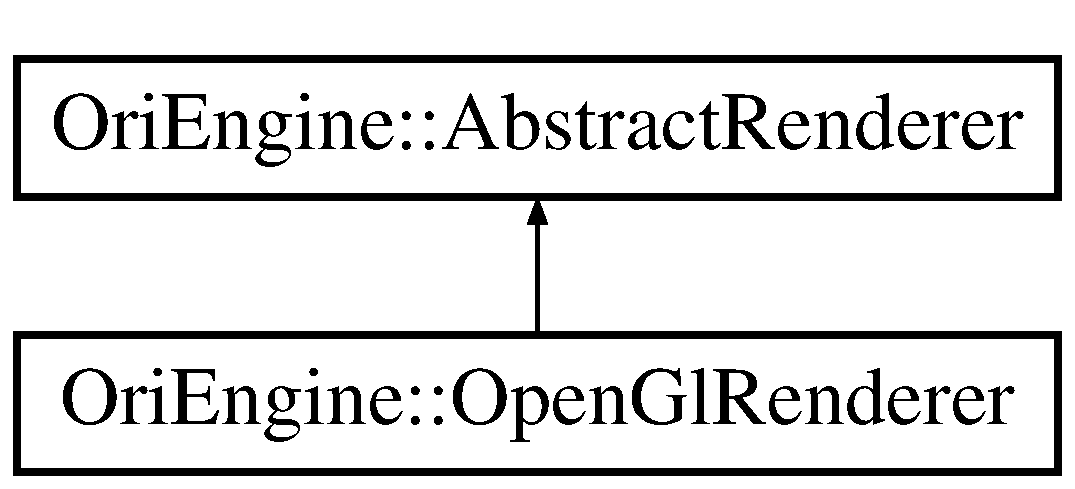
\includegraphics[height=2.000000cm]{class_ori_engine_1_1_open_gl_renderer}
\end{center}
\end{figure}
\subsection*{Public Types}
\begin{DoxyCompactItemize}
\item 
enum \hyperlink{class_ori_engine_1_1_open_gl_renderer_a2821e12392e46c549bd42b9951dbcb54}{Primative\+Type} 
\end{DoxyCompactItemize}
\subsection*{Public Member Functions}
\begin{DoxyCompactItemize}
\item 
\hyperlink{class_ori_engine_1_1_open_gl_renderer_aaa26a72feb4ccee93121b4e296184ef1}{Open\+Gl\+Renderer} ()
\item 
\hyperlink{class_ori_engine_1_1_open_gl_renderer_a184006c704765da13a684f88b355f693}{$\sim$\+Open\+Gl\+Renderer} ()
\item 
virtual void \hyperlink{class_ori_engine_1_1_open_gl_renderer_a702c4cfb099f77a04111740b9f3834e8}{init} ()
\item 
virtual void \hyperlink{class_ori_engine_1_1_open_gl_renderer_aaf6633305987ddf18d0a6e5e15e93352}{version\+Info} ()
\item 
virtual void \hyperlink{class_ori_engine_1_1_open_gl_renderer_ad75e25784e6aa3331f69b81b1b3774ff}{draw\+Primative} ()
\end{DoxyCompactItemize}


\subsection{Member Enumeration Documentation}
\hypertarget{class_ori_engine_1_1_open_gl_renderer_a2821e12392e46c549bd42b9951dbcb54}{}\label{class_ori_engine_1_1_open_gl_renderer_a2821e12392e46c549bd42b9951dbcb54} 
\index{Ori\+Engine\+::\+Open\+Gl\+Renderer@{Ori\+Engine\+::\+Open\+Gl\+Renderer}!Primative\+Type@{Primative\+Type}}
\index{Primative\+Type@{Primative\+Type}!Ori\+Engine\+::\+Open\+Gl\+Renderer@{Ori\+Engine\+::\+Open\+Gl\+Renderer}}
\subsubsection{\texorpdfstring{Primative\+Type}{PrimativeType}}
{\footnotesize\ttfamily enum \hyperlink{class_ori_engine_1_1_open_gl_renderer_a2821e12392e46c549bd42b9951dbcb54}{Ori\+Engine\+::\+Open\+Gl\+Renderer\+::\+Primative\+Type}}



\subsection{Constructor \& Destructor Documentation}
\hypertarget{class_ori_engine_1_1_open_gl_renderer_aaa26a72feb4ccee93121b4e296184ef1}{}\label{class_ori_engine_1_1_open_gl_renderer_aaa26a72feb4ccee93121b4e296184ef1} 
\index{Ori\+Engine\+::\+Open\+Gl\+Renderer@{Ori\+Engine\+::\+Open\+Gl\+Renderer}!Open\+Gl\+Renderer@{Open\+Gl\+Renderer}}
\index{Open\+Gl\+Renderer@{Open\+Gl\+Renderer}!Ori\+Engine\+::\+Open\+Gl\+Renderer@{Ori\+Engine\+::\+Open\+Gl\+Renderer}}
\subsubsection{\texorpdfstring{Open\+Gl\+Renderer()}{OpenGlRenderer()}}
{\footnotesize\ttfamily Open\+Gl\+Renderer\+::\+Open\+Gl\+Renderer (\begin{DoxyParamCaption}{ }\end{DoxyParamCaption})}

\hypertarget{class_ori_engine_1_1_open_gl_renderer_a184006c704765da13a684f88b355f693}{}\label{class_ori_engine_1_1_open_gl_renderer_a184006c704765da13a684f88b355f693} 
\index{Ori\+Engine\+::\+Open\+Gl\+Renderer@{Ori\+Engine\+::\+Open\+Gl\+Renderer}!````~Open\+Gl\+Renderer@{$\sim$\+Open\+Gl\+Renderer}}
\index{````~Open\+Gl\+Renderer@{$\sim$\+Open\+Gl\+Renderer}!Ori\+Engine\+::\+Open\+Gl\+Renderer@{Ori\+Engine\+::\+Open\+Gl\+Renderer}}
\subsubsection{\texorpdfstring{$\sim$\+Open\+Gl\+Renderer()}{~OpenGlRenderer()}}
{\footnotesize\ttfamily Open\+Gl\+Renderer\+::$\sim$\+Open\+Gl\+Renderer (\begin{DoxyParamCaption}{ }\end{DoxyParamCaption})}



\subsection{Member Function Documentation}
\hypertarget{class_ori_engine_1_1_open_gl_renderer_ad75e25784e6aa3331f69b81b1b3774ff}{}\label{class_ori_engine_1_1_open_gl_renderer_ad75e25784e6aa3331f69b81b1b3774ff} 
\index{Ori\+Engine\+::\+Open\+Gl\+Renderer@{Ori\+Engine\+::\+Open\+Gl\+Renderer}!draw\+Primative@{draw\+Primative}}
\index{draw\+Primative@{draw\+Primative}!Ori\+Engine\+::\+Open\+Gl\+Renderer@{Ori\+Engine\+::\+Open\+Gl\+Renderer}}
\subsubsection{\texorpdfstring{draw\+Primative()}{drawPrimative()}}
{\footnotesize\ttfamily void Open\+Gl\+Renderer\+::draw\+Primative (\begin{DoxyParamCaption}{ }\end{DoxyParamCaption})\hspace{0.3cm}{\ttfamily [virtual]}}



Implements \hyperlink{class_ori_engine_1_1_abstract_renderer_aece5371f0d8b99e6ee456845aba89f8d}{Ori\+Engine\+::\+Abstract\+Renderer}.

\hypertarget{class_ori_engine_1_1_open_gl_renderer_a702c4cfb099f77a04111740b9f3834e8}{}\label{class_ori_engine_1_1_open_gl_renderer_a702c4cfb099f77a04111740b9f3834e8} 
\index{Ori\+Engine\+::\+Open\+Gl\+Renderer@{Ori\+Engine\+::\+Open\+Gl\+Renderer}!init@{init}}
\index{init@{init}!Ori\+Engine\+::\+Open\+Gl\+Renderer@{Ori\+Engine\+::\+Open\+Gl\+Renderer}}
\subsubsection{\texorpdfstring{init()}{init()}}
{\footnotesize\ttfamily void Open\+Gl\+Renderer\+::init (\begin{DoxyParamCaption}{ }\end{DoxyParamCaption})\hspace{0.3cm}{\ttfamily [virtual]}}



Implements \hyperlink{class_ori_engine_1_1_abstract_renderer_a2af2aba80028b0aa4cca39097e1fdf6d}{Ori\+Engine\+::\+Abstract\+Renderer}.

\hypertarget{class_ori_engine_1_1_open_gl_renderer_aaf6633305987ddf18d0a6e5e15e93352}{}\label{class_ori_engine_1_1_open_gl_renderer_aaf6633305987ddf18d0a6e5e15e93352} 
\index{Ori\+Engine\+::\+Open\+Gl\+Renderer@{Ori\+Engine\+::\+Open\+Gl\+Renderer}!version\+Info@{version\+Info}}
\index{version\+Info@{version\+Info}!Ori\+Engine\+::\+Open\+Gl\+Renderer@{Ori\+Engine\+::\+Open\+Gl\+Renderer}}
\subsubsection{\texorpdfstring{version\+Info()}{versionInfo()}}
{\footnotesize\ttfamily void Open\+Gl\+Renderer\+::version\+Info (\begin{DoxyParamCaption}{ }\end{DoxyParamCaption})\hspace{0.3cm}{\ttfamily [virtual]}}

You can (and probably need) to get some info regarding versions and manufacturer

You can also get the version as ints 

Implements \hyperlink{class_ori_engine_1_1_abstract_renderer_a978fc31cfc5fc8c2cafa3d33367fdb32}{Ori\+Engine\+::\+Abstract\+Renderer}.



The documentation for this class was generated from the following files\+:\begin{DoxyCompactItemize}
\item 
Ori\+Engine/\+Ori\+Engine/\hyperlink{_open_gl_renderer_8h}{Open\+Gl\+Renderer.\+h}\item 
Ori\+Engine/\+Ori\+Engine/\hyperlink{_open_gl_renderer_8cpp}{Open\+Gl\+Renderer.\+cpp}\end{DoxyCompactItemize}

\hypertarget{class_ori_engine_1_1_open_g_l_renderer_builder}{}\section{Ori\+Engine\+:\+:Open\+G\+L\+Renderer\+Builder Class Reference}
\label{class_ori_engine_1_1_open_g_l_renderer_builder}\index{Ori\+Engine\+::\+Open\+G\+L\+Renderer\+Builder@{Ori\+Engine\+::\+Open\+G\+L\+Renderer\+Builder}}


{\ttfamily \#include $<$Open\+Gl\+Renderer.\+h$>$}

Inheritance diagram for Ori\+Engine\+:\+:Open\+G\+L\+Renderer\+Builder\+:\begin{figure}[H]
\begin{center}
\leavevmode
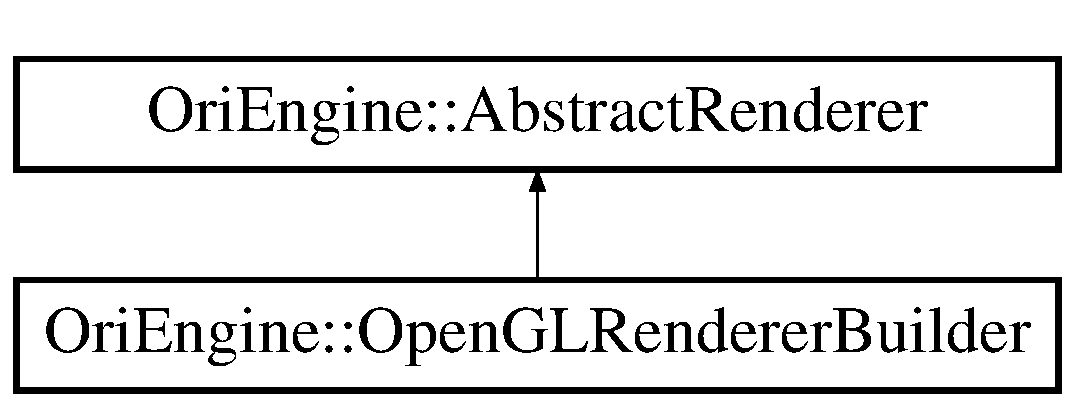
\includegraphics[height=2.000000cm]{class_ori_engine_1_1_open_g_l_renderer_builder}
\end{center}
\end{figure}
\subsection*{Public Member Functions}
\begin{DoxyCompactItemize}
\item 
virtual \hyperlink{class_ori_engine_1_1_abstract_renderer}{Abstract\+Renderer} $\ast$ \hyperlink{class_ori_engine_1_1_open_g_l_renderer_builder_a5ef23f8b0cb20f48117270819387bba9}{create\+Renderer} ()
\end{DoxyCompactItemize}


\subsection{Member Function Documentation}
\hypertarget{class_ori_engine_1_1_open_g_l_renderer_builder_a5ef23f8b0cb20f48117270819387bba9}{}\label{class_ori_engine_1_1_open_g_l_renderer_builder_a5ef23f8b0cb20f48117270819387bba9} 
\index{Ori\+Engine\+::\+Open\+G\+L\+Renderer\+Builder@{Ori\+Engine\+::\+Open\+G\+L\+Renderer\+Builder}!create\+Renderer@{create\+Renderer}}
\index{create\+Renderer@{create\+Renderer}!Ori\+Engine\+::\+Open\+G\+L\+Renderer\+Builder@{Ori\+Engine\+::\+Open\+G\+L\+Renderer\+Builder}}
\subsubsection{\texorpdfstring{create\+Renderer()}{createRenderer()}}
{\footnotesize\ttfamily virtual \hyperlink{class_ori_engine_1_1_abstract_renderer}{Abstract\+Renderer}$\ast$ Ori\+Engine\+::\+Open\+G\+L\+Renderer\+Builder\+::create\+Renderer (\begin{DoxyParamCaption}{ }\end{DoxyParamCaption})\hspace{0.3cm}{\ttfamily [virtual]}}



The documentation for this class was generated from the following file\+:\begin{DoxyCompactItemize}
\item 
Ori\+Engine/\+Ori\+Engine/\hyperlink{_open_gl_renderer_8h}{Open\+Gl\+Renderer.\+h}\end{DoxyCompactItemize}

\hypertarget{struct_ori_engine_1_1_plane}{}\section{Ori\+Engine\+:\+:Plane Struct Reference}
\label{struct_ori_engine_1_1_plane}\index{Ori\+Engine\+::\+Plane@{Ori\+Engine\+::\+Plane}}


float x,y,z; came from vector as the normal to the surface + distance to the surface (d)  




{\ttfamily \#include $<$Vector.\+h$>$}

Inheritance diagram for Ori\+Engine\+:\+:Plane\+:\begin{figure}[H]
\begin{center}
\leavevmode
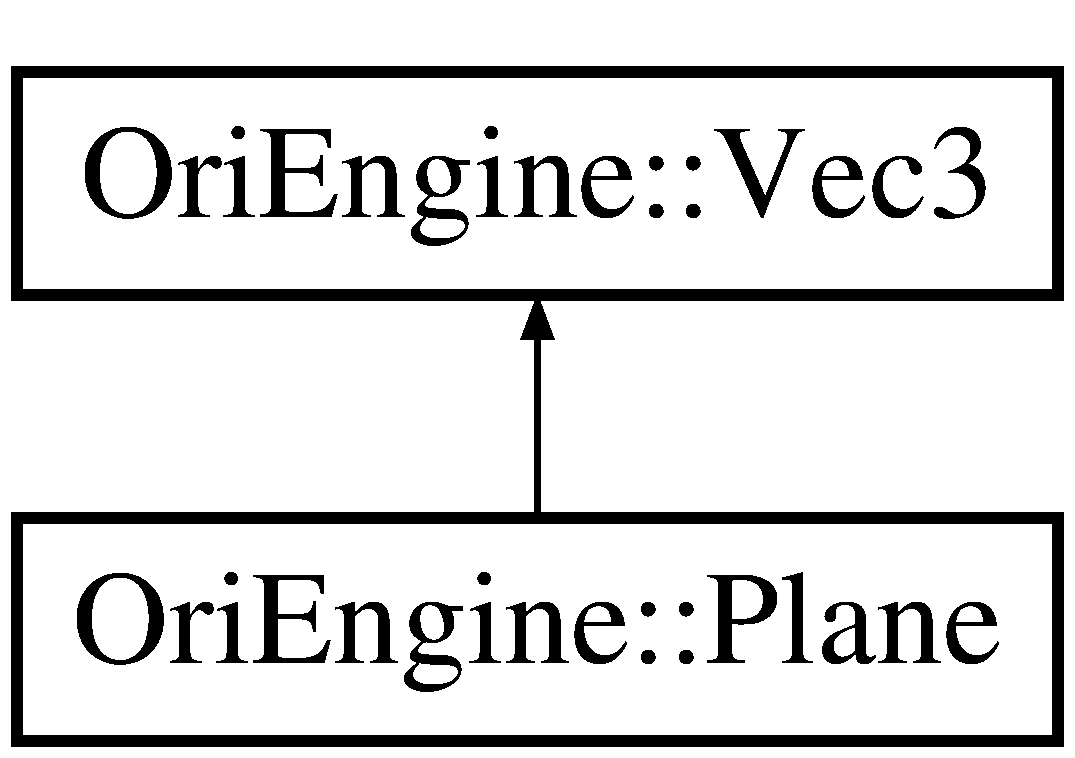
\includegraphics[height=2.000000cm]{struct_ori_engine_1_1_plane}
\end{center}
\end{figure}
\subsection*{Public Member Functions}
\begin{DoxyCompactItemize}
\item 
\hyperlink{struct_ori_engine_1_1_plane_a94deefa0a982b77ea7ad882337e06b84}{Plane} (float s=0.\+0f)
\begin{DoxyCompactList}\small\item\em Here\textquotesingle{}s a set of constructors. \end{DoxyCompactList}\item 
\hyperlink{struct_ori_engine_1_1_plane_afdd998df2694dd0861a9c5f352125a04}{Plane} (float \+\_\+x, float \+\_\+y, float \+\_\+z, float \+\_\+d)
\item 
\hyperlink{struct_ori_engine_1_1_plane_ac25785437dcaacb2adb0b3667cf78fda}{Plane} (const \hyperlink{struct_ori_engine_1_1_plane}{Plane} \&v)
\item 
\hyperlink{struct_ori_engine_1_1_plane_abffb56ba7a6f9824664be9037ebbec8c}{Plane} (const \hyperlink{struct_ori_engine_1_1_vec3}{Vec3} \&v0, const \hyperlink{struct_ori_engine_1_1_vec3}{Vec3} \&v1, const \hyperlink{struct_ori_engine_1_1_vec3}{Vec3} \&v2)
\item 
void \hyperlink{struct_ori_engine_1_1_plane_af61832e1aeaff5074e9fd035ac5b8fa4}{normalize} ()
\begin{DoxyCompactList}\small\item\em Convert this plane into a normalized plane. \end{DoxyCompactList}\item 
void \hyperlink{struct_ori_engine_1_1_plane_a607d6de04c3f0c5ea9b06cc1397f3227}{print} ()
\end{DoxyCompactItemize}
\subsection*{Public Attributes}
\begin{DoxyCompactItemize}
\item 
float \hyperlink{struct_ori_engine_1_1_plane_aa810584e42c4223d18fec10d4099a9eb}{d}
\end{DoxyCompactItemize}


\subsection{Detailed Description}
float x,y,z; came from vector as the normal to the surface + distance to the surface (d) 

\subsection{Constructor \& Destructor Documentation}
\hypertarget{struct_ori_engine_1_1_plane_a94deefa0a982b77ea7ad882337e06b84}{}\label{struct_ori_engine_1_1_plane_a94deefa0a982b77ea7ad882337e06b84} 
\index{Ori\+Engine\+::\+Plane@{Ori\+Engine\+::\+Plane}!Plane@{Plane}}
\index{Plane@{Plane}!Ori\+Engine\+::\+Plane@{Ori\+Engine\+::\+Plane}}
\subsubsection{\texorpdfstring{Plane()}{Plane()}\hspace{0.1cm}{\footnotesize\ttfamily [1/4]}}
{\footnotesize\ttfamily Ori\+Engine\+::\+Plane\+::\+Plane (\begin{DoxyParamCaption}\item[{float}]{s = {\ttfamily 0.0f} }\end{DoxyParamCaption})\hspace{0.3cm}{\ttfamily [inline]}}



Here\textquotesingle{}s a set of constructors. 

\hypertarget{struct_ori_engine_1_1_plane_afdd998df2694dd0861a9c5f352125a04}{}\label{struct_ori_engine_1_1_plane_afdd998df2694dd0861a9c5f352125a04} 
\index{Ori\+Engine\+::\+Plane@{Ori\+Engine\+::\+Plane}!Plane@{Plane}}
\index{Plane@{Plane}!Ori\+Engine\+::\+Plane@{Ori\+Engine\+::\+Plane}}
\subsubsection{\texorpdfstring{Plane()}{Plane()}\hspace{0.1cm}{\footnotesize\ttfamily [2/4]}}
{\footnotesize\ttfamily Ori\+Engine\+::\+Plane\+::\+Plane (\begin{DoxyParamCaption}\item[{float}]{\+\_\+x,  }\item[{float}]{\+\_\+y,  }\item[{float}]{\+\_\+z,  }\item[{float}]{\+\_\+d }\end{DoxyParamCaption})\hspace{0.3cm}{\ttfamily [inline]}}

\hypertarget{struct_ori_engine_1_1_plane_ac25785437dcaacb2adb0b3667cf78fda}{}\label{struct_ori_engine_1_1_plane_ac25785437dcaacb2adb0b3667cf78fda} 
\index{Ori\+Engine\+::\+Plane@{Ori\+Engine\+::\+Plane}!Plane@{Plane}}
\index{Plane@{Plane}!Ori\+Engine\+::\+Plane@{Ori\+Engine\+::\+Plane}}
\subsubsection{\texorpdfstring{Plane()}{Plane()}\hspace{0.1cm}{\footnotesize\ttfamily [3/4]}}
{\footnotesize\ttfamily Ori\+Engine\+::\+Plane\+::\+Plane (\begin{DoxyParamCaption}\item[{const \hyperlink{struct_ori_engine_1_1_plane}{Plane} \&}]{v }\end{DoxyParamCaption})\hspace{0.3cm}{\ttfamily [inline]}}

\hypertarget{struct_ori_engine_1_1_plane_abffb56ba7a6f9824664be9037ebbec8c}{}\label{struct_ori_engine_1_1_plane_abffb56ba7a6f9824664be9037ebbec8c} 
\index{Ori\+Engine\+::\+Plane@{Ori\+Engine\+::\+Plane}!Plane@{Plane}}
\index{Plane@{Plane}!Ori\+Engine\+::\+Plane@{Ori\+Engine\+::\+Plane}}
\subsubsection{\texorpdfstring{Plane()}{Plane()}\hspace{0.1cm}{\footnotesize\ttfamily [4/4]}}
{\footnotesize\ttfamily Ori\+Engine\+::\+Plane\+::\+Plane (\begin{DoxyParamCaption}\item[{const \hyperlink{struct_ori_engine_1_1_vec3}{Vec3} \&}]{v0,  }\item[{const \hyperlink{struct_ori_engine_1_1_vec3}{Vec3} \&}]{v1,  }\item[{const \hyperlink{struct_ori_engine_1_1_vec3}{Vec3} \&}]{v2 }\end{DoxyParamCaption})\hspace{0.3cm}{\ttfamily [inline]}}

This creates a normalized equation of a plane. Important\+: See note 3. This is the cross product

normalize 

\subsection{Member Function Documentation}
\hypertarget{struct_ori_engine_1_1_plane_af61832e1aeaff5074e9fd035ac5b8fa4}{}\label{struct_ori_engine_1_1_plane_af61832e1aeaff5074e9fd035ac5b8fa4} 
\index{Ori\+Engine\+::\+Plane@{Ori\+Engine\+::\+Plane}!normalize@{normalize}}
\index{normalize@{normalize}!Ori\+Engine\+::\+Plane@{Ori\+Engine\+::\+Plane}}
\subsubsection{\texorpdfstring{normalize()}{normalize()}}
{\footnotesize\ttfamily void Ori\+Engine\+::\+Plane\+::normalize (\begin{DoxyParamCaption}{ }\end{DoxyParamCaption})\hspace{0.3cm}{\ttfamily [inline]}}



Convert this plane into a normalized plane. 

\hypertarget{struct_ori_engine_1_1_plane_a607d6de04c3f0c5ea9b06cc1397f3227}{}\label{struct_ori_engine_1_1_plane_a607d6de04c3f0c5ea9b06cc1397f3227} 
\index{Ori\+Engine\+::\+Plane@{Ori\+Engine\+::\+Plane}!print@{print}}
\index{print@{print}!Ori\+Engine\+::\+Plane@{Ori\+Engine\+::\+Plane}}
\subsubsection{\texorpdfstring{print()}{print()}}
{\footnotesize\ttfamily void Ori\+Engine\+::\+Plane\+::print (\begin{DoxyParamCaption}{ }\end{DoxyParamCaption})\hspace{0.3cm}{\ttfamily [inline]}}



\subsection{Member Data Documentation}
\hypertarget{struct_ori_engine_1_1_plane_aa810584e42c4223d18fec10d4099a9eb}{}\label{struct_ori_engine_1_1_plane_aa810584e42c4223d18fec10d4099a9eb} 
\index{Ori\+Engine\+::\+Plane@{Ori\+Engine\+::\+Plane}!d@{d}}
\index{d@{d}!Ori\+Engine\+::\+Plane@{Ori\+Engine\+::\+Plane}}
\subsubsection{\texorpdfstring{d}{d}}
{\footnotesize\ttfamily float Ori\+Engine\+::\+Plane\+::d}



The documentation for this struct was generated from the following file\+:\begin{DoxyCompactItemize}
\item 
Ori\+Engine/\+Ori\+Engine/\hyperlink{_vector_8h}{Vector.\+h}\end{DoxyCompactItemize}

\hypertarget{class_skeletal_engine}{}\section{Skeletal\+Engine Class Reference}
\label{class_skeletal_engine}\index{Skeletal\+Engine@{Skeletal\+Engine}}
Inheritance diagram for Skeletal\+Engine\+:\begin{figure}[H]
\begin{center}
\leavevmode
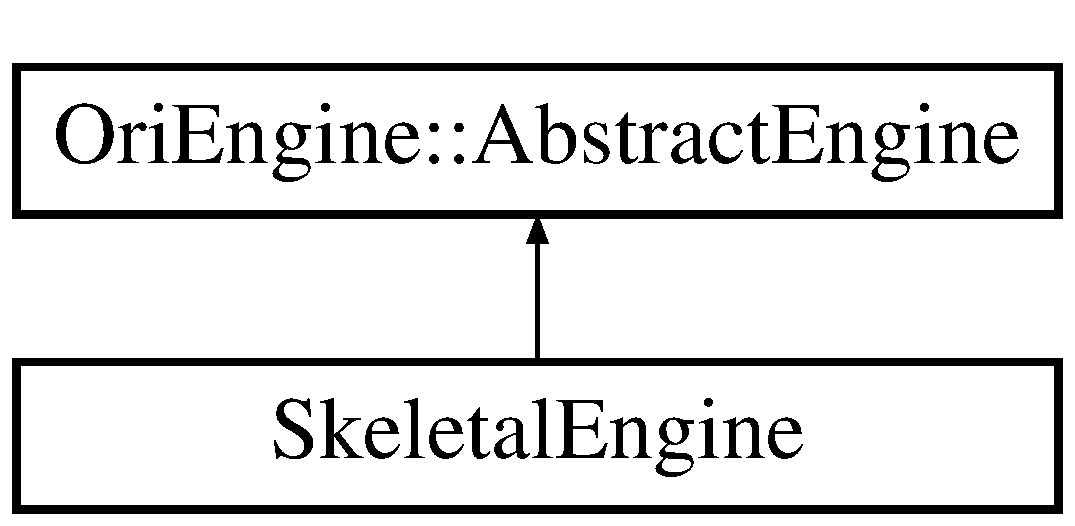
\includegraphics[height=2.000000cm]{class_skeletal_engine}
\end{center}
\end{figure}
\subsection*{Public Member Functions}
\begin{DoxyCompactItemize}
\item 
\hyperlink{class_skeletal_engine_ac12b90e475584260e9fe507ea251b79f}{Skeletal\+Engine} ()
\item 
virtual void \hyperlink{class_skeletal_engine_a58981a23dad5e0bf14aadede98bba12f}{post\+Render} ()
\item 
virtual void \hyperlink{class_skeletal_engine_ab59e698fe322bf4e600b4e3b5cf62427}{initialize\+Windowing\+System} ()
\item 
virtual void \hyperlink{class_skeletal_engine_aa947bae905c4e4628bfe5036b4943a08}{on\+Create} ()
\item 
virtual void \hyperlink{class_skeletal_engine_a9d3352322b1c4c8aa6332765e8efcde6}{pre\+Render} (double time\+Since\+Last\+Frame)
\end{DoxyCompactItemize}
\subsection*{Private Attributes}
\begin{DoxyCompactItemize}
\item 
double \hyperlink{class_skeletal_engine_a88bfb5568460595bea7d703c14e0fd97}{last\+Fps\+Print} = 0.\+0
\end{DoxyCompactItemize}
\subsection*{Additional Inherited Members}


\subsection{Constructor \& Destructor Documentation}
\hypertarget{class_skeletal_engine_ac12b90e475584260e9fe507ea251b79f}{}\label{class_skeletal_engine_ac12b90e475584260e9fe507ea251b79f} 
\index{Skeletal\+Engine@{Skeletal\+Engine}!Skeletal\+Engine@{Skeletal\+Engine}}
\index{Skeletal\+Engine@{Skeletal\+Engine}!Skeletal\+Engine@{Skeletal\+Engine}}
\subsubsection{\texorpdfstring{Skeletal\+Engine()}{SkeletalEngine()}}
{\footnotesize\ttfamily Skeletal\+Engine\+::\+Skeletal\+Engine (\begin{DoxyParamCaption}{ }\end{DoxyParamCaption})\hspace{0.3cm}{\ttfamily [inline]}}



\subsection{Member Function Documentation}
\hypertarget{class_skeletal_engine_ab59e698fe322bf4e600b4e3b5cf62427}{}\label{class_skeletal_engine_ab59e698fe322bf4e600b4e3b5cf62427} 
\index{Skeletal\+Engine@{Skeletal\+Engine}!initialize\+Windowing\+System@{initialize\+Windowing\+System}}
\index{initialize\+Windowing\+System@{initialize\+Windowing\+System}!Skeletal\+Engine@{Skeletal\+Engine}}
\subsubsection{\texorpdfstring{initialize\+Windowing\+System()}{initializeWindowingSystem()}}
{\footnotesize\ttfamily virtual void Skeletal\+Engine\+::initialize\+Windowing\+System (\begin{DoxyParamCaption}{ }\end{DoxyParamCaption})\hspace{0.3cm}{\ttfamily [inline]}, {\ttfamily [virtual]}}

\hypertarget{class_skeletal_engine_aa947bae905c4e4628bfe5036b4943a08}{}\label{class_skeletal_engine_aa947bae905c4e4628bfe5036b4943a08} 
\index{Skeletal\+Engine@{Skeletal\+Engine}!on\+Create@{on\+Create}}
\index{on\+Create@{on\+Create}!Skeletal\+Engine@{Skeletal\+Engine}}
\subsubsection{\texorpdfstring{on\+Create()}{onCreate()}}
{\footnotesize\ttfamily virtual void Skeletal\+Engine\+::on\+Create (\begin{DoxyParamCaption}{ }\end{DoxyParamCaption})\hspace{0.3cm}{\ttfamily [inline]}, {\ttfamily [virtual]}}



Implements \hyperlink{class_ori_engine_1_1_abstract_engine_a7359c90344c928e283d177159780646e}{Ori\+Engine\+::\+Abstract\+Engine}.

\hypertarget{class_skeletal_engine_a58981a23dad5e0bf14aadede98bba12f}{}\label{class_skeletal_engine_a58981a23dad5e0bf14aadede98bba12f} 
\index{Skeletal\+Engine@{Skeletal\+Engine}!post\+Render@{post\+Render}}
\index{post\+Render@{post\+Render}!Skeletal\+Engine@{Skeletal\+Engine}}
\subsubsection{\texorpdfstring{post\+Render()}{postRender()}}
{\footnotesize\ttfamily virtual void Skeletal\+Engine\+::post\+Render (\begin{DoxyParamCaption}{ }\end{DoxyParamCaption})\hspace{0.3cm}{\ttfamily [inline]}, {\ttfamily [virtual]}}



Reimplemented from \hyperlink{class_ori_engine_1_1_abstract_engine_a12ce6df5383341e36fd674a5e026bf3f}{Ori\+Engine\+::\+Abstract\+Engine}.

\hypertarget{class_skeletal_engine_a9d3352322b1c4c8aa6332765e8efcde6}{}\label{class_skeletal_engine_a9d3352322b1c4c8aa6332765e8efcde6} 
\index{Skeletal\+Engine@{Skeletal\+Engine}!pre\+Render@{pre\+Render}}
\index{pre\+Render@{pre\+Render}!Skeletal\+Engine@{Skeletal\+Engine}}
\subsubsection{\texorpdfstring{pre\+Render()}{preRender()}}
{\footnotesize\ttfamily virtual void Skeletal\+Engine\+::pre\+Render (\begin{DoxyParamCaption}\item[{double}]{time\+Since\+Last\+Frame }\end{DoxyParamCaption})\hspace{0.3cm}{\ttfamily [inline]}, {\ttfamily [virtual]}}



Reimplemented from \hyperlink{class_ori_engine_1_1_abstract_engine_a132e10c2452afe2d555ac85ea1b48845}{Ori\+Engine\+::\+Abstract\+Engine}.



\subsection{Member Data Documentation}
\hypertarget{class_skeletal_engine_a88bfb5568460595bea7d703c14e0fd97}{}\label{class_skeletal_engine_a88bfb5568460595bea7d703c14e0fd97} 
\index{Skeletal\+Engine@{Skeletal\+Engine}!last\+Fps\+Print@{last\+Fps\+Print}}
\index{last\+Fps\+Print@{last\+Fps\+Print}!Skeletal\+Engine@{Skeletal\+Engine}}
\subsubsection{\texorpdfstring{last\+Fps\+Print}{lastFpsPrint}}
{\footnotesize\ttfamily double Skeletal\+Engine\+::last\+Fps\+Print = 0.\+0\hspace{0.3cm}{\ttfamily [private]}}



The documentation for this class was generated from the following file\+:\begin{DoxyCompactItemize}
\item 
Ori\+Engine/\+Ori\+Engine/\hyperlink{_skeletal_engine_8cpp}{Skeletal\+Engine.\+cpp}\end{DoxyCompactItemize}

\hypertarget{class_ori_engine_1_1_sound}{}\section{Ori\+Engine\+:\+:Sound Class Reference}
\label{class_ori_engine_1_1_sound}\index{Ori\+Engine\+::\+Sound@{Ori\+Engine\+::\+Sound}}


{\ttfamily \#include $<$Sound.\+h$>$}

\subsection*{Public Member Functions}
\begin{DoxyCompactItemize}
\item 
\hyperlink{class_ori_engine_1_1_sound_a539c205cdf06fe2c621fd77c37bcfac9}{Sound} ()
\item 
\hyperlink{class_ori_engine_1_1_sound_a0907389078bf740be2a5763366ad3376}{$\sim$\+Sound} ()
\item 
void \hyperlink{class_ori_engine_1_1_sound_adbf1efef44994480b3c3e9becd034a7f}{load\+Sound} (const char $\ast$filename)
\item 
void \hyperlink{class_ori_engine_1_1_sound_a3ce5b74dc968ccf49b06fe1bbb22b68f}{play\+Sound} ()
\item 
void \hyperlink{class_ori_engine_1_1_sound_a2ca114ac4088d01a0fdda97fa3dc9b2b}{init} ()
\item 
void \hyperlink{class_ori_engine_1_1_sound_a1363950fc24a88df0c358f453843b80c}{update} ()
\item 
bool \hyperlink{class_ori_engine_1_1_sound_adf67b3e0608dc8e2a3e39ad92a086f8d}{get\+Channelplaying} ()
\end{DoxyCompactItemize}
\subsection*{Public Attributes}
\begin{DoxyCompactItemize}
\item 
F\+M\+O\+D\+::\+Sound $\ast$ \hyperlink{class_ori_engine_1_1_sound_a37c74fe1bf0dab55211c78a432337627}{currentsound} = 0
\item 
int \hyperlink{class_ori_engine_1_1_sound_a2836bbe85bb423313d4e5c6a8c591a44}{channelsplaying} = 0
\item 
F\+M\+O\+D\+::\+Sound $\ast$ \hyperlink{class_ori_engine_1_1_sound_a2ddb42221696bf2d74cdf3b5b560fb3e}{sound}
\item 
F\+M\+O\+D\+::\+Channel $\ast$ \hyperlink{class_ori_engine_1_1_sound_a963e5638fef3106b3715130cb1e75f82}{channel} = 0
\item 
F\+M\+O\+D\+\_\+\+R\+E\+S\+U\+LT \hyperlink{class_ori_engine_1_1_sound_ab86a49dbdac39a19e6c6aae872652d3e}{result}
\item 
unsigned int \hyperlink{class_ori_engine_1_1_sound_ac80240cf5908a2a77af263bd359b0349}{version}
\item 
void $\ast$ \hyperlink{class_ori_engine_1_1_sound_a171548ea8d26a1075cd65505688186d2}{extradriverdata} = 0
\end{DoxyCompactItemize}


\subsection{Constructor \& Destructor Documentation}
\hypertarget{class_ori_engine_1_1_sound_a539c205cdf06fe2c621fd77c37bcfac9}{}\label{class_ori_engine_1_1_sound_a539c205cdf06fe2c621fd77c37bcfac9} 
\index{Ori\+Engine\+::\+Sound@{Ori\+Engine\+::\+Sound}!Sound@{Sound}}
\index{Sound@{Sound}!Ori\+Engine\+::\+Sound@{Ori\+Engine\+::\+Sound}}
\subsubsection{\texorpdfstring{Sound()}{Sound()}}
{\footnotesize\ttfamily Sound\+::\+Sound (\begin{DoxyParamCaption}{ }\end{DoxyParamCaption})}

\hypertarget{class_ori_engine_1_1_sound_a0907389078bf740be2a5763366ad3376}{}\label{class_ori_engine_1_1_sound_a0907389078bf740be2a5763366ad3376} 
\index{Ori\+Engine\+::\+Sound@{Ori\+Engine\+::\+Sound}!````~Sound@{$\sim$\+Sound}}
\index{````~Sound@{$\sim$\+Sound}!Ori\+Engine\+::\+Sound@{Ori\+Engine\+::\+Sound}}
\subsubsection{\texorpdfstring{$\sim$\+Sound()}{~Sound()}}
{\footnotesize\ttfamily Sound\+::$\sim$\+Sound (\begin{DoxyParamCaption}{ }\end{DoxyParamCaption})}



\subsection{Member Function Documentation}
\hypertarget{class_ori_engine_1_1_sound_adf67b3e0608dc8e2a3e39ad92a086f8d}{}\label{class_ori_engine_1_1_sound_adf67b3e0608dc8e2a3e39ad92a086f8d} 
\index{Ori\+Engine\+::\+Sound@{Ori\+Engine\+::\+Sound}!get\+Channelplaying@{get\+Channelplaying}}
\index{get\+Channelplaying@{get\+Channelplaying}!Ori\+Engine\+::\+Sound@{Ori\+Engine\+::\+Sound}}
\subsubsection{\texorpdfstring{get\+Channelplaying()}{getChannelplaying()}}
{\footnotesize\ttfamily bool Sound\+::get\+Channelplaying (\begin{DoxyParamCaption}{ }\end{DoxyParamCaption})}

\hypertarget{class_ori_engine_1_1_sound_a2ca114ac4088d01a0fdda97fa3dc9b2b}{}\label{class_ori_engine_1_1_sound_a2ca114ac4088d01a0fdda97fa3dc9b2b} 
\index{Ori\+Engine\+::\+Sound@{Ori\+Engine\+::\+Sound}!init@{init}}
\index{init@{init}!Ori\+Engine\+::\+Sound@{Ori\+Engine\+::\+Sound}}
\subsubsection{\texorpdfstring{init()}{init()}}
{\footnotesize\ttfamily void Sound\+::init (\begin{DoxyParamCaption}{ }\end{DoxyParamCaption})}

\hypertarget{class_ori_engine_1_1_sound_adbf1efef44994480b3c3e9becd034a7f}{}\label{class_ori_engine_1_1_sound_adbf1efef44994480b3c3e9becd034a7f} 
\index{Ori\+Engine\+::\+Sound@{Ori\+Engine\+::\+Sound}!load\+Sound@{load\+Sound}}
\index{load\+Sound@{load\+Sound}!Ori\+Engine\+::\+Sound@{Ori\+Engine\+::\+Sound}}
\subsubsection{\texorpdfstring{load\+Sound()}{loadSound()}}
{\footnotesize\ttfamily void Sound\+::load\+Sound (\begin{DoxyParamCaption}\item[{const char $\ast$}]{filename }\end{DoxyParamCaption})}

\hypertarget{class_ori_engine_1_1_sound_a3ce5b74dc968ccf49b06fe1bbb22b68f}{}\label{class_ori_engine_1_1_sound_a3ce5b74dc968ccf49b06fe1bbb22b68f} 
\index{Ori\+Engine\+::\+Sound@{Ori\+Engine\+::\+Sound}!play\+Sound@{play\+Sound}}
\index{play\+Sound@{play\+Sound}!Ori\+Engine\+::\+Sound@{Ori\+Engine\+::\+Sound}}
\subsubsection{\texorpdfstring{play\+Sound()}{playSound()}}
{\footnotesize\ttfamily void Sound\+::play\+Sound (\begin{DoxyParamCaption}{ }\end{DoxyParamCaption})}

\hypertarget{class_ori_engine_1_1_sound_a1363950fc24a88df0c358f453843b80c}{}\label{class_ori_engine_1_1_sound_a1363950fc24a88df0c358f453843b80c} 
\index{Ori\+Engine\+::\+Sound@{Ori\+Engine\+::\+Sound}!update@{update}}
\index{update@{update}!Ori\+Engine\+::\+Sound@{Ori\+Engine\+::\+Sound}}
\subsubsection{\texorpdfstring{update()}{update()}}
{\footnotesize\ttfamily void Sound\+::update (\begin{DoxyParamCaption}{ }\end{DoxyParamCaption})}



\subsection{Member Data Documentation}
\hypertarget{class_ori_engine_1_1_sound_a963e5638fef3106b3715130cb1e75f82}{}\label{class_ori_engine_1_1_sound_a963e5638fef3106b3715130cb1e75f82} 
\index{Ori\+Engine\+::\+Sound@{Ori\+Engine\+::\+Sound}!channel@{channel}}
\index{channel@{channel}!Ori\+Engine\+::\+Sound@{Ori\+Engine\+::\+Sound}}
\subsubsection{\texorpdfstring{channel}{channel}}
{\footnotesize\ttfamily F\+M\+O\+D\+::\+Channel$\ast$ Ori\+Engine\+::\+Sound\+::channel = 0}

\hypertarget{class_ori_engine_1_1_sound_a2836bbe85bb423313d4e5c6a8c591a44}{}\label{class_ori_engine_1_1_sound_a2836bbe85bb423313d4e5c6a8c591a44} 
\index{Ori\+Engine\+::\+Sound@{Ori\+Engine\+::\+Sound}!channelsplaying@{channelsplaying}}
\index{channelsplaying@{channelsplaying}!Ori\+Engine\+::\+Sound@{Ori\+Engine\+::\+Sound}}
\subsubsection{\texorpdfstring{channelsplaying}{channelsplaying}}
{\footnotesize\ttfamily int Ori\+Engine\+::\+Sound\+::channelsplaying = 0}

\hypertarget{class_ori_engine_1_1_sound_a37c74fe1bf0dab55211c78a432337627}{}\label{class_ori_engine_1_1_sound_a37c74fe1bf0dab55211c78a432337627} 
\index{Ori\+Engine\+::\+Sound@{Ori\+Engine\+::\+Sound}!currentsound@{currentsound}}
\index{currentsound@{currentsound}!Ori\+Engine\+::\+Sound@{Ori\+Engine\+::\+Sound}}
\subsubsection{\texorpdfstring{currentsound}{currentsound}}
{\footnotesize\ttfamily F\+M\+O\+D\+::\+Sound$\ast$ Ori\+Engine\+::\+Sound\+::currentsound = 0}

\hypertarget{class_ori_engine_1_1_sound_a171548ea8d26a1075cd65505688186d2}{}\label{class_ori_engine_1_1_sound_a171548ea8d26a1075cd65505688186d2} 
\index{Ori\+Engine\+::\+Sound@{Ori\+Engine\+::\+Sound}!extradriverdata@{extradriverdata}}
\index{extradriverdata@{extradriverdata}!Ori\+Engine\+::\+Sound@{Ori\+Engine\+::\+Sound}}
\subsubsection{\texorpdfstring{extradriverdata}{extradriverdata}}
{\footnotesize\ttfamily void$\ast$ Ori\+Engine\+::\+Sound\+::extradriverdata = 0}

\hypertarget{class_ori_engine_1_1_sound_ab86a49dbdac39a19e6c6aae872652d3e}{}\label{class_ori_engine_1_1_sound_ab86a49dbdac39a19e6c6aae872652d3e} 
\index{Ori\+Engine\+::\+Sound@{Ori\+Engine\+::\+Sound}!result@{result}}
\index{result@{result}!Ori\+Engine\+::\+Sound@{Ori\+Engine\+::\+Sound}}
\subsubsection{\texorpdfstring{result}{result}}
{\footnotesize\ttfamily F\+M\+O\+D\+\_\+\+R\+E\+S\+U\+LT Ori\+Engine\+::\+Sound\+::result}

\hypertarget{class_ori_engine_1_1_sound_a2ddb42221696bf2d74cdf3b5b560fb3e}{}\label{class_ori_engine_1_1_sound_a2ddb42221696bf2d74cdf3b5b560fb3e} 
\index{Ori\+Engine\+::\+Sound@{Ori\+Engine\+::\+Sound}!sound@{sound}}
\index{sound@{sound}!Ori\+Engine\+::\+Sound@{Ori\+Engine\+::\+Sound}}
\subsubsection{\texorpdfstring{sound}{sound}}
{\footnotesize\ttfamily F\+M\+O\+D\+::\+Sound$\ast$ Ori\+Engine\+::\+Sound\+::sound}

\hypertarget{class_ori_engine_1_1_sound_ac80240cf5908a2a77af263bd359b0349}{}\label{class_ori_engine_1_1_sound_ac80240cf5908a2a77af263bd359b0349} 
\index{Ori\+Engine\+::\+Sound@{Ori\+Engine\+::\+Sound}!version@{version}}
\index{version@{version}!Ori\+Engine\+::\+Sound@{Ori\+Engine\+::\+Sound}}
\subsubsection{\texorpdfstring{version}{version}}
{\footnotesize\ttfamily unsigned int Ori\+Engine\+::\+Sound\+::version}



The documentation for this class was generated from the following files\+:\begin{DoxyCompactItemize}
\item 
Ori\+Engine/\+Ori\+Engine/\hyperlink{_sound_8h}{Sound.\+h}\item 
Ori\+Engine/\+Ori\+Engine/\hyperlink{_sound_8cpp}{Sound.\+cpp}\end{DoxyCompactItemize}

\hypertarget{class_ori_engine_1_1_sound_manager}{}\section{Ori\+Engine\+:\+:Sound\+Manager Class Reference}
\label{class_ori_engine_1_1_sound_manager}\index{Ori\+Engine\+::\+Sound\+Manager@{Ori\+Engine\+::\+Sound\+Manager}}


{\ttfamily \#include $<$Sound\+Manager.\+h$>$}

\subsection*{Public Member Functions}
\begin{DoxyCompactItemize}
\item 
\hyperlink{class_ori_engine_1_1_sound_manager_abcc1fbf3488be5788a42c9a4fe56df35}{Sound\+Manager} ()
\item 
\hyperlink{class_ori_engine_1_1_sound_manager_ad5dbf8eab22db48ff8f3db51b02f8938}{$\sim$\+Sound\+Manager} ()
\item 
void \hyperlink{class_ori_engine_1_1_sound_manager_a489e924e813bb17f740dfd4605599baa}{load\+Soundby\+Index} (char $\ast$filename, int index)
\item 
void \hyperlink{class_ori_engine_1_1_sound_manager_add98e983ee46bd07c790503339b87933}{play\+Soundby\+Index} (int index)
\item 
void \hyperlink{class_ori_engine_1_1_sound_manager_a5492c808a16860c1a04f9ad1309b0b91}{stop\+Soundby\+Index} (int index)
\item 
void \hyperlink{class_ori_engine_1_1_sound_manager_a6fbde6d8a9b132fea206fcfb4dd35990}{init} ()
\item 
void \hyperlink{class_ori_engine_1_1_sound_manager_a5da083b0b4feb1ae9c3c86823d5be196}{update\+Sound} (int index)
\end{DoxyCompactItemize}
\subsection*{Public Attributes}
\begin{DoxyCompactItemize}
\item 
std\+::vector$<$ \hyperlink{class_ori_engine_1_1_sound}{Sound} $>$ \hyperlink{class_ori_engine_1_1_sound_manager_a241dbad02456e387d20aa32694d8c5eb}{sounds}
\item 
\hyperlink{class_ori_engine_1_1_system}{System} \hyperlink{class_ori_engine_1_1_sound_manager_a0530694c6def60abba7c82da657b5398}{system}
\end{DoxyCompactItemize}


\subsection{Constructor \& Destructor Documentation}
\hypertarget{class_ori_engine_1_1_sound_manager_abcc1fbf3488be5788a42c9a4fe56df35}{}\label{class_ori_engine_1_1_sound_manager_abcc1fbf3488be5788a42c9a4fe56df35} 
\index{Ori\+Engine\+::\+Sound\+Manager@{Ori\+Engine\+::\+Sound\+Manager}!Sound\+Manager@{Sound\+Manager}}
\index{Sound\+Manager@{Sound\+Manager}!Ori\+Engine\+::\+Sound\+Manager@{Ori\+Engine\+::\+Sound\+Manager}}
\subsubsection{\texorpdfstring{Sound\+Manager()}{SoundManager()}}
{\footnotesize\ttfamily Sound\+Manager\+::\+Sound\+Manager (\begin{DoxyParamCaption}{ }\end{DoxyParamCaption})}

\hypertarget{class_ori_engine_1_1_sound_manager_ad5dbf8eab22db48ff8f3db51b02f8938}{}\label{class_ori_engine_1_1_sound_manager_ad5dbf8eab22db48ff8f3db51b02f8938} 
\index{Ori\+Engine\+::\+Sound\+Manager@{Ori\+Engine\+::\+Sound\+Manager}!````~Sound\+Manager@{$\sim$\+Sound\+Manager}}
\index{````~Sound\+Manager@{$\sim$\+Sound\+Manager}!Ori\+Engine\+::\+Sound\+Manager@{Ori\+Engine\+::\+Sound\+Manager}}
\subsubsection{\texorpdfstring{$\sim$\+Sound\+Manager()}{~SoundManager()}}
{\footnotesize\ttfamily Sound\+Manager\+::$\sim$\+Sound\+Manager (\begin{DoxyParamCaption}{ }\end{DoxyParamCaption})}



\subsection{Member Function Documentation}
\hypertarget{class_ori_engine_1_1_sound_manager_a6fbde6d8a9b132fea206fcfb4dd35990}{}\label{class_ori_engine_1_1_sound_manager_a6fbde6d8a9b132fea206fcfb4dd35990} 
\index{Ori\+Engine\+::\+Sound\+Manager@{Ori\+Engine\+::\+Sound\+Manager}!init@{init}}
\index{init@{init}!Ori\+Engine\+::\+Sound\+Manager@{Ori\+Engine\+::\+Sound\+Manager}}
\subsubsection{\texorpdfstring{init()}{init()}}
{\footnotesize\ttfamily void Ori\+Engine\+::\+Sound\+Manager\+::init (\begin{DoxyParamCaption}{ }\end{DoxyParamCaption})}

\hypertarget{class_ori_engine_1_1_sound_manager_a489e924e813bb17f740dfd4605599baa}{}\label{class_ori_engine_1_1_sound_manager_a489e924e813bb17f740dfd4605599baa} 
\index{Ori\+Engine\+::\+Sound\+Manager@{Ori\+Engine\+::\+Sound\+Manager}!load\+Soundby\+Index@{load\+Soundby\+Index}}
\index{load\+Soundby\+Index@{load\+Soundby\+Index}!Ori\+Engine\+::\+Sound\+Manager@{Ori\+Engine\+::\+Sound\+Manager}}
\subsubsection{\texorpdfstring{load\+Soundby\+Index()}{loadSoundbyIndex()}}
{\footnotesize\ttfamily void Sound\+Manager\+::load\+Soundby\+Index (\begin{DoxyParamCaption}\item[{char $\ast$}]{filename,  }\item[{int}]{index }\end{DoxyParamCaption})}

\hypertarget{class_ori_engine_1_1_sound_manager_add98e983ee46bd07c790503339b87933}{}\label{class_ori_engine_1_1_sound_manager_add98e983ee46bd07c790503339b87933} 
\index{Ori\+Engine\+::\+Sound\+Manager@{Ori\+Engine\+::\+Sound\+Manager}!play\+Soundby\+Index@{play\+Soundby\+Index}}
\index{play\+Soundby\+Index@{play\+Soundby\+Index}!Ori\+Engine\+::\+Sound\+Manager@{Ori\+Engine\+::\+Sound\+Manager}}
\subsubsection{\texorpdfstring{play\+Soundby\+Index()}{playSoundbyIndex()}}
{\footnotesize\ttfamily void Sound\+Manager\+::play\+Soundby\+Index (\begin{DoxyParamCaption}\item[{int}]{index }\end{DoxyParamCaption})}

\hypertarget{class_ori_engine_1_1_sound_manager_a5492c808a16860c1a04f9ad1309b0b91}{}\label{class_ori_engine_1_1_sound_manager_a5492c808a16860c1a04f9ad1309b0b91} 
\index{Ori\+Engine\+::\+Sound\+Manager@{Ori\+Engine\+::\+Sound\+Manager}!stop\+Soundby\+Index@{stop\+Soundby\+Index}}
\index{stop\+Soundby\+Index@{stop\+Soundby\+Index}!Ori\+Engine\+::\+Sound\+Manager@{Ori\+Engine\+::\+Sound\+Manager}}
\subsubsection{\texorpdfstring{stop\+Soundby\+Index()}{stopSoundbyIndex()}}
{\footnotesize\ttfamily void Sound\+Manager\+::stop\+Soundby\+Index (\begin{DoxyParamCaption}\item[{int}]{index }\end{DoxyParamCaption})}

\hypertarget{class_ori_engine_1_1_sound_manager_a5da083b0b4feb1ae9c3c86823d5be196}{}\label{class_ori_engine_1_1_sound_manager_a5da083b0b4feb1ae9c3c86823d5be196} 
\index{Ori\+Engine\+::\+Sound\+Manager@{Ori\+Engine\+::\+Sound\+Manager}!update\+Sound@{update\+Sound}}
\index{update\+Sound@{update\+Sound}!Ori\+Engine\+::\+Sound\+Manager@{Ori\+Engine\+::\+Sound\+Manager}}
\subsubsection{\texorpdfstring{update\+Sound()}{updateSound()}}
{\footnotesize\ttfamily void Sound\+Manager\+::update\+Sound (\begin{DoxyParamCaption}\item[{int}]{index }\end{DoxyParamCaption})}



\subsection{Member Data Documentation}
\hypertarget{class_ori_engine_1_1_sound_manager_a241dbad02456e387d20aa32694d8c5eb}{}\label{class_ori_engine_1_1_sound_manager_a241dbad02456e387d20aa32694d8c5eb} 
\index{Ori\+Engine\+::\+Sound\+Manager@{Ori\+Engine\+::\+Sound\+Manager}!sounds@{sounds}}
\index{sounds@{sounds}!Ori\+Engine\+::\+Sound\+Manager@{Ori\+Engine\+::\+Sound\+Manager}}
\subsubsection{\texorpdfstring{sounds}{sounds}}
{\footnotesize\ttfamily std\+::vector$<$\hyperlink{class_ori_engine_1_1_sound}{Sound}$>$ Ori\+Engine\+::\+Sound\+Manager\+::sounds}

\hypertarget{class_ori_engine_1_1_sound_manager_a0530694c6def60abba7c82da657b5398}{}\label{class_ori_engine_1_1_sound_manager_a0530694c6def60abba7c82da657b5398} 
\index{Ori\+Engine\+::\+Sound\+Manager@{Ori\+Engine\+::\+Sound\+Manager}!system@{system}}
\index{system@{system}!Ori\+Engine\+::\+Sound\+Manager@{Ori\+Engine\+::\+Sound\+Manager}}
\subsubsection{\texorpdfstring{system}{system}}
{\footnotesize\ttfamily \hyperlink{class_ori_engine_1_1_system}{System} Ori\+Engine\+::\+Sound\+Manager\+::system}



The documentation for this class was generated from the following files\+:\begin{DoxyCompactItemize}
\item 
Ori\+Engine/\+Ori\+Engine/\hyperlink{_sound_manager_8h}{Sound\+Manager.\+h}\item 
Ori\+Engine/\+Ori\+Engine/\hyperlink{_sound_manager_8cpp}{Sound\+Manager.\+cpp}\end{DoxyCompactItemize}

\hypertarget{struct_ori_engine_1_1_sphere}{}\section{Ori\+Engine\+:\+:Sphere Struct Reference}
\label{struct_ori_engine_1_1_sphere}\index{Ori\+Engine\+::\+Sphere@{Ori\+Engine\+::\+Sphere}}


Just some extra stuff for fun.  




{\ttfamily \#include $<$Vector.\+h$>$}

Inheritance diagram for Ori\+Engine\+:\+:Sphere\+:\begin{figure}[H]
\begin{center}
\leavevmode
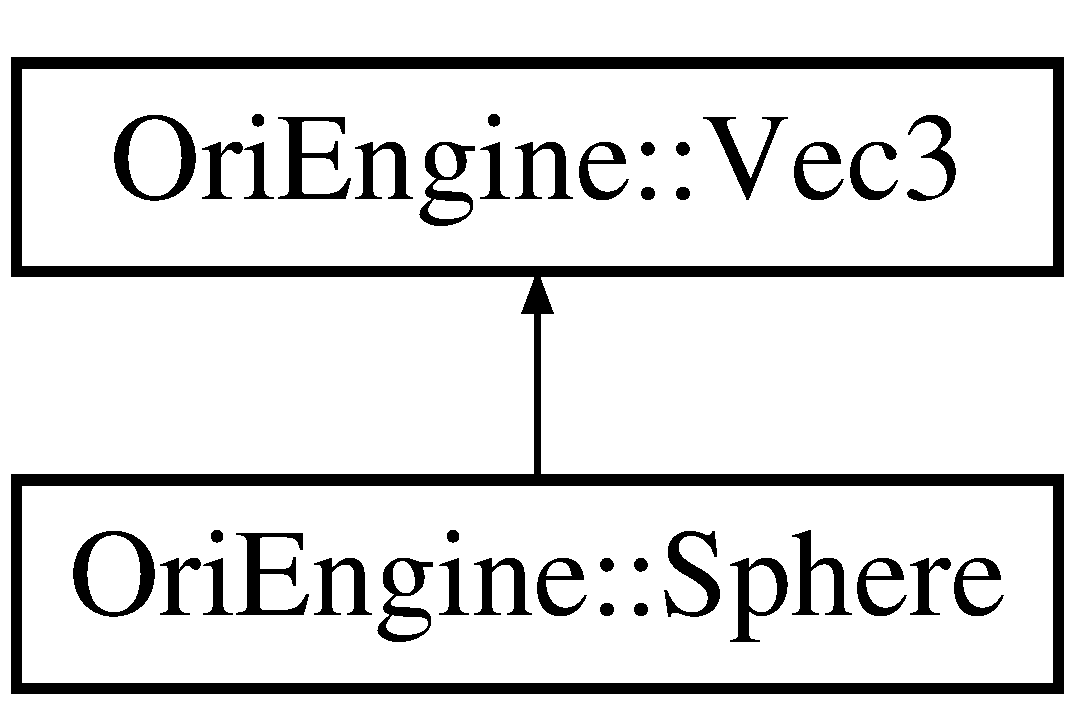
\includegraphics[height=2.000000cm]{struct_ori_engine_1_1_sphere}
\end{center}
\end{figure}
\subsection*{Public Member Functions}
\begin{DoxyCompactItemize}
\item 
\hyperlink{struct_ori_engine_1_1_sphere_ac20aefe7563c0713c9ff1129887437fd}{Sphere} (float s=0.\+0f)
\item 
\hyperlink{struct_ori_engine_1_1_sphere_ad2abc0c7e4786dcf29394b30cbeca2dd}{Sphere} (float \+\_\+x, float \+\_\+y, float \+\_\+z, float \+\_\+r)
\item 
\hyperlink{struct_ori_engine_1_1_sphere_aaff2b5e8886e1a2e4b17b0e615c1f2e7}{Sphere} (const \hyperlink{struct_ori_engine_1_1_sphere}{Sphere} \&v)
\item 
void \hyperlink{struct_ori_engine_1_1_sphere_a35400ef1bae1de87d1ccc6dfe9b3b5be}{print} ()
\end{DoxyCompactItemize}
\subsection*{Public Attributes}
\begin{DoxyCompactItemize}
\item 
float \hyperlink{struct_ori_engine_1_1_sphere_a24c8eda50b041688fd57b2b3c1305726}{r}
\end{DoxyCompactItemize}


\subsection{Detailed Description}
Just some extra stuff for fun. 

A \hyperlink{struct_ori_engine_1_1_sphere}{Sphere} could be thought of as a just a center point (x,y,z) comes from \hyperlink{struct_ori_engine_1_1_vec3}{Vec3} then just add a radius 

\subsection{Constructor \& Destructor Documentation}
\hypertarget{struct_ori_engine_1_1_sphere_ac20aefe7563c0713c9ff1129887437fd}{}\label{struct_ori_engine_1_1_sphere_ac20aefe7563c0713c9ff1129887437fd} 
\index{Ori\+Engine\+::\+Sphere@{Ori\+Engine\+::\+Sphere}!Sphere@{Sphere}}
\index{Sphere@{Sphere}!Ori\+Engine\+::\+Sphere@{Ori\+Engine\+::\+Sphere}}
\subsubsection{\texorpdfstring{Sphere()}{Sphere()}\hspace{0.1cm}{\footnotesize\ttfamily [1/3]}}
{\footnotesize\ttfamily Ori\+Engine\+::\+Sphere\+::\+Sphere (\begin{DoxyParamCaption}\item[{float}]{s = {\ttfamily 0.0f} }\end{DoxyParamCaption})\hspace{0.3cm}{\ttfamily [inline]}}

\hypertarget{struct_ori_engine_1_1_sphere_ad2abc0c7e4786dcf29394b30cbeca2dd}{}\label{struct_ori_engine_1_1_sphere_ad2abc0c7e4786dcf29394b30cbeca2dd} 
\index{Ori\+Engine\+::\+Sphere@{Ori\+Engine\+::\+Sphere}!Sphere@{Sphere}}
\index{Sphere@{Sphere}!Ori\+Engine\+::\+Sphere@{Ori\+Engine\+::\+Sphere}}
\subsubsection{\texorpdfstring{Sphere()}{Sphere()}\hspace{0.1cm}{\footnotesize\ttfamily [2/3]}}
{\footnotesize\ttfamily Ori\+Engine\+::\+Sphere\+::\+Sphere (\begin{DoxyParamCaption}\item[{float}]{\+\_\+x,  }\item[{float}]{\+\_\+y,  }\item[{float}]{\+\_\+z,  }\item[{float}]{\+\_\+r }\end{DoxyParamCaption})\hspace{0.3cm}{\ttfamily [inline]}}

\hypertarget{struct_ori_engine_1_1_sphere_aaff2b5e8886e1a2e4b17b0e615c1f2e7}{}\label{struct_ori_engine_1_1_sphere_aaff2b5e8886e1a2e4b17b0e615c1f2e7} 
\index{Ori\+Engine\+::\+Sphere@{Ori\+Engine\+::\+Sphere}!Sphere@{Sphere}}
\index{Sphere@{Sphere}!Ori\+Engine\+::\+Sphere@{Ori\+Engine\+::\+Sphere}}
\subsubsection{\texorpdfstring{Sphere()}{Sphere()}\hspace{0.1cm}{\footnotesize\ttfamily [3/3]}}
{\footnotesize\ttfamily Ori\+Engine\+::\+Sphere\+::\+Sphere (\begin{DoxyParamCaption}\item[{const \hyperlink{struct_ori_engine_1_1_sphere}{Sphere} \&}]{v }\end{DoxyParamCaption})\hspace{0.3cm}{\ttfamily [inline]}}



\subsection{Member Function Documentation}
\hypertarget{struct_ori_engine_1_1_sphere_a35400ef1bae1de87d1ccc6dfe9b3b5be}{}\label{struct_ori_engine_1_1_sphere_a35400ef1bae1de87d1ccc6dfe9b3b5be} 
\index{Ori\+Engine\+::\+Sphere@{Ori\+Engine\+::\+Sphere}!print@{print}}
\index{print@{print}!Ori\+Engine\+::\+Sphere@{Ori\+Engine\+::\+Sphere}}
\subsubsection{\texorpdfstring{print()}{print()}}
{\footnotesize\ttfamily void Ori\+Engine\+::\+Sphere\+::print (\begin{DoxyParamCaption}{ }\end{DoxyParamCaption})\hspace{0.3cm}{\ttfamily [inline]}}



\subsection{Member Data Documentation}
\hypertarget{struct_ori_engine_1_1_sphere_a24c8eda50b041688fd57b2b3c1305726}{}\label{struct_ori_engine_1_1_sphere_a24c8eda50b041688fd57b2b3c1305726} 
\index{Ori\+Engine\+::\+Sphere@{Ori\+Engine\+::\+Sphere}!r@{r}}
\index{r@{r}!Ori\+Engine\+::\+Sphere@{Ori\+Engine\+::\+Sphere}}
\subsubsection{\texorpdfstring{r}{r}}
{\footnotesize\ttfamily float Ori\+Engine\+::\+Sphere\+::r}



The documentation for this struct was generated from the following file\+:\begin{DoxyCompactItemize}
\item 
Ori\+Engine/\+Ori\+Engine/\hyperlink{_vector_8h}{Vector.\+h}\end{DoxyCompactItemize}

\hypertarget{class_ori_engine_1_1_system}{}\section{Ori\+Engine\+:\+:System Class Reference}
\label{class_ori_engine_1_1_system}\index{Ori\+Engine\+::\+System@{Ori\+Engine\+::\+System}}


{\ttfamily \#include $<$Sound.\+h$>$}

\subsection*{Private Attributes}
\begin{DoxyCompactItemize}
\item 
F\+M\+O\+D\+::\+System $\ast$ \hyperlink{class_ori_engine_1_1_system_a1b2c7b3a05848016f765c4342ec27a45}{system}
\end{DoxyCompactItemize}


\subsection{Member Data Documentation}
\hypertarget{class_ori_engine_1_1_system_a1b2c7b3a05848016f765c4342ec27a45}{}\label{class_ori_engine_1_1_system_a1b2c7b3a05848016f765c4342ec27a45} 
\index{Ori\+Engine\+::\+System@{Ori\+Engine\+::\+System}!system@{system}}
\index{system@{system}!Ori\+Engine\+::\+System@{Ori\+Engine\+::\+System}}
\subsubsection{\texorpdfstring{system}{system}}
{\footnotesize\ttfamily F\+M\+O\+D\+::\+System$\ast$ Ori\+Engine\+::\+System\+::system\hspace{0.3cm}{\ttfamily [private]}}



The documentation for this class was generated from the following file\+:\begin{DoxyCompactItemize}
\item 
Ori\+Engine/\+Ori\+Engine/\hyperlink{_sound_8h}{Sound.\+h}\end{DoxyCompactItemize}

\hypertarget{struct_ori_engine_1_1_vec2}{}\section{Ori\+Engine\+:\+:Vec2 Struct Reference}
\label{struct_ori_engine_1_1_vec2}\index{Ori\+Engine\+::\+Vec2@{Ori\+Engine\+::\+Vec2}}


{\ttfamily \#include $<$Vector.\+h$>$}

\subsection*{Public Member Functions}
\begin{DoxyCompactItemize}
\item 
void \hyperlink{struct_ori_engine_1_1_vec2_af08ea6c4eedd4b37fe25815f3555015e}{Vec2\+::\+Load} (float \+\_\+x, float \+\_\+y)
\begin{DoxyCompactList}\small\item\em Structures are default public! \end{DoxyCompactList}\item 
\hyperlink{struct_ori_engine_1_1_vec2_a115419a0f94d31618b93c03be1117089}{Vec2} (float s=float(0.\+0))
\begin{DoxyCompactList}\small\item\em Here\textquotesingle{}s a set of constructors. \end{DoxyCompactList}\item 
\hyperlink{struct_ori_engine_1_1_vec2_a3f324decdc2b86e4a498a95e706f4c20}{Vec2} (float \+\_\+x, float \+\_\+y)
\item 
\hyperlink{struct_ori_engine_1_1_vec2_a8769147a1ce655442d97dbeb504151a7}{Vec2} (const \hyperlink{struct_ori_engine_1_1_vec2}{Vec2} \&v)
\begin{DoxyCompactList}\small\item\em In this context \char`\"{}const\char`\"{} means I promise not to modify anything v points to. \end{DoxyCompactList}\item 
const float \hyperlink{struct_ori_engine_1_1_vec2_a481efce1521eb8c44802275f56030ea5}{operator\mbox{[}$\,$\mbox{]}} (int index) const
\begin{DoxyCompactList}\small\item\em Now we can use the \hyperlink{struct_ori_engine_1_1_vec2}{Vec2} like an array but we\textquotesingle{}ll need two overloads. \end{DoxyCompactList}\item 
float \& \hyperlink{struct_ori_engine_1_1_vec2_a80dd5e430ccf80c1e7cac25da0262a8d}{operator\mbox{[}$\,$\mbox{]}} (int index)
\end{DoxyCompactItemize}
\subsection*{Public Attributes}
\begin{DoxyCompactItemize}
\item 
float \hyperlink{struct_ori_engine_1_1_vec2_a03d48413df5d90b9985f677b255e7135}{x}
\begin{DoxyCompactList}\small\item\em Someone is going to want this someday. \end{DoxyCompactList}\item 
float \hyperlink{struct_ori_engine_1_1_vec2_a0fb55c74edfbbc37c84004c8cb3a18dc}{y}
\end{DoxyCompactItemize}


\subsection{Constructor \& Destructor Documentation}
\hypertarget{struct_ori_engine_1_1_vec2_a115419a0f94d31618b93c03be1117089}{}\label{struct_ori_engine_1_1_vec2_a115419a0f94d31618b93c03be1117089} 
\index{Ori\+Engine\+::\+Vec2@{Ori\+Engine\+::\+Vec2}!Vec2@{Vec2}}
\index{Vec2@{Vec2}!Ori\+Engine\+::\+Vec2@{Ori\+Engine\+::\+Vec2}}
\subsubsection{\texorpdfstring{Vec2()}{Vec2()}\hspace{0.1cm}{\footnotesize\ttfamily [1/3]}}
{\footnotesize\ttfamily Ori\+Engine\+::\+Vec2\+::\+Vec2 (\begin{DoxyParamCaption}\item[{float}]{s = {\ttfamily float(0.0)} }\end{DoxyParamCaption})\hspace{0.3cm}{\ttfamily [inline]}}



Here\textquotesingle{}s a set of constructors. 

\hypertarget{struct_ori_engine_1_1_vec2_a3f324decdc2b86e4a498a95e706f4c20}{}\label{struct_ori_engine_1_1_vec2_a3f324decdc2b86e4a498a95e706f4c20} 
\index{Ori\+Engine\+::\+Vec2@{Ori\+Engine\+::\+Vec2}!Vec2@{Vec2}}
\index{Vec2@{Vec2}!Ori\+Engine\+::\+Vec2@{Ori\+Engine\+::\+Vec2}}
\subsubsection{\texorpdfstring{Vec2()}{Vec2()}\hspace{0.1cm}{\footnotesize\ttfamily [2/3]}}
{\footnotesize\ttfamily Ori\+Engine\+::\+Vec2\+::\+Vec2 (\begin{DoxyParamCaption}\item[{float}]{\+\_\+x,  }\item[{float}]{\+\_\+y }\end{DoxyParamCaption})\hspace{0.3cm}{\ttfamily [inline]}}

\hypertarget{struct_ori_engine_1_1_vec2_a8769147a1ce655442d97dbeb504151a7}{}\label{struct_ori_engine_1_1_vec2_a8769147a1ce655442d97dbeb504151a7} 
\index{Ori\+Engine\+::\+Vec2@{Ori\+Engine\+::\+Vec2}!Vec2@{Vec2}}
\index{Vec2@{Vec2}!Ori\+Engine\+::\+Vec2@{Ori\+Engine\+::\+Vec2}}
\subsubsection{\texorpdfstring{Vec2()}{Vec2()}\hspace{0.1cm}{\footnotesize\ttfamily [3/3]}}
{\footnotesize\ttfamily Ori\+Engine\+::\+Vec2\+::\+Vec2 (\begin{DoxyParamCaption}\item[{const \hyperlink{struct_ori_engine_1_1_vec2}{Vec2} \&}]{v }\end{DoxyParamCaption})\hspace{0.3cm}{\ttfamily [inline]}}



In this context \char`\"{}const\char`\"{} means I promise not to modify anything v points to. 



\subsection{Member Function Documentation}
\hypertarget{struct_ori_engine_1_1_vec2_a481efce1521eb8c44802275f56030ea5}{}\label{struct_ori_engine_1_1_vec2_a481efce1521eb8c44802275f56030ea5} 
\index{Ori\+Engine\+::\+Vec2@{Ori\+Engine\+::\+Vec2}!operator\mbox{[}\mbox{]}@{operator[]}}
\index{operator\mbox{[}\mbox{]}@{operator[]}!Ori\+Engine\+::\+Vec2@{Ori\+Engine\+::\+Vec2}}
\subsubsection{\texorpdfstring{operator[]()}{operator[]()}\hspace{0.1cm}{\footnotesize\ttfamily [1/2]}}
{\footnotesize\ttfamily const float Ori\+Engine\+::\+Vec2\+::operator\mbox{[}$\,$\mbox{]} (\begin{DoxyParamCaption}\item[{int}]{index }\end{DoxyParamCaption}) const\hspace{0.3cm}{\ttfamily [inline]}}



Now we can use the \hyperlink{struct_ori_engine_1_1_vec2}{Vec2} like an array but we\textquotesingle{}ll need two overloads. 

This one is for reading the \hyperlink{struct_ori_engine_1_1_vec3}{Vec3} as if where an array \hypertarget{struct_ori_engine_1_1_vec2_a80dd5e430ccf80c1e7cac25da0262a8d}{}\label{struct_ori_engine_1_1_vec2_a80dd5e430ccf80c1e7cac25da0262a8d} 
\index{Ori\+Engine\+::\+Vec2@{Ori\+Engine\+::\+Vec2}!operator\mbox{[}\mbox{]}@{operator[]}}
\index{operator\mbox{[}\mbox{]}@{operator[]}!Ori\+Engine\+::\+Vec2@{Ori\+Engine\+::\+Vec2}}
\subsubsection{\texorpdfstring{operator[]()}{operator[]()}\hspace{0.1cm}{\footnotesize\ttfamily [2/2]}}
{\footnotesize\ttfamily float\& Ori\+Engine\+::\+Vec2\+::operator\mbox{[}$\,$\mbox{]} (\begin{DoxyParamCaption}\item[{int}]{index }\end{DoxyParamCaption})\hspace{0.3cm}{\ttfamily [inline]}}

This one is for writing to the \hyperlink{struct_ori_engine_1_1_vec2}{Vec2} as if where an array -\/ check out the term lvalue \hypertarget{struct_ori_engine_1_1_vec2_af08ea6c4eedd4b37fe25815f3555015e}{}\label{struct_ori_engine_1_1_vec2_af08ea6c4eedd4b37fe25815f3555015e} 
\index{Ori\+Engine\+::\+Vec2@{Ori\+Engine\+::\+Vec2}!Vec2\+::\+Load@{Vec2\+::\+Load}}
\index{Vec2\+::\+Load@{Vec2\+::\+Load}!Ori\+Engine\+::\+Vec2@{Ori\+Engine\+::\+Vec2}}
\subsubsection{\texorpdfstring{Vec2\+::\+Load()}{Vec2::Load()}}
{\footnotesize\ttfamily void Ori\+Engine\+::\+Vec2\+::\+Vec2\+::\+Load (\begin{DoxyParamCaption}\item[{float}]{\+\_\+x,  }\item[{float}]{\+\_\+y }\end{DoxyParamCaption})\hspace{0.3cm}{\ttfamily [inline]}}



Structures are default public! 



\subsection{Member Data Documentation}
\hypertarget{struct_ori_engine_1_1_vec2_a03d48413df5d90b9985f677b255e7135}{}\label{struct_ori_engine_1_1_vec2_a03d48413df5d90b9985f677b255e7135} 
\index{Ori\+Engine\+::\+Vec2@{Ori\+Engine\+::\+Vec2}!x@{x}}
\index{x@{x}!Ori\+Engine\+::\+Vec2@{Ori\+Engine\+::\+Vec2}}
\subsubsection{\texorpdfstring{x}{x}}
{\footnotesize\ttfamily float Ori\+Engine\+::\+Vec2\+::x}



Someone is going to want this someday. 

\hypertarget{struct_ori_engine_1_1_vec2_a0fb55c74edfbbc37c84004c8cb3a18dc}{}\label{struct_ori_engine_1_1_vec2_a0fb55c74edfbbc37c84004c8cb3a18dc} 
\index{Ori\+Engine\+::\+Vec2@{Ori\+Engine\+::\+Vec2}!y@{y}}
\index{y@{y}!Ori\+Engine\+::\+Vec2@{Ori\+Engine\+::\+Vec2}}
\subsubsection{\texorpdfstring{y}{y}}
{\footnotesize\ttfamily float Ori\+Engine\+::\+Vec2\+::y}



The documentation for this struct was generated from the following file\+:\begin{DoxyCompactItemize}
\item 
Ori\+Engine/\+Ori\+Engine/\hyperlink{_vector_8h}{Vector.\+h}\end{DoxyCompactItemize}

\hypertarget{struct_ori_engine_1_1_vec3}{}\section{Ori\+Engine\+:\+:Vec3 Struct Reference}
\label{struct_ori_engine_1_1_vec3}\index{Ori\+Engine\+::\+Vec3@{Ori\+Engine\+::\+Vec3}}


{\ttfamily \#include $<$Vector.\+h$>$}

Inheritance diagram for Ori\+Engine\+:\+:Vec3\+:\begin{figure}[H]
\begin{center}
\leavevmode
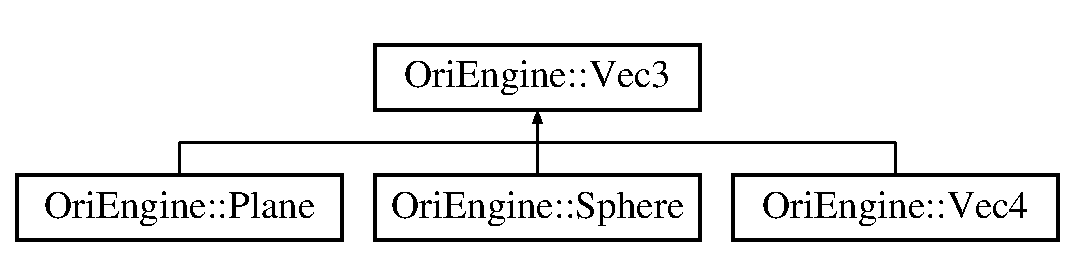
\includegraphics[height=2.000000cm]{struct_ori_engine_1_1_vec3}
\end{center}
\end{figure}
\subsection*{Public Member Functions}
\begin{DoxyCompactItemize}
\item 
void \hyperlink{struct_ori_engine_1_1_vec3_a5b144d090843acf90840393a1099a228}{Load} (float \+\_\+x, float \+\_\+y, float \+\_\+z)
\begin{DoxyCompactList}\small\item\em Structures are default public! \end{DoxyCompactList}\item 
\hyperlink{struct_ori_engine_1_1_vec3_a36bb2140a6a15310e08b4daaaf9a3909}{Vec3} (float s=float(0.\+0))
\begin{DoxyCompactList}\small\item\em Here\textquotesingle{}s a set of constructors. \end{DoxyCompactList}\item 
\hyperlink{struct_ori_engine_1_1_vec3_af2c77725c493c84a934fb358b311d87e}{Vec3} (float \+\_\+x, float \+\_\+y, float \+\_\+z)
\item 
\hyperlink{struct_ori_engine_1_1_vec3_adb231ac012b0ca1101b7e340bf2a72b0}{Vec3} (const \hyperlink{struct_ori_engine_1_1_vec3}{Vec3} \&v)
\begin{DoxyCompactList}\small\item\em A copy constructor. \end{DoxyCompactList}\item 
\hyperlink{struct_ori_engine_1_1_vec3}{Vec3} \& \hyperlink{struct_ori_engine_1_1_vec3_ab162ac7e06cb783bccc3375f9c75308a}{operator=} (const \hyperlink{struct_ori_engine_1_1_vec3}{Vec3} \&v)
\begin{DoxyCompactList}\small\item\em Operator overloads (see note 1 at the end of this file) \end{DoxyCompactList}\item 
const float \hyperlink{struct_ori_engine_1_1_vec3_a536dde0bfab3d42f2bae717b3b58df62}{operator\mbox{[}$\,$\mbox{]}} (int index) const
\begin{DoxyCompactList}\small\item\em Now we can use the \hyperlink{struct_ori_engine_1_1_vec3}{Vec3} like an array but we\textquotesingle{}ll need two overloads. \end{DoxyCompactList}\item 
float \& \hyperlink{struct_ori_engine_1_1_vec3_a71c0ae39cb5f864517078494ea528970}{operator\mbox{[}$\,$\mbox{]}} (int index)
\item 
const \hyperlink{struct_ori_engine_1_1_vec3}{Vec3} \hyperlink{struct_ori_engine_1_1_vec3_a68b3819fa6b6b9ddb2d6c1d75caa0d41}{operator+} (const \hyperlink{struct_ori_engine_1_1_vec3}{Vec3} \&v) const
\begin{DoxyCompactList}\small\item\em Add two Vec3s. \end{DoxyCompactList}\item 
\hyperlink{struct_ori_engine_1_1_vec3}{Vec3} \& \hyperlink{struct_ori_engine_1_1_vec3_a1f77d29a453dfdf1fc75290e2824b42e}{operator+=} (const \hyperlink{struct_ori_engine_1_1_vec3}{Vec3} \&v)
\begin{DoxyCompactList}\small\item\em Add a \hyperlink{struct_ori_engine_1_1_vec3}{Vec3} to itself. \end{DoxyCompactList}\item 
const \hyperlink{struct_ori_engine_1_1_vec3}{Vec3} \hyperlink{struct_ori_engine_1_1_vec3_a15bce489607090ec4bda56a1d5b0c0f1}{operator-\/} () const
\begin{DoxyCompactList}\small\item\em Take the negative of a \hyperlink{struct_ori_engine_1_1_vec3}{Vec3}. \end{DoxyCompactList}\item 
const \hyperlink{struct_ori_engine_1_1_vec3}{Vec3} \hyperlink{struct_ori_engine_1_1_vec3_a18dacfa9dfb456dd11e58a7be4f01e8d}{operator-\/} (const \hyperlink{struct_ori_engine_1_1_vec3}{Vec3} \&v) const
\begin{DoxyCompactList}\small\item\em Subtract two Vec3s. \end{DoxyCompactList}\item 
\hyperlink{struct_ori_engine_1_1_vec3}{Vec3} \& \hyperlink{struct_ori_engine_1_1_vec3_a5ced07421d0576122c0179517947039b}{operator-\/=} (const \hyperlink{struct_ori_engine_1_1_vec3}{Vec3} \&v)
\begin{DoxyCompactList}\small\item\em Subtract a Vec 3 from itself. \end{DoxyCompactList}\item 
const \hyperlink{struct_ori_engine_1_1_vec3}{Vec3} \hyperlink{struct_ori_engine_1_1_vec3_ac32d680353a0bdf43f6ab113834e1986}{operator$\ast$} (const float s) const
\begin{DoxyCompactList}\small\item\em Multiply a \hyperlink{struct_ori_engine_1_1_vec3}{Vec3} by a scalar. \end{DoxyCompactList}\item 
\hyperlink{struct_ori_engine_1_1_vec3}{Vec3} \& \hyperlink{struct_ori_engine_1_1_vec3_a93473080cc10ee1c3554a9557d467215}{operator$\ast$=} (const float s)
\begin{DoxyCompactList}\small\item\em Multiply a \hyperlink{struct_ori_engine_1_1_vec3}{Vec3} by a scalar and assign it to itself. \end{DoxyCompactList}\item 
const \hyperlink{struct_ori_engine_1_1_vec3}{Vec3} \hyperlink{struct_ori_engine_1_1_vec3_ae3a5cf75e250a543b1045be44b954950}{operator/} (const float s) const
\begin{DoxyCompactList}\small\item\em Divide by a scalar -\/ Watch for divide by zero issues. \end{DoxyCompactList}\item 
\hyperlink{struct_ori_engine_1_1_vec3}{Vec3} \& \hyperlink{struct_ori_engine_1_1_vec3_a8931b41bd47e616624c49320bd83e959}{operator/=} (const float s)
\item 
void \hyperlink{struct_ori_engine_1_1_vec3_a87155de383da7584fbe0725b3a4e371d}{print} ()
\end{DoxyCompactItemize}
\subsection*{Public Attributes}
\begin{DoxyCompactItemize}
\item 
float \hyperlink{struct_ori_engine_1_1_vec3_a2682de13a3ac0391777172f7f0af4027}{x}
\item 
float \hyperlink{struct_ori_engine_1_1_vec3_af7815329fe7e5d909afea88c87ac9ff6}{y}
\item 
float \hyperlink{struct_ori_engine_1_1_vec3_a9d4a41bdb6ce600fa8a23d27752ba2d1}{z}
\end{DoxyCompactItemize}
\subsection*{Friends}
\begin{DoxyCompactItemize}
\item 
\hyperlink{struct_ori_engine_1_1_vec3}{Vec3} \hyperlink{struct_ori_engine_1_1_vec3_aadc3cbbff02e566f5b84a5cccc5e0fa0}{operator$\ast$} (const float s, const \hyperlink{struct_ori_engine_1_1_vec3}{Vec3} \&v)
\end{DoxyCompactItemize}


\subsection{Constructor \& Destructor Documentation}
\hypertarget{struct_ori_engine_1_1_vec3_a36bb2140a6a15310e08b4daaaf9a3909}{}\label{struct_ori_engine_1_1_vec3_a36bb2140a6a15310e08b4daaaf9a3909} 
\index{Ori\+Engine\+::\+Vec3@{Ori\+Engine\+::\+Vec3}!Vec3@{Vec3}}
\index{Vec3@{Vec3}!Ori\+Engine\+::\+Vec3@{Ori\+Engine\+::\+Vec3}}
\subsubsection{\texorpdfstring{Vec3()}{Vec3()}\hspace{0.1cm}{\footnotesize\ttfamily [1/3]}}
{\footnotesize\ttfamily Ori\+Engine\+::\+Vec3\+::\+Vec3 (\begin{DoxyParamCaption}\item[{float}]{s = {\ttfamily float(0.0)} }\end{DoxyParamCaption})\hspace{0.3cm}{\ttfamily [inline]}}



Here\textquotesingle{}s a set of constructors. 

\hypertarget{struct_ori_engine_1_1_vec3_af2c77725c493c84a934fb358b311d87e}{}\label{struct_ori_engine_1_1_vec3_af2c77725c493c84a934fb358b311d87e} 
\index{Ori\+Engine\+::\+Vec3@{Ori\+Engine\+::\+Vec3}!Vec3@{Vec3}}
\index{Vec3@{Vec3}!Ori\+Engine\+::\+Vec3@{Ori\+Engine\+::\+Vec3}}
\subsubsection{\texorpdfstring{Vec3()}{Vec3()}\hspace{0.1cm}{\footnotesize\ttfamily [2/3]}}
{\footnotesize\ttfamily Ori\+Engine\+::\+Vec3\+::\+Vec3 (\begin{DoxyParamCaption}\item[{float}]{\+\_\+x,  }\item[{float}]{\+\_\+y,  }\item[{float}]{\+\_\+z }\end{DoxyParamCaption})\hspace{0.3cm}{\ttfamily [inline]}}

\hypertarget{struct_ori_engine_1_1_vec3_adb231ac012b0ca1101b7e340bf2a72b0}{}\label{struct_ori_engine_1_1_vec3_adb231ac012b0ca1101b7e340bf2a72b0} 
\index{Ori\+Engine\+::\+Vec3@{Ori\+Engine\+::\+Vec3}!Vec3@{Vec3}}
\index{Vec3@{Vec3}!Ori\+Engine\+::\+Vec3@{Ori\+Engine\+::\+Vec3}}
\subsubsection{\texorpdfstring{Vec3()}{Vec3()}\hspace{0.1cm}{\footnotesize\ttfamily [3/3]}}
{\footnotesize\ttfamily Ori\+Engine\+::\+Vec3\+::\+Vec3 (\begin{DoxyParamCaption}\item[{const \hyperlink{struct_ori_engine_1_1_vec3}{Vec3} \&}]{v }\end{DoxyParamCaption})\hspace{0.3cm}{\ttfamily [inline]}}



A copy constructor. 

In this context \char`\"{}const\char`\"{} means I promise not to modify anything v points to 

\subsection{Member Function Documentation}
\hypertarget{struct_ori_engine_1_1_vec3_a5b144d090843acf90840393a1099a228}{}\label{struct_ori_engine_1_1_vec3_a5b144d090843acf90840393a1099a228} 
\index{Ori\+Engine\+::\+Vec3@{Ori\+Engine\+::\+Vec3}!Load@{Load}}
\index{Load@{Load}!Ori\+Engine\+::\+Vec3@{Ori\+Engine\+::\+Vec3}}
\subsubsection{\texorpdfstring{Load()}{Load()}}
{\footnotesize\ttfamily void Ori\+Engine\+::\+Vec3\+::\+Load (\begin{DoxyParamCaption}\item[{float}]{\+\_\+x,  }\item[{float}]{\+\_\+y,  }\item[{float}]{\+\_\+z }\end{DoxyParamCaption})\hspace{0.3cm}{\ttfamily [inline]}}



Structures are default public! 

Just a little utility to populate a vector \hypertarget{struct_ori_engine_1_1_vec3_ac32d680353a0bdf43f6ab113834e1986}{}\label{struct_ori_engine_1_1_vec3_ac32d680353a0bdf43f6ab113834e1986} 
\index{Ori\+Engine\+::\+Vec3@{Ori\+Engine\+::\+Vec3}!operator$\ast$@{operator$\ast$}}
\index{operator$\ast$@{operator$\ast$}!Ori\+Engine\+::\+Vec3@{Ori\+Engine\+::\+Vec3}}
\subsubsection{\texorpdfstring{operator$\ast$()}{operator*()}}
{\footnotesize\ttfamily const \hyperlink{struct_ori_engine_1_1_vec3}{Vec3} Ori\+Engine\+::\+Vec3\+::operator$\ast$ (\begin{DoxyParamCaption}\item[{const float}]{s }\end{DoxyParamCaption}) const\hspace{0.3cm}{\ttfamily [inline]}}



Multiply a \hyperlink{struct_ori_engine_1_1_vec3}{Vec3} by a scalar. 

\hypertarget{struct_ori_engine_1_1_vec3_a93473080cc10ee1c3554a9557d467215}{}\label{struct_ori_engine_1_1_vec3_a93473080cc10ee1c3554a9557d467215} 
\index{Ori\+Engine\+::\+Vec3@{Ori\+Engine\+::\+Vec3}!operator$\ast$=@{operator$\ast$=}}
\index{operator$\ast$=@{operator$\ast$=}!Ori\+Engine\+::\+Vec3@{Ori\+Engine\+::\+Vec3}}
\subsubsection{\texorpdfstring{operator$\ast$=()}{operator*=()}}
{\footnotesize\ttfamily \hyperlink{struct_ori_engine_1_1_vec3}{Vec3}\& Ori\+Engine\+::\+Vec3\+::operator$\ast$= (\begin{DoxyParamCaption}\item[{const float}]{s }\end{DoxyParamCaption})\hspace{0.3cm}{\ttfamily [inline]}}



Multiply a \hyperlink{struct_ori_engine_1_1_vec3}{Vec3} by a scalar and assign it to itself. 

\hypertarget{struct_ori_engine_1_1_vec3_a68b3819fa6b6b9ddb2d6c1d75caa0d41}{}\label{struct_ori_engine_1_1_vec3_a68b3819fa6b6b9ddb2d6c1d75caa0d41} 
\index{Ori\+Engine\+::\+Vec3@{Ori\+Engine\+::\+Vec3}!operator+@{operator+}}
\index{operator+@{operator+}!Ori\+Engine\+::\+Vec3@{Ori\+Engine\+::\+Vec3}}
\subsubsection{\texorpdfstring{operator+()}{operator+()}}
{\footnotesize\ttfamily const \hyperlink{struct_ori_engine_1_1_vec3}{Vec3} Ori\+Engine\+::\+Vec3\+::operator+ (\begin{DoxyParamCaption}\item[{const \hyperlink{struct_ori_engine_1_1_vec3}{Vec3} \&}]{v }\end{DoxyParamCaption}) const\hspace{0.3cm}{\ttfamily [inline]}}



Add two Vec3s. 

\hypertarget{struct_ori_engine_1_1_vec3_a1f77d29a453dfdf1fc75290e2824b42e}{}\label{struct_ori_engine_1_1_vec3_a1f77d29a453dfdf1fc75290e2824b42e} 
\index{Ori\+Engine\+::\+Vec3@{Ori\+Engine\+::\+Vec3}!operator+=@{operator+=}}
\index{operator+=@{operator+=}!Ori\+Engine\+::\+Vec3@{Ori\+Engine\+::\+Vec3}}
\subsubsection{\texorpdfstring{operator+=()}{operator+=()}}
{\footnotesize\ttfamily \hyperlink{struct_ori_engine_1_1_vec3}{Vec3}\& Ori\+Engine\+::\+Vec3\+::operator+= (\begin{DoxyParamCaption}\item[{const \hyperlink{struct_ori_engine_1_1_vec3}{Vec3} \&}]{v }\end{DoxyParamCaption})\hspace{0.3cm}{\ttfamily [inline]}}



Add a \hyperlink{struct_ori_engine_1_1_vec3}{Vec3} to itself. 

\hypertarget{struct_ori_engine_1_1_vec3_a15bce489607090ec4bda56a1d5b0c0f1}{}\label{struct_ori_engine_1_1_vec3_a15bce489607090ec4bda56a1d5b0c0f1} 
\index{Ori\+Engine\+::\+Vec3@{Ori\+Engine\+::\+Vec3}!operator-\/@{operator-\/}}
\index{operator-\/@{operator-\/}!Ori\+Engine\+::\+Vec3@{Ori\+Engine\+::\+Vec3}}
\subsubsection{\texorpdfstring{operator-\/()}{operator-()}\hspace{0.1cm}{\footnotesize\ttfamily [1/2]}}
{\footnotesize\ttfamily const \hyperlink{struct_ori_engine_1_1_vec3}{Vec3} Ori\+Engine\+::\+Vec3\+::operator-\/ (\begin{DoxyParamCaption}{ }\end{DoxyParamCaption}) const\hspace{0.3cm}{\ttfamily [inline]}}



Take the negative of a \hyperlink{struct_ori_engine_1_1_vec3}{Vec3}. 

\hypertarget{struct_ori_engine_1_1_vec3_a18dacfa9dfb456dd11e58a7be4f01e8d}{}\label{struct_ori_engine_1_1_vec3_a18dacfa9dfb456dd11e58a7be4f01e8d} 
\index{Ori\+Engine\+::\+Vec3@{Ori\+Engine\+::\+Vec3}!operator-\/@{operator-\/}}
\index{operator-\/@{operator-\/}!Ori\+Engine\+::\+Vec3@{Ori\+Engine\+::\+Vec3}}
\subsubsection{\texorpdfstring{operator-\/()}{operator-()}\hspace{0.1cm}{\footnotesize\ttfamily [2/2]}}
{\footnotesize\ttfamily const \hyperlink{struct_ori_engine_1_1_vec3}{Vec3} Ori\+Engine\+::\+Vec3\+::operator-\/ (\begin{DoxyParamCaption}\item[{const \hyperlink{struct_ori_engine_1_1_vec3}{Vec3} \&}]{v }\end{DoxyParamCaption}) const\hspace{0.3cm}{\ttfamily [inline]}}



Subtract two Vec3s. 

\hypertarget{struct_ori_engine_1_1_vec3_a5ced07421d0576122c0179517947039b}{}\label{struct_ori_engine_1_1_vec3_a5ced07421d0576122c0179517947039b} 
\index{Ori\+Engine\+::\+Vec3@{Ori\+Engine\+::\+Vec3}!operator-\/=@{operator-\/=}}
\index{operator-\/=@{operator-\/=}!Ori\+Engine\+::\+Vec3@{Ori\+Engine\+::\+Vec3}}
\subsubsection{\texorpdfstring{operator-\/=()}{operator-=()}}
{\footnotesize\ttfamily \hyperlink{struct_ori_engine_1_1_vec3}{Vec3}\& Ori\+Engine\+::\+Vec3\+::operator-\/= (\begin{DoxyParamCaption}\item[{const \hyperlink{struct_ori_engine_1_1_vec3}{Vec3} \&}]{v }\end{DoxyParamCaption})\hspace{0.3cm}{\ttfamily [inline]}}



Subtract a Vec 3 from itself. 

\hypertarget{struct_ori_engine_1_1_vec3_ae3a5cf75e250a543b1045be44b954950}{}\label{struct_ori_engine_1_1_vec3_ae3a5cf75e250a543b1045be44b954950} 
\index{Ori\+Engine\+::\+Vec3@{Ori\+Engine\+::\+Vec3}!operator/@{operator/}}
\index{operator/@{operator/}!Ori\+Engine\+::\+Vec3@{Ori\+Engine\+::\+Vec3}}
\subsubsection{\texorpdfstring{operator/()}{operator/()}}
{\footnotesize\ttfamily const \hyperlink{struct_ori_engine_1_1_vec3}{Vec3} Ori\+Engine\+::\+Vec3\+::operator/ (\begin{DoxyParamCaption}\item[{const float}]{s }\end{DoxyParamCaption}) const\hspace{0.3cm}{\ttfamily [inline]}}



Divide by a scalar -\/ Watch for divide by zero issues. 

If in debug mode let\textquotesingle{}s worry about divide by zero or nearly zero!!! \hypertarget{struct_ori_engine_1_1_vec3_a8931b41bd47e616624c49320bd83e959}{}\label{struct_ori_engine_1_1_vec3_a8931b41bd47e616624c49320bd83e959} 
\index{Ori\+Engine\+::\+Vec3@{Ori\+Engine\+::\+Vec3}!operator/=@{operator/=}}
\index{operator/=@{operator/=}!Ori\+Engine\+::\+Vec3@{Ori\+Engine\+::\+Vec3}}
\subsubsection{\texorpdfstring{operator/=()}{operator/=()}}
{\footnotesize\ttfamily \hyperlink{struct_ori_engine_1_1_vec3}{Vec3}\& Ori\+Engine\+::\+Vec3\+::operator/= (\begin{DoxyParamCaption}\item[{const float}]{s }\end{DoxyParamCaption})\hspace{0.3cm}{\ttfamily [inline]}}

If in debug mode let\textquotesingle{}s worry about divide by zero or nearly zero!!! \hypertarget{struct_ori_engine_1_1_vec3_ab162ac7e06cb783bccc3375f9c75308a}{}\label{struct_ori_engine_1_1_vec3_ab162ac7e06cb783bccc3375f9c75308a} 
\index{Ori\+Engine\+::\+Vec3@{Ori\+Engine\+::\+Vec3}!operator=@{operator=}}
\index{operator=@{operator=}!Ori\+Engine\+::\+Vec3@{Ori\+Engine\+::\+Vec3}}
\subsubsection{\texorpdfstring{operator=()}{operator=()}}
{\footnotesize\ttfamily \hyperlink{struct_ori_engine_1_1_vec3}{Vec3}\& Ori\+Engine\+::\+Vec3\+::operator= (\begin{DoxyParamCaption}\item[{const \hyperlink{struct_ori_engine_1_1_vec3}{Vec3} \&}]{v }\end{DoxyParamCaption})\hspace{0.3cm}{\ttfamily [inline]}}



Operator overloads (see note 1 at the end of this file) 

An assignment operator \hypertarget{struct_ori_engine_1_1_vec3_a536dde0bfab3d42f2bae717b3b58df62}{}\label{struct_ori_engine_1_1_vec3_a536dde0bfab3d42f2bae717b3b58df62} 
\index{Ori\+Engine\+::\+Vec3@{Ori\+Engine\+::\+Vec3}!operator\mbox{[}\mbox{]}@{operator[]}}
\index{operator\mbox{[}\mbox{]}@{operator[]}!Ori\+Engine\+::\+Vec3@{Ori\+Engine\+::\+Vec3}}
\subsubsection{\texorpdfstring{operator[]()}{operator[]()}\hspace{0.1cm}{\footnotesize\ttfamily [1/2]}}
{\footnotesize\ttfamily const float Ori\+Engine\+::\+Vec3\+::operator\mbox{[}$\,$\mbox{]} (\begin{DoxyParamCaption}\item[{int}]{index }\end{DoxyParamCaption}) const\hspace{0.3cm}{\ttfamily [inline]}}



Now we can use the \hyperlink{struct_ori_engine_1_1_vec3}{Vec3} like an array but we\textquotesingle{}ll need two overloads. 

This one is for reading the \hyperlink{struct_ori_engine_1_1_vec3}{Vec3} as if where an array \hypertarget{struct_ori_engine_1_1_vec3_a71c0ae39cb5f864517078494ea528970}{}\label{struct_ori_engine_1_1_vec3_a71c0ae39cb5f864517078494ea528970} 
\index{Ori\+Engine\+::\+Vec3@{Ori\+Engine\+::\+Vec3}!operator\mbox{[}\mbox{]}@{operator[]}}
\index{operator\mbox{[}\mbox{]}@{operator[]}!Ori\+Engine\+::\+Vec3@{Ori\+Engine\+::\+Vec3}}
\subsubsection{\texorpdfstring{operator[]()}{operator[]()}\hspace{0.1cm}{\footnotesize\ttfamily [2/2]}}
{\footnotesize\ttfamily float\& Ori\+Engine\+::\+Vec3\+::operator\mbox{[}$\,$\mbox{]} (\begin{DoxyParamCaption}\item[{int}]{index }\end{DoxyParamCaption})\hspace{0.3cm}{\ttfamily [inline]}}

This one is for writing to the \hyperlink{struct_ori_engine_1_1_vec3}{Vec3} as if where an array.

See note 2 at the end of this file about lvalues and rvalues \hypertarget{struct_ori_engine_1_1_vec3_a87155de383da7584fbe0725b3a4e371d}{}\label{struct_ori_engine_1_1_vec3_a87155de383da7584fbe0725b3a4e371d} 
\index{Ori\+Engine\+::\+Vec3@{Ori\+Engine\+::\+Vec3}!print@{print}}
\index{print@{print}!Ori\+Engine\+::\+Vec3@{Ori\+Engine\+::\+Vec3}}
\subsubsection{\texorpdfstring{print()}{print()}}
{\footnotesize\ttfamily void Ori\+Engine\+::\+Vec3\+::print (\begin{DoxyParamCaption}{ }\end{DoxyParamCaption})\hspace{0.3cm}{\ttfamily [inline]}}



\subsection{Friends And Related Function Documentation}
\hypertarget{struct_ori_engine_1_1_vec3_aadc3cbbff02e566f5b84a5cccc5e0fa0}{}\label{struct_ori_engine_1_1_vec3_aadc3cbbff02e566f5b84a5cccc5e0fa0} 
\index{Ori\+Engine\+::\+Vec3@{Ori\+Engine\+::\+Vec3}!operator$\ast$@{operator$\ast$}}
\index{operator$\ast$@{operator$\ast$}!Ori\+Engine\+::\+Vec3@{Ori\+Engine\+::\+Vec3}}
\subsubsection{\texorpdfstring{operator$\ast$}{operator*}}
{\footnotesize\ttfamily \hyperlink{struct_ori_engine_1_1_vec3}{Vec3} operator$\ast$ (\begin{DoxyParamCaption}\item[{const float}]{s,  }\item[{const \hyperlink{struct_ori_engine_1_1_vec3}{Vec3} \&}]{v }\end{DoxyParamCaption})\hspace{0.3cm}{\ttfamily [friend]}}

Multiply a scaler by a \hyperlink{struct_ori_engine_1_1_vec3}{Vec3} -\/ Ha! It\textquotesingle{}s the scalar first then the \hyperlink{struct_ori_engine_1_1_vec3}{Vec3} Overloaded and a friend, ouch! It\textquotesingle{}s the only way to make it work with a scalar first. Friends are tricky, look them up. 

\subsection{Member Data Documentation}
\hypertarget{struct_ori_engine_1_1_vec3_a2682de13a3ac0391777172f7f0af4027}{}\label{struct_ori_engine_1_1_vec3_a2682de13a3ac0391777172f7f0af4027} 
\index{Ori\+Engine\+::\+Vec3@{Ori\+Engine\+::\+Vec3}!x@{x}}
\index{x@{x}!Ori\+Engine\+::\+Vec3@{Ori\+Engine\+::\+Vec3}}
\subsubsection{\texorpdfstring{x}{x}}
{\footnotesize\ttfamily float Ori\+Engine\+::\+Vec3\+::x}

\hypertarget{struct_ori_engine_1_1_vec3_af7815329fe7e5d909afea88c87ac9ff6}{}\label{struct_ori_engine_1_1_vec3_af7815329fe7e5d909afea88c87ac9ff6} 
\index{Ori\+Engine\+::\+Vec3@{Ori\+Engine\+::\+Vec3}!y@{y}}
\index{y@{y}!Ori\+Engine\+::\+Vec3@{Ori\+Engine\+::\+Vec3}}
\subsubsection{\texorpdfstring{y}{y}}
{\footnotesize\ttfamily float Ori\+Engine\+::\+Vec3\+::y}

\hypertarget{struct_ori_engine_1_1_vec3_a9d4a41bdb6ce600fa8a23d27752ba2d1}{}\label{struct_ori_engine_1_1_vec3_a9d4a41bdb6ce600fa8a23d27752ba2d1} 
\index{Ori\+Engine\+::\+Vec3@{Ori\+Engine\+::\+Vec3}!z@{z}}
\index{z@{z}!Ori\+Engine\+::\+Vec3@{Ori\+Engine\+::\+Vec3}}
\subsubsection{\texorpdfstring{z}{z}}
{\footnotesize\ttfamily float Ori\+Engine\+::\+Vec3\+::z}



The documentation for this struct was generated from the following file\+:\begin{DoxyCompactItemize}
\item 
Ori\+Engine/\+Ori\+Engine/\hyperlink{_vector_8h}{Vector.\+h}\end{DoxyCompactItemize}

\hypertarget{struct_ori_engine_1_1_vec4}{}\section{Ori\+Engine\+:\+:Vec4 Struct Reference}
\label{struct_ori_engine_1_1_vec4}\index{Ori\+Engine\+::\+Vec4@{Ori\+Engine\+::\+Vec4}}


{\ttfamily \#include $<$Vector.\+h$>$}

Inheritance diagram for Ori\+Engine\+:\+:Vec4\+:\begin{figure}[H]
\begin{center}
\leavevmode
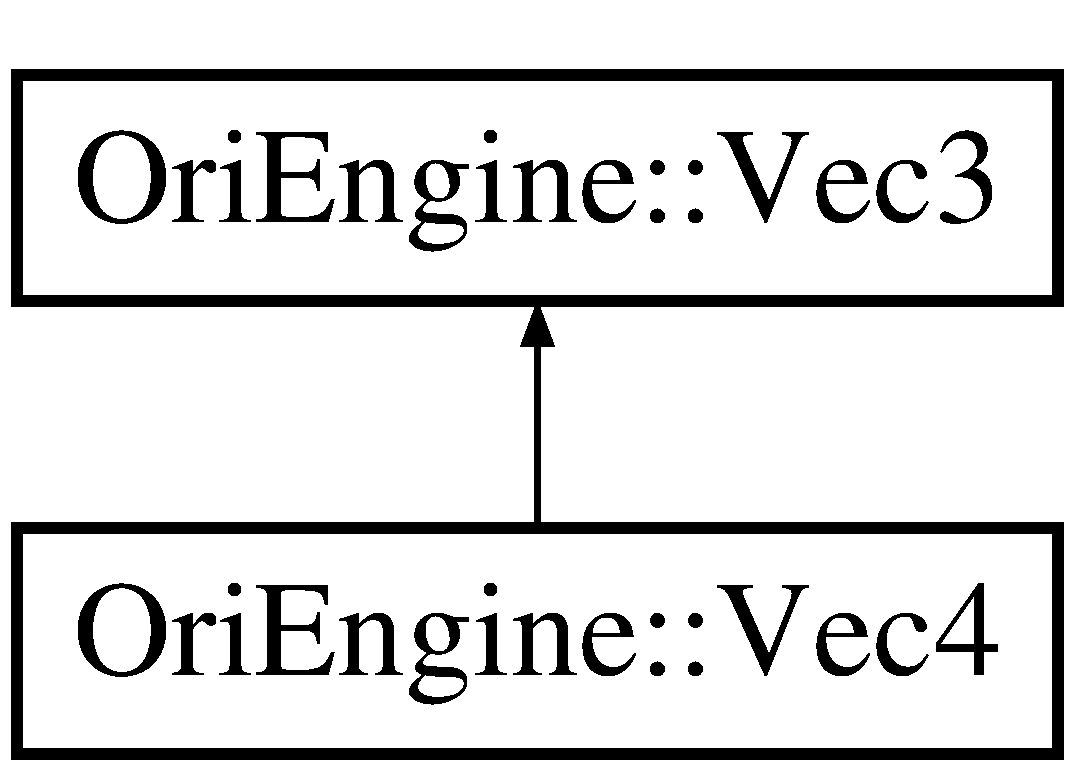
\includegraphics[height=2.000000cm]{struct_ori_engine_1_1_vec4}
\end{center}
\end{figure}
\subsection*{Public Member Functions}
\begin{DoxyCompactItemize}
\item 
\hyperlink{struct_ori_engine_1_1_vec4_a28be40c1d1f863b5d62ca6283c49e388}{Vec4} (float s=float(0.\+0))
\begin{DoxyCompactList}\small\item\em Here\textquotesingle{}s a set of constructors. \end{DoxyCompactList}\item 
\hyperlink{struct_ori_engine_1_1_vec4_af1620f14a897f7a9f94fbcd1e91fb9de}{Vec4} (float \+\_\+x, float \+\_\+y, float \+\_\+z, float \+\_\+w)
\item 
\hyperlink{struct_ori_engine_1_1_vec4_ae1591588e904abd9bd0772d81a50194f}{Vec4} (const \hyperlink{struct_ori_engine_1_1_vec4}{Vec4} \&v)
\item 
\hyperlink{struct_ori_engine_1_1_vec4_a703f1e094f1507602736d338bbe16f71}{Vec4} (const \hyperlink{struct_ori_engine_1_1_vec3}{Vec3} \&v)
\item 
\hyperlink{struct_ori_engine_1_1_vec4}{Vec4} \& \hyperlink{struct_ori_engine_1_1_vec4_a47afc3fac3c12536ef2fd980fb822ff6}{operator=} (const \hyperlink{struct_ori_engine_1_1_vec4}{Vec4} \&v)
\begin{DoxyCompactList}\small\item\em An assignment operator. \end{DoxyCompactList}\item 
float \& \hyperlink{struct_ori_engine_1_1_vec4_a8b078fddd99fc65f2a54a08948c56879}{operator\mbox{[}$\,$\mbox{]}} (int index)
\begin{DoxyCompactList}\small\item\em See \hyperlink{struct_ori_engine_1_1_vec3}{Vec3} definition. \end{DoxyCompactList}\item 
const float \hyperlink{struct_ori_engine_1_1_vec4_a5c5dea0b9eba3a118dbedf5ec57f3caf}{operator\mbox{[}$\,$\mbox{]}} (int i) const
\item 
\hyperlink{struct_ori_engine_1_1_vec4}{Vec4} \hyperlink{struct_ori_engine_1_1_vec4_a4d734f0ecb0ed6e41646ac9648dc0565}{operator+} (const \hyperlink{struct_ori_engine_1_1_vec4}{Vec4} \&v) const
\begin{DoxyCompactList}\small\item\em See \hyperlink{struct_ori_engine_1_1_vec3}{Vec3} definition. \end{DoxyCompactList}\item 
\hyperlink{struct_ori_engine_1_1_vec4}{Vec4} \& \hyperlink{struct_ori_engine_1_1_vec4_a49a96e495f80b4c03df2353ac88654a2}{operator+=} (const \hyperlink{struct_ori_engine_1_1_vec4}{Vec4} \&v)
\begin{DoxyCompactList}\small\item\em See \hyperlink{struct_ori_engine_1_1_vec3}{Vec3} definition. \end{DoxyCompactList}\item 
\hyperlink{struct_ori_engine_1_1_vec4}{Vec4} \hyperlink{struct_ori_engine_1_1_vec4_aa84e93dcbac56ffa66068af8abd1aed5}{operator-\/} () const
\item 
\hyperlink{struct_ori_engine_1_1_vec4}{Vec4} \hyperlink{struct_ori_engine_1_1_vec4_ab9f5420252322ccd1a683a78eb7177cb}{operator-\/} (const \hyperlink{struct_ori_engine_1_1_vec4}{Vec4} \&v) const
\begin{DoxyCompactList}\small\item\em See \hyperlink{struct_ori_engine_1_1_vec3}{Vec3} definition. \end{DoxyCompactList}\item 
\hyperlink{struct_ori_engine_1_1_vec4}{Vec4} \& \hyperlink{struct_ori_engine_1_1_vec4_a213cbae8de217866744a5c83349c4033}{operator-\/=} (const \hyperlink{struct_ori_engine_1_1_vec4}{Vec4} \&v)
\begin{DoxyCompactList}\small\item\em See \hyperlink{struct_ori_engine_1_1_vec3}{Vec3} definition. \end{DoxyCompactList}\item 
\hyperlink{struct_ori_engine_1_1_vec4}{Vec4} \hyperlink{struct_ori_engine_1_1_vec4_adbd1dee1fe6d1ebc4b9f72a66b8de0b6}{operator$\ast$} (const float s) const
\begin{DoxyCompactList}\small\item\em See \hyperlink{struct_ori_engine_1_1_vec3}{Vec3} definition. \end{DoxyCompactList}\item 
\hyperlink{struct_ori_engine_1_1_vec4}{Vec4} \& \hyperlink{struct_ori_engine_1_1_vec4_a104e6844bc375f3a88d8497bc65a4ec3}{operator$\ast$=} (const float s)
\begin{DoxyCompactList}\small\item\em See \hyperlink{struct_ori_engine_1_1_vec3}{Vec3} definition. \end{DoxyCompactList}\item 
\hyperlink{struct_ori_engine_1_1_vec4}{Vec4} \hyperlink{struct_ori_engine_1_1_vec4_aa6e144f7ab67f6dfcaf09a02067c5b57}{operator/} (const float s) const
\item 
\hyperlink{struct_ori_engine_1_1_vec4}{Vec4} \& \hyperlink{struct_ori_engine_1_1_vec4_af0fc00ff1ac696f44b2cc2addd9be4bb}{operator/=} (const float s)
\item 
void \hyperlink{struct_ori_engine_1_1_vec4_a3ed05625c5422292da6218fc6294c85c}{print} ()
\item 
\hyperlink{struct_ori_engine_1_1_vec4_a51a4a0aa30a09d5de4a38925d230c847}{operator const float $\ast$} () const
\item 
\hyperlink{struct_ori_engine_1_1_vec4_a9f1df44372c5cfb62e42741684bff87d}{operator float $\ast$} ()
\end{DoxyCompactItemize}
\subsection*{Public Attributes}
\begin{DoxyCompactItemize}
\item 
float \hyperlink{struct_ori_engine_1_1_vec4_ab69be65aad84be7c1904aef48cb34f95}{w}
\end{DoxyCompactItemize}
\subsection*{Friends}
\begin{DoxyCompactItemize}
\item 
\hyperlink{struct_ori_engine_1_1_vec4}{Vec4} \hyperlink{struct_ori_engine_1_1_vec4_a23071d3ed3480029acaf809bdaf37c24}{operator$\ast$} (const float s, const \hyperlink{struct_ori_engine_1_1_vec4}{Vec4} \&v)
\begin{DoxyCompactList}\small\item\em See \hyperlink{struct_ori_engine_1_1_vec3}{Vec3} definition. \end{DoxyCompactList}\end{DoxyCompactItemize}


\subsection{Detailed Description}
\hyperlink{struct_ori_engine_1_1_vec4}{Vec4} definitions I am intentionally creating a \hyperlink{struct_ori_engine_1_1_vec4}{Vec4} from a \hyperlink{struct_ori_engine_1_1_vec3}{Vec3} so I can pass a \hyperlink{struct_ori_engine_1_1_vec4}{Vec4} into a Subroutine that wants a \hyperlink{struct_ori_engine_1_1_vec3}{Vec3} in many cases this will be mathamatically OK, just be careful 

\subsection{Constructor \& Destructor Documentation}
\hypertarget{struct_ori_engine_1_1_vec4_a28be40c1d1f863b5d62ca6283c49e388}{}\label{struct_ori_engine_1_1_vec4_a28be40c1d1f863b5d62ca6283c49e388} 
\index{Ori\+Engine\+::\+Vec4@{Ori\+Engine\+::\+Vec4}!Vec4@{Vec4}}
\index{Vec4@{Vec4}!Ori\+Engine\+::\+Vec4@{Ori\+Engine\+::\+Vec4}}
\subsubsection{\texorpdfstring{Vec4()}{Vec4()}\hspace{0.1cm}{\footnotesize\ttfamily [1/4]}}
{\footnotesize\ttfamily Ori\+Engine\+::\+Vec4\+::\+Vec4 (\begin{DoxyParamCaption}\item[{float}]{s = {\ttfamily float(0.0)} }\end{DoxyParamCaption})\hspace{0.3cm}{\ttfamily [inline]}}



Here\textquotesingle{}s a set of constructors. 

\hypertarget{struct_ori_engine_1_1_vec4_af1620f14a897f7a9f94fbcd1e91fb9de}{}\label{struct_ori_engine_1_1_vec4_af1620f14a897f7a9f94fbcd1e91fb9de} 
\index{Ori\+Engine\+::\+Vec4@{Ori\+Engine\+::\+Vec4}!Vec4@{Vec4}}
\index{Vec4@{Vec4}!Ori\+Engine\+::\+Vec4@{Ori\+Engine\+::\+Vec4}}
\subsubsection{\texorpdfstring{Vec4()}{Vec4()}\hspace{0.1cm}{\footnotesize\ttfamily [2/4]}}
{\footnotesize\ttfamily Ori\+Engine\+::\+Vec4\+::\+Vec4 (\begin{DoxyParamCaption}\item[{float}]{\+\_\+x,  }\item[{float}]{\+\_\+y,  }\item[{float}]{\+\_\+z,  }\item[{float}]{\+\_\+w }\end{DoxyParamCaption})\hspace{0.3cm}{\ttfamily [inline]}}

\hypertarget{struct_ori_engine_1_1_vec4_ae1591588e904abd9bd0772d81a50194f}{}\label{struct_ori_engine_1_1_vec4_ae1591588e904abd9bd0772d81a50194f} 
\index{Ori\+Engine\+::\+Vec4@{Ori\+Engine\+::\+Vec4}!Vec4@{Vec4}}
\index{Vec4@{Vec4}!Ori\+Engine\+::\+Vec4@{Ori\+Engine\+::\+Vec4}}
\subsubsection{\texorpdfstring{Vec4()}{Vec4()}\hspace{0.1cm}{\footnotesize\ttfamily [3/4]}}
{\footnotesize\ttfamily Ori\+Engine\+::\+Vec4\+::\+Vec4 (\begin{DoxyParamCaption}\item[{const \hyperlink{struct_ori_engine_1_1_vec4}{Vec4} \&}]{v }\end{DoxyParamCaption})\hspace{0.3cm}{\ttfamily [inline]}}

\hypertarget{struct_ori_engine_1_1_vec4_a703f1e094f1507602736d338bbe16f71}{}\label{struct_ori_engine_1_1_vec4_a703f1e094f1507602736d338bbe16f71} 
\index{Ori\+Engine\+::\+Vec4@{Ori\+Engine\+::\+Vec4}!Vec4@{Vec4}}
\index{Vec4@{Vec4}!Ori\+Engine\+::\+Vec4@{Ori\+Engine\+::\+Vec4}}
\subsubsection{\texorpdfstring{Vec4()}{Vec4()}\hspace{0.1cm}{\footnotesize\ttfamily [4/4]}}
{\footnotesize\ttfamily Ori\+Engine\+::\+Vec4\+::\+Vec4 (\begin{DoxyParamCaption}\item[{const \hyperlink{struct_ori_engine_1_1_vec3}{Vec3} \&}]{v }\end{DoxyParamCaption})\hspace{0.3cm}{\ttfamily [inline]}}



\subsection{Member Function Documentation}
\hypertarget{struct_ori_engine_1_1_vec4_a51a4a0aa30a09d5de4a38925d230c847}{}\label{struct_ori_engine_1_1_vec4_a51a4a0aa30a09d5de4a38925d230c847} 
\index{Ori\+Engine\+::\+Vec4@{Ori\+Engine\+::\+Vec4}!operator const float $\ast$@{operator const float $\ast$}}
\index{operator const float $\ast$@{operator const float $\ast$}!Ori\+Engine\+::\+Vec4@{Ori\+Engine\+::\+Vec4}}
\subsubsection{\texorpdfstring{operator const float $\ast$()}{operator const float *()}}
{\footnotesize\ttfamily Ori\+Engine\+::\+Vec4\+::operator const float $\ast$ (\begin{DoxyParamCaption}{ }\end{DoxyParamCaption}) const\hspace{0.3cm}{\ttfamily [inline]}}

Type conversion operators \hypertarget{struct_ori_engine_1_1_vec4_a9f1df44372c5cfb62e42741684bff87d}{}\label{struct_ori_engine_1_1_vec4_a9f1df44372c5cfb62e42741684bff87d} 
\index{Ori\+Engine\+::\+Vec4@{Ori\+Engine\+::\+Vec4}!operator float $\ast$@{operator float $\ast$}}
\index{operator float $\ast$@{operator float $\ast$}!Ori\+Engine\+::\+Vec4@{Ori\+Engine\+::\+Vec4}}
\subsubsection{\texorpdfstring{operator float $\ast$()}{operator float *()}}
{\footnotesize\ttfamily Ori\+Engine\+::\+Vec4\+::operator float $\ast$ (\begin{DoxyParamCaption}{ }\end{DoxyParamCaption})\hspace{0.3cm}{\ttfamily [inline]}}

\hypertarget{struct_ori_engine_1_1_vec4_adbd1dee1fe6d1ebc4b9f72a66b8de0b6}{}\label{struct_ori_engine_1_1_vec4_adbd1dee1fe6d1ebc4b9f72a66b8de0b6} 
\index{Ori\+Engine\+::\+Vec4@{Ori\+Engine\+::\+Vec4}!operator$\ast$@{operator$\ast$}}
\index{operator$\ast$@{operator$\ast$}!Ori\+Engine\+::\+Vec4@{Ori\+Engine\+::\+Vec4}}
\subsubsection{\texorpdfstring{operator$\ast$()}{operator*()}}
{\footnotesize\ttfamily \hyperlink{struct_ori_engine_1_1_vec4}{Vec4} Ori\+Engine\+::\+Vec4\+::operator$\ast$ (\begin{DoxyParamCaption}\item[{const float}]{s }\end{DoxyParamCaption}) const\hspace{0.3cm}{\ttfamily [inline]}}



See \hyperlink{struct_ori_engine_1_1_vec3}{Vec3} definition. 

\hypertarget{struct_ori_engine_1_1_vec4_a104e6844bc375f3a88d8497bc65a4ec3}{}\label{struct_ori_engine_1_1_vec4_a104e6844bc375f3a88d8497bc65a4ec3} 
\index{Ori\+Engine\+::\+Vec4@{Ori\+Engine\+::\+Vec4}!operator$\ast$=@{operator$\ast$=}}
\index{operator$\ast$=@{operator$\ast$=}!Ori\+Engine\+::\+Vec4@{Ori\+Engine\+::\+Vec4}}
\subsubsection{\texorpdfstring{operator$\ast$=()}{operator*=()}}
{\footnotesize\ttfamily \hyperlink{struct_ori_engine_1_1_vec4}{Vec4}\& Ori\+Engine\+::\+Vec4\+::operator$\ast$= (\begin{DoxyParamCaption}\item[{const float}]{s }\end{DoxyParamCaption})\hspace{0.3cm}{\ttfamily [inline]}}



See \hyperlink{struct_ori_engine_1_1_vec3}{Vec3} definition. 

\hypertarget{struct_ori_engine_1_1_vec4_a4d734f0ecb0ed6e41646ac9648dc0565}{}\label{struct_ori_engine_1_1_vec4_a4d734f0ecb0ed6e41646ac9648dc0565} 
\index{Ori\+Engine\+::\+Vec4@{Ori\+Engine\+::\+Vec4}!operator+@{operator+}}
\index{operator+@{operator+}!Ori\+Engine\+::\+Vec4@{Ori\+Engine\+::\+Vec4}}
\subsubsection{\texorpdfstring{operator+()}{operator+()}}
{\footnotesize\ttfamily \hyperlink{struct_ori_engine_1_1_vec4}{Vec4} Ori\+Engine\+::\+Vec4\+::operator+ (\begin{DoxyParamCaption}\item[{const \hyperlink{struct_ori_engine_1_1_vec4}{Vec4} \&}]{v }\end{DoxyParamCaption}) const\hspace{0.3cm}{\ttfamily [inline]}}



See \hyperlink{struct_ori_engine_1_1_vec3}{Vec3} definition. 

\hypertarget{struct_ori_engine_1_1_vec4_a49a96e495f80b4c03df2353ac88654a2}{}\label{struct_ori_engine_1_1_vec4_a49a96e495f80b4c03df2353ac88654a2} 
\index{Ori\+Engine\+::\+Vec4@{Ori\+Engine\+::\+Vec4}!operator+=@{operator+=}}
\index{operator+=@{operator+=}!Ori\+Engine\+::\+Vec4@{Ori\+Engine\+::\+Vec4}}
\subsubsection{\texorpdfstring{operator+=()}{operator+=()}}
{\footnotesize\ttfamily \hyperlink{struct_ori_engine_1_1_vec4}{Vec4}\& Ori\+Engine\+::\+Vec4\+::operator+= (\begin{DoxyParamCaption}\item[{const \hyperlink{struct_ori_engine_1_1_vec4}{Vec4} \&}]{v }\end{DoxyParamCaption})\hspace{0.3cm}{\ttfamily [inline]}}



See \hyperlink{struct_ori_engine_1_1_vec3}{Vec3} definition. 

\hypertarget{struct_ori_engine_1_1_vec4_aa84e93dcbac56ffa66068af8abd1aed5}{}\label{struct_ori_engine_1_1_vec4_aa84e93dcbac56ffa66068af8abd1aed5} 
\index{Ori\+Engine\+::\+Vec4@{Ori\+Engine\+::\+Vec4}!operator-\/@{operator-\/}}
\index{operator-\/@{operator-\/}!Ori\+Engine\+::\+Vec4@{Ori\+Engine\+::\+Vec4}}
\subsubsection{\texorpdfstring{operator-\/()}{operator-()}\hspace{0.1cm}{\footnotesize\ttfamily [1/2]}}
{\footnotesize\ttfamily \hyperlink{struct_ori_engine_1_1_vec4}{Vec4} Ori\+Engine\+::\+Vec4\+::operator-\/ (\begin{DoxyParamCaption}{ }\end{DoxyParamCaption}) const\hspace{0.3cm}{\ttfamily [inline]}}

\hypertarget{struct_ori_engine_1_1_vec4_ab9f5420252322ccd1a683a78eb7177cb}{}\label{struct_ori_engine_1_1_vec4_ab9f5420252322ccd1a683a78eb7177cb} 
\index{Ori\+Engine\+::\+Vec4@{Ori\+Engine\+::\+Vec4}!operator-\/@{operator-\/}}
\index{operator-\/@{operator-\/}!Ori\+Engine\+::\+Vec4@{Ori\+Engine\+::\+Vec4}}
\subsubsection{\texorpdfstring{operator-\/()}{operator-()}\hspace{0.1cm}{\footnotesize\ttfamily [2/2]}}
{\footnotesize\ttfamily \hyperlink{struct_ori_engine_1_1_vec4}{Vec4} Ori\+Engine\+::\+Vec4\+::operator-\/ (\begin{DoxyParamCaption}\item[{const \hyperlink{struct_ori_engine_1_1_vec4}{Vec4} \&}]{v }\end{DoxyParamCaption}) const\hspace{0.3cm}{\ttfamily [inline]}}



See \hyperlink{struct_ori_engine_1_1_vec3}{Vec3} definition. 

\hypertarget{struct_ori_engine_1_1_vec4_a213cbae8de217866744a5c83349c4033}{}\label{struct_ori_engine_1_1_vec4_a213cbae8de217866744a5c83349c4033} 
\index{Ori\+Engine\+::\+Vec4@{Ori\+Engine\+::\+Vec4}!operator-\/=@{operator-\/=}}
\index{operator-\/=@{operator-\/=}!Ori\+Engine\+::\+Vec4@{Ori\+Engine\+::\+Vec4}}
\subsubsection{\texorpdfstring{operator-\/=()}{operator-=()}}
{\footnotesize\ttfamily \hyperlink{struct_ori_engine_1_1_vec4}{Vec4}\& Ori\+Engine\+::\+Vec4\+::operator-\/= (\begin{DoxyParamCaption}\item[{const \hyperlink{struct_ori_engine_1_1_vec4}{Vec4} \&}]{v }\end{DoxyParamCaption})\hspace{0.3cm}{\ttfamily [inline]}}



See \hyperlink{struct_ori_engine_1_1_vec3}{Vec3} definition. 

\hypertarget{struct_ori_engine_1_1_vec4_aa6e144f7ab67f6dfcaf09a02067c5b57}{}\label{struct_ori_engine_1_1_vec4_aa6e144f7ab67f6dfcaf09a02067c5b57} 
\index{Ori\+Engine\+::\+Vec4@{Ori\+Engine\+::\+Vec4}!operator/@{operator/}}
\index{operator/@{operator/}!Ori\+Engine\+::\+Vec4@{Ori\+Engine\+::\+Vec4}}
\subsubsection{\texorpdfstring{operator/()}{operator/()}}
{\footnotesize\ttfamily \hyperlink{struct_ori_engine_1_1_vec4}{Vec4} Ori\+Engine\+::\+Vec4\+::operator/ (\begin{DoxyParamCaption}\item[{const float}]{s }\end{DoxyParamCaption}) const\hspace{0.3cm}{\ttfamily [inline]}}

If in debug mode let\textquotesingle{}s worry about divide by zero or nearly zero!!! \hypertarget{struct_ori_engine_1_1_vec4_af0fc00ff1ac696f44b2cc2addd9be4bb}{}\label{struct_ori_engine_1_1_vec4_af0fc00ff1ac696f44b2cc2addd9be4bb} 
\index{Ori\+Engine\+::\+Vec4@{Ori\+Engine\+::\+Vec4}!operator/=@{operator/=}}
\index{operator/=@{operator/=}!Ori\+Engine\+::\+Vec4@{Ori\+Engine\+::\+Vec4}}
\subsubsection{\texorpdfstring{operator/=()}{operator/=()}}
{\footnotesize\ttfamily \hyperlink{struct_ori_engine_1_1_vec4}{Vec4}\& Ori\+Engine\+::\+Vec4\+::operator/= (\begin{DoxyParamCaption}\item[{const float}]{s }\end{DoxyParamCaption})\hspace{0.3cm}{\ttfamily [inline]}}

If in debug mode let\textquotesingle{}s worry about divide by zero or nearly zero!!! \hypertarget{struct_ori_engine_1_1_vec4_a47afc3fac3c12536ef2fd980fb822ff6}{}\label{struct_ori_engine_1_1_vec4_a47afc3fac3c12536ef2fd980fb822ff6} 
\index{Ori\+Engine\+::\+Vec4@{Ori\+Engine\+::\+Vec4}!operator=@{operator=}}
\index{operator=@{operator=}!Ori\+Engine\+::\+Vec4@{Ori\+Engine\+::\+Vec4}}
\subsubsection{\texorpdfstring{operator=()}{operator=()}}
{\footnotesize\ttfamily \hyperlink{struct_ori_engine_1_1_vec4}{Vec4}\& Ori\+Engine\+::\+Vec4\+::operator= (\begin{DoxyParamCaption}\item[{const \hyperlink{struct_ori_engine_1_1_vec4}{Vec4} \&}]{v }\end{DoxyParamCaption})\hspace{0.3cm}{\ttfamily [inline]}}



An assignment operator. 

\hypertarget{struct_ori_engine_1_1_vec4_a8b078fddd99fc65f2a54a08948c56879}{}\label{struct_ori_engine_1_1_vec4_a8b078fddd99fc65f2a54a08948c56879} 
\index{Ori\+Engine\+::\+Vec4@{Ori\+Engine\+::\+Vec4}!operator\mbox{[}\mbox{]}@{operator[]}}
\index{operator\mbox{[}\mbox{]}@{operator[]}!Ori\+Engine\+::\+Vec4@{Ori\+Engine\+::\+Vec4}}
\subsubsection{\texorpdfstring{operator[]()}{operator[]()}\hspace{0.1cm}{\footnotesize\ttfamily [1/2]}}
{\footnotesize\ttfamily float\& Ori\+Engine\+::\+Vec4\+::operator\mbox{[}$\,$\mbox{]} (\begin{DoxyParamCaption}\item[{int}]{index }\end{DoxyParamCaption})\hspace{0.3cm}{\ttfamily [inline]}}



See \hyperlink{struct_ori_engine_1_1_vec3}{Vec3} definition. 

\hypertarget{struct_ori_engine_1_1_vec4_a5c5dea0b9eba3a118dbedf5ec57f3caf}{}\label{struct_ori_engine_1_1_vec4_a5c5dea0b9eba3a118dbedf5ec57f3caf} 
\index{Ori\+Engine\+::\+Vec4@{Ori\+Engine\+::\+Vec4}!operator\mbox{[}\mbox{]}@{operator[]}}
\index{operator\mbox{[}\mbox{]}@{operator[]}!Ori\+Engine\+::\+Vec4@{Ori\+Engine\+::\+Vec4}}
\subsubsection{\texorpdfstring{operator[]()}{operator[]()}\hspace{0.1cm}{\footnotesize\ttfamily [2/2]}}
{\footnotesize\ttfamily const float Ori\+Engine\+::\+Vec4\+::operator\mbox{[}$\,$\mbox{]} (\begin{DoxyParamCaption}\item[{int}]{i }\end{DoxyParamCaption}) const\hspace{0.3cm}{\ttfamily [inline]}}

\hypertarget{struct_ori_engine_1_1_vec4_a3ed05625c5422292da6218fc6294c85c}{}\label{struct_ori_engine_1_1_vec4_a3ed05625c5422292da6218fc6294c85c} 
\index{Ori\+Engine\+::\+Vec4@{Ori\+Engine\+::\+Vec4}!print@{print}}
\index{print@{print}!Ori\+Engine\+::\+Vec4@{Ori\+Engine\+::\+Vec4}}
\subsubsection{\texorpdfstring{print()}{print()}}
{\footnotesize\ttfamily void Ori\+Engine\+::\+Vec4\+::print (\begin{DoxyParamCaption}{ }\end{DoxyParamCaption})\hspace{0.3cm}{\ttfamily [inline]}}



\subsection{Friends And Related Function Documentation}
\hypertarget{struct_ori_engine_1_1_vec4_a23071d3ed3480029acaf809bdaf37c24}{}\label{struct_ori_engine_1_1_vec4_a23071d3ed3480029acaf809bdaf37c24} 
\index{Ori\+Engine\+::\+Vec4@{Ori\+Engine\+::\+Vec4}!operator$\ast$@{operator$\ast$}}
\index{operator$\ast$@{operator$\ast$}!Ori\+Engine\+::\+Vec4@{Ori\+Engine\+::\+Vec4}}
\subsubsection{\texorpdfstring{operator$\ast$}{operator*}}
{\footnotesize\ttfamily \hyperlink{struct_ori_engine_1_1_vec4}{Vec4} operator$\ast$ (\begin{DoxyParamCaption}\item[{const float}]{s,  }\item[{const \hyperlink{struct_ori_engine_1_1_vec4}{Vec4} \&}]{v }\end{DoxyParamCaption})\hspace{0.3cm}{\ttfamily [friend]}}



See \hyperlink{struct_ori_engine_1_1_vec3}{Vec3} definition. 



\subsection{Member Data Documentation}
\hypertarget{struct_ori_engine_1_1_vec4_ab69be65aad84be7c1904aef48cb34f95}{}\label{struct_ori_engine_1_1_vec4_ab69be65aad84be7c1904aef48cb34f95} 
\index{Ori\+Engine\+::\+Vec4@{Ori\+Engine\+::\+Vec4}!w@{w}}
\index{w@{w}!Ori\+Engine\+::\+Vec4@{Ori\+Engine\+::\+Vec4}}
\subsubsection{\texorpdfstring{w}{w}}
{\footnotesize\ttfamily float Ori\+Engine\+::\+Vec4\+::w}

float x; /// float y; /// From \hyperlink{struct_ori_engine_1_1_vec3}{Vec3} float z; /// 

The documentation for this struct was generated from the following file\+:\begin{DoxyCompactItemize}
\item 
Ori\+Engine/\+Ori\+Engine/\hyperlink{_vector_8h}{Vector.\+h}\end{DoxyCompactItemize}

\hypertarget{class_ori_engine_1_1_window}{}\section{Ori\+Engine\+:\+:Window Class Reference}
\label{class_ori_engine_1_1_window}\index{Ori\+Engine\+::\+Window@{Ori\+Engine\+::\+Window}}


{\ttfamily \#include $<$Window.\+h$>$}

\subsection*{Public Member Functions}
\begin{DoxyCompactItemize}
\item 
\hyperlink{class_ori_engine_1_1_window_a74e6087da23d3c24e9fac0245e5ec92c}{Window} ()
\item 
\hyperlink{class_ori_engine_1_1_window_a16f73e151437c63953a6396aa80b686f}{Window} (const \hyperlink{class_ori_engine_1_1_window}{Window} \&)=delete
\item 
\hyperlink{class_ori_engine_1_1_window_acda5b9ba9a89a8bd8df298c1cedb71a8}{Window} (\hyperlink{class_ori_engine_1_1_window}{Window} \&\&)=delete
\item 
\hyperlink{class_ori_engine_1_1_window}{Window} \& \hyperlink{class_ori_engine_1_1_window_aad30c448f70cb9f20641289765e23350}{operator=} (const \hyperlink{class_ori_engine_1_1_window}{Window} \&)=delete
\item 
\hyperlink{class_ori_engine_1_1_window}{Window} \& \hyperlink{class_ori_engine_1_1_window_a54a09c75fc36036859b93c276ca834fa}{operator=} (\hyperlink{class_ori_engine_1_1_window}{Window} \&\&)=delete
\item 
\hyperlink{class_ori_engine_1_1_window_a245d821e6016fa1f6970ccbbedd635f6}{$\sim$\+Window} ()
\item 
bool \hyperlink{class_ori_engine_1_1_window_a41cab6dae60380563b8bc593e87f0c87}{Initialize} ()
\item 
void \hyperlink{class_ori_engine_1_1_window_a89c434ec340b4594c6c8af3f0bf58c9b}{Shutdown} ()
\item 
void \hyperlink{class_ori_engine_1_1_window_a21db050c674219f29a985694739ff31e}{Set\+Window\+Size} (const int Width\+\_\+, const int Height\+\_\+)
\item 
void \hyperlink{class_ori_engine_1_1_window_a65149d93f9842363f53bdc3e07f459a6}{Toggle\+Full\+Screen} ()
\item 
S\+D\+L\+\_\+\+Window $\ast$ \hyperlink{class_ori_engine_1_1_window_acf146679abf09abf89941b1882fc92dc}{get\+Window} () const
\item 
S\+D\+L\+\_\+\+Rect \hyperlink{class_ori_engine_1_1_window_a53ff5d3c56b28604d41b676bfdbf5129}{get\+Rect} ()
\item 
int \hyperlink{class_ori_engine_1_1_window_a451bdfeab37afce97712f23f5c2492aa}{Get\+Width} () const
\item 
int \hyperlink{class_ori_engine_1_1_window_a2196b5ae099037272cc85b223e80bd6d}{Get\+Height} () const
\end{DoxyCompactItemize}
\subsection*{Private Member Functions}
\begin{DoxyCompactItemize}
\item 
void \hyperlink{class_ori_engine_1_1_window_a8e80d9499f2968b20492b517006cc1b3}{get\+G\+L\+Info} ()
\begin{DoxyCompactList}\small\item\em Debug info about the graphics card and version of Open\+GL installed. \end{DoxyCompactList}\end{DoxyCompactItemize}
\subsection*{Private Attributes}
\begin{DoxyCompactItemize}
\item 
S\+D\+L\+\_\+\+Window $\ast$ \hyperlink{class_ori_engine_1_1_window_ab89e66fc9f835484f073a7ac7c1ee546}{S\+D\+L\+Window}
\item 
S\+D\+L\+\_\+\+G\+L\+Context \hyperlink{class_ori_engine_1_1_window_a1e0582658a858b0cfa732c990a8573c0}{gl\+Context}
\item 
int \hyperlink{class_ori_engine_1_1_window_a3f618d387c7429ade0b51f3c76c1ebb6}{Width}
\item 
int \hyperlink{class_ori_engine_1_1_window_a2315cbe759b91f12618a81f47b1f4c32}{Height}
\item 
S\+D\+L\+\_\+\+Rect \hyperlink{class_ori_engine_1_1_window_a1e2e93b43d6b1ca022ad8393db7ac35f}{win\+Rect}
\item 
bool \hyperlink{class_ori_engine_1_1_window_a9a2f58afdd7d2cdd920f7c733b4b7dd6}{b\+Is\+Initialized}
\item 
bool \hyperlink{class_ori_engine_1_1_window_a31ccebb8ecb24ead816ae2559e1e36d2}{b\+Is\+Full\+Screen}
\end{DoxyCompactItemize}


\subsection{Constructor \& Destructor Documentation}
\hypertarget{class_ori_engine_1_1_window_a74e6087da23d3c24e9fac0245e5ec92c}{}\label{class_ori_engine_1_1_window_a74e6087da23d3c24e9fac0245e5ec92c} 
\index{Ori\+Engine\+::\+Window@{Ori\+Engine\+::\+Window}!Window@{Window}}
\index{Window@{Window}!Ori\+Engine\+::\+Window@{Ori\+Engine\+::\+Window}}
\subsubsection{\texorpdfstring{Window()}{Window()}\hspace{0.1cm}{\footnotesize\ttfamily [1/3]}}
{\footnotesize\ttfamily Window\+::\+Window (\begin{DoxyParamCaption}{ }\end{DoxyParamCaption})}

\hypertarget{class_ori_engine_1_1_window_a16f73e151437c63953a6396aa80b686f}{}\label{class_ori_engine_1_1_window_a16f73e151437c63953a6396aa80b686f} 
\index{Ori\+Engine\+::\+Window@{Ori\+Engine\+::\+Window}!Window@{Window}}
\index{Window@{Window}!Ori\+Engine\+::\+Window@{Ori\+Engine\+::\+Window}}
\subsubsection{\texorpdfstring{Window()}{Window()}\hspace{0.1cm}{\footnotesize\ttfamily [2/3]}}
{\footnotesize\ttfamily Ori\+Engine\+::\+Window\+::\+Window (\begin{DoxyParamCaption}\item[{const \hyperlink{class_ori_engine_1_1_window}{Window} \&}]{ }\end{DoxyParamCaption})\hspace{0.3cm}{\ttfamily [delete]}}

\hypertarget{class_ori_engine_1_1_window_acda5b9ba9a89a8bd8df298c1cedb71a8}{}\label{class_ori_engine_1_1_window_acda5b9ba9a89a8bd8df298c1cedb71a8} 
\index{Ori\+Engine\+::\+Window@{Ori\+Engine\+::\+Window}!Window@{Window}}
\index{Window@{Window}!Ori\+Engine\+::\+Window@{Ori\+Engine\+::\+Window}}
\subsubsection{\texorpdfstring{Window()}{Window()}\hspace{0.1cm}{\footnotesize\ttfamily [3/3]}}
{\footnotesize\ttfamily Ori\+Engine\+::\+Window\+::\+Window (\begin{DoxyParamCaption}\item[{\hyperlink{class_ori_engine_1_1_window}{Window} \&\&}]{ }\end{DoxyParamCaption})\hspace{0.3cm}{\ttfamily [delete]}}

\hypertarget{class_ori_engine_1_1_window_a245d821e6016fa1f6970ccbbedd635f6}{}\label{class_ori_engine_1_1_window_a245d821e6016fa1f6970ccbbedd635f6} 
\index{Ori\+Engine\+::\+Window@{Ori\+Engine\+::\+Window}!````~Window@{$\sim$\+Window}}
\index{````~Window@{$\sim$\+Window}!Ori\+Engine\+::\+Window@{Ori\+Engine\+::\+Window}}
\subsubsection{\texorpdfstring{$\sim$\+Window()}{~Window()}}
{\footnotesize\ttfamily Window\+::$\sim$\+Window (\begin{DoxyParamCaption}{ }\end{DoxyParamCaption})}



\subsection{Member Function Documentation}
\hypertarget{class_ori_engine_1_1_window_a8e80d9499f2968b20492b517006cc1b3}{}\label{class_ori_engine_1_1_window_a8e80d9499f2968b20492b517006cc1b3} 
\index{Ori\+Engine\+::\+Window@{Ori\+Engine\+::\+Window}!get\+G\+L\+Info@{get\+G\+L\+Info}}
\index{get\+G\+L\+Info@{get\+G\+L\+Info}!Ori\+Engine\+::\+Window@{Ori\+Engine\+::\+Window}}
\subsubsection{\texorpdfstring{get\+G\+L\+Info()}{getGLInfo()}}
{\footnotesize\ttfamily void Window\+::get\+G\+L\+Info (\begin{DoxyParamCaption}{ }\end{DoxyParamCaption})\hspace{0.3cm}{\ttfamily [private]}}



Debug info about the graphics card and version of Open\+GL installed. 

You can (and probably need) to get some info regarding versions and manufacturer

You can also get the version as ints \hypertarget{class_ori_engine_1_1_window_a2196b5ae099037272cc85b223e80bd6d}{}\label{class_ori_engine_1_1_window_a2196b5ae099037272cc85b223e80bd6d} 
\index{Ori\+Engine\+::\+Window@{Ori\+Engine\+::\+Window}!Get\+Height@{Get\+Height}}
\index{Get\+Height@{Get\+Height}!Ori\+Engine\+::\+Window@{Ori\+Engine\+::\+Window}}
\subsubsection{\texorpdfstring{Get\+Height()}{GetHeight()}}
{\footnotesize\ttfamily int Window\+::\+Get\+Height (\begin{DoxyParamCaption}{ }\end{DoxyParamCaption}) const}

\hypertarget{class_ori_engine_1_1_window_a53ff5d3c56b28604d41b676bfdbf5129}{}\label{class_ori_engine_1_1_window_a53ff5d3c56b28604d41b676bfdbf5129} 
\index{Ori\+Engine\+::\+Window@{Ori\+Engine\+::\+Window}!get\+Rect@{get\+Rect}}
\index{get\+Rect@{get\+Rect}!Ori\+Engine\+::\+Window@{Ori\+Engine\+::\+Window}}
\subsubsection{\texorpdfstring{get\+Rect()}{getRect()}}
{\footnotesize\ttfamily S\+D\+L\+\_\+\+Rect Window\+::get\+Rect (\begin{DoxyParamCaption}{ }\end{DoxyParamCaption})}

\hypertarget{class_ori_engine_1_1_window_a451bdfeab37afce97712f23f5c2492aa}{}\label{class_ori_engine_1_1_window_a451bdfeab37afce97712f23f5c2492aa} 
\index{Ori\+Engine\+::\+Window@{Ori\+Engine\+::\+Window}!Get\+Width@{Get\+Width}}
\index{Get\+Width@{Get\+Width}!Ori\+Engine\+::\+Window@{Ori\+Engine\+::\+Window}}
\subsubsection{\texorpdfstring{Get\+Width()}{GetWidth()}}
{\footnotesize\ttfamily int Window\+::\+Get\+Width (\begin{DoxyParamCaption}{ }\end{DoxyParamCaption}) const}

\hypertarget{class_ori_engine_1_1_window_acf146679abf09abf89941b1882fc92dc}{}\label{class_ori_engine_1_1_window_acf146679abf09abf89941b1882fc92dc} 
\index{Ori\+Engine\+::\+Window@{Ori\+Engine\+::\+Window}!get\+Window@{get\+Window}}
\index{get\+Window@{get\+Window}!Ori\+Engine\+::\+Window@{Ori\+Engine\+::\+Window}}
\subsubsection{\texorpdfstring{get\+Window()}{getWindow()}}
{\footnotesize\ttfamily S\+D\+L\+\_\+\+Window $\ast$ Window\+::get\+Window (\begin{DoxyParamCaption}{ }\end{DoxyParamCaption}) const}

\hypertarget{class_ori_engine_1_1_window_a41cab6dae60380563b8bc593e87f0c87}{}\label{class_ori_engine_1_1_window_a41cab6dae60380563b8bc593e87f0c87} 
\index{Ori\+Engine\+::\+Window@{Ori\+Engine\+::\+Window}!Initialize@{Initialize}}
\index{Initialize@{Initialize}!Ori\+Engine\+::\+Window@{Ori\+Engine\+::\+Window}}
\subsubsection{\texorpdfstring{Initialize()}{Initialize()}}
{\footnotesize\ttfamily bool Window\+::\+Initialize (\begin{DoxyParamCaption}{ }\end{DoxyParamCaption})}

These attributes must be set before the S\+DL window is created

You may need to change this to 16 or 32 depending on your graphics card

Enable Depth Cueing (the Z-\/buffer)

Turn on double buffering with a 24bit Z buffer.

Create the S\+DL window

Attach Open\+Gl to the new \hyperlink{class_ori_engine_1_1_window}{Window}

Fire up the GL Extension Wrangler

This makes the buffer swap syncronize with the monitor\textquotesingle{}s vertical refresh \hypertarget{class_ori_engine_1_1_window_aad30c448f70cb9f20641289765e23350}{}\label{class_ori_engine_1_1_window_aad30c448f70cb9f20641289765e23350} 
\index{Ori\+Engine\+::\+Window@{Ori\+Engine\+::\+Window}!operator=@{operator=}}
\index{operator=@{operator=}!Ori\+Engine\+::\+Window@{Ori\+Engine\+::\+Window}}
\subsubsection{\texorpdfstring{operator=()}{operator=()}\hspace{0.1cm}{\footnotesize\ttfamily [1/2]}}
{\footnotesize\ttfamily \hyperlink{class_ori_engine_1_1_window}{Window}\& Ori\+Engine\+::\+Window\+::operator= (\begin{DoxyParamCaption}\item[{const \hyperlink{class_ori_engine_1_1_window}{Window} \&}]{ }\end{DoxyParamCaption})\hspace{0.3cm}{\ttfamily [delete]}}

\hypertarget{class_ori_engine_1_1_window_a54a09c75fc36036859b93c276ca834fa}{}\label{class_ori_engine_1_1_window_a54a09c75fc36036859b93c276ca834fa} 
\index{Ori\+Engine\+::\+Window@{Ori\+Engine\+::\+Window}!operator=@{operator=}}
\index{operator=@{operator=}!Ori\+Engine\+::\+Window@{Ori\+Engine\+::\+Window}}
\subsubsection{\texorpdfstring{operator=()}{operator=()}\hspace{0.1cm}{\footnotesize\ttfamily [2/2]}}
{\footnotesize\ttfamily \hyperlink{class_ori_engine_1_1_window}{Window}\& Ori\+Engine\+::\+Window\+::operator= (\begin{DoxyParamCaption}\item[{\hyperlink{class_ori_engine_1_1_window}{Window} \&\&}]{ }\end{DoxyParamCaption})\hspace{0.3cm}{\ttfamily [delete]}}

\hypertarget{class_ori_engine_1_1_window_a21db050c674219f29a985694739ff31e}{}\label{class_ori_engine_1_1_window_a21db050c674219f29a985694739ff31e} 
\index{Ori\+Engine\+::\+Window@{Ori\+Engine\+::\+Window}!Set\+Window\+Size@{Set\+Window\+Size}}
\index{Set\+Window\+Size@{Set\+Window\+Size}!Ori\+Engine\+::\+Window@{Ori\+Engine\+::\+Window}}
\subsubsection{\texorpdfstring{Set\+Window\+Size()}{SetWindowSize()}}
{\footnotesize\ttfamily void Window\+::\+Set\+Window\+Size (\begin{DoxyParamCaption}\item[{const int}]{Width\+\_\+,  }\item[{const int}]{Height\+\_\+ }\end{DoxyParamCaption})}

\hypertarget{class_ori_engine_1_1_window_a89c434ec340b4594c6c8af3f0bf58c9b}{}\label{class_ori_engine_1_1_window_a89c434ec340b4594c6c8af3f0bf58c9b} 
\index{Ori\+Engine\+::\+Window@{Ori\+Engine\+::\+Window}!Shutdown@{Shutdown}}
\index{Shutdown@{Shutdown}!Ori\+Engine\+::\+Window@{Ori\+Engine\+::\+Window}}
\subsubsection{\texorpdfstring{Shutdown()}{Shutdown()}}
{\footnotesize\ttfamily void Window\+::\+Shutdown (\begin{DoxyParamCaption}{ }\end{DoxyParamCaption})}

\hypertarget{class_ori_engine_1_1_window_a65149d93f9842363f53bdc3e07f459a6}{}\label{class_ori_engine_1_1_window_a65149d93f9842363f53bdc3e07f459a6} 
\index{Ori\+Engine\+::\+Window@{Ori\+Engine\+::\+Window}!Toggle\+Full\+Screen@{Toggle\+Full\+Screen}}
\index{Toggle\+Full\+Screen@{Toggle\+Full\+Screen}!Ori\+Engine\+::\+Window@{Ori\+Engine\+::\+Window}}
\subsubsection{\texorpdfstring{Toggle\+Full\+Screen()}{ToggleFullScreen()}}
{\footnotesize\ttfamily void Window\+::\+Toggle\+Full\+Screen (\begin{DoxyParamCaption}{ }\end{DoxyParamCaption})}



\subsection{Member Data Documentation}
\hypertarget{class_ori_engine_1_1_window_a31ccebb8ecb24ead816ae2559e1e36d2}{}\label{class_ori_engine_1_1_window_a31ccebb8ecb24ead816ae2559e1e36d2} 
\index{Ori\+Engine\+::\+Window@{Ori\+Engine\+::\+Window}!b\+Is\+Full\+Screen@{b\+Is\+Full\+Screen}}
\index{b\+Is\+Full\+Screen@{b\+Is\+Full\+Screen}!Ori\+Engine\+::\+Window@{Ori\+Engine\+::\+Window}}
\subsubsection{\texorpdfstring{b\+Is\+Full\+Screen}{bIsFullScreen}}
{\footnotesize\ttfamily bool Ori\+Engine\+::\+Window\+::b\+Is\+Full\+Screen\hspace{0.3cm}{\ttfamily [private]}}

\hypertarget{class_ori_engine_1_1_window_a9a2f58afdd7d2cdd920f7c733b4b7dd6}{}\label{class_ori_engine_1_1_window_a9a2f58afdd7d2cdd920f7c733b4b7dd6} 
\index{Ori\+Engine\+::\+Window@{Ori\+Engine\+::\+Window}!b\+Is\+Initialized@{b\+Is\+Initialized}}
\index{b\+Is\+Initialized@{b\+Is\+Initialized}!Ori\+Engine\+::\+Window@{Ori\+Engine\+::\+Window}}
\subsubsection{\texorpdfstring{b\+Is\+Initialized}{bIsInitialized}}
{\footnotesize\ttfamily bool Ori\+Engine\+::\+Window\+::b\+Is\+Initialized\hspace{0.3cm}{\ttfamily [private]}}

\hypertarget{class_ori_engine_1_1_window_a1e0582658a858b0cfa732c990a8573c0}{}\label{class_ori_engine_1_1_window_a1e0582658a858b0cfa732c990a8573c0} 
\index{Ori\+Engine\+::\+Window@{Ori\+Engine\+::\+Window}!gl\+Context@{gl\+Context}}
\index{gl\+Context@{gl\+Context}!Ori\+Engine\+::\+Window@{Ori\+Engine\+::\+Window}}
\subsubsection{\texorpdfstring{gl\+Context}{glContext}}
{\footnotesize\ttfamily S\+D\+L\+\_\+\+G\+L\+Context Ori\+Engine\+::\+Window\+::gl\+Context\hspace{0.3cm}{\ttfamily [private]}}

\hypertarget{class_ori_engine_1_1_window_a2315cbe759b91f12618a81f47b1f4c32}{}\label{class_ori_engine_1_1_window_a2315cbe759b91f12618a81f47b1f4c32} 
\index{Ori\+Engine\+::\+Window@{Ori\+Engine\+::\+Window}!Height@{Height}}
\index{Height@{Height}!Ori\+Engine\+::\+Window@{Ori\+Engine\+::\+Window}}
\subsubsection{\texorpdfstring{Height}{Height}}
{\footnotesize\ttfamily int Ori\+Engine\+::\+Window\+::\+Height\hspace{0.3cm}{\ttfamily [private]}}

\hypertarget{class_ori_engine_1_1_window_ab89e66fc9f835484f073a7ac7c1ee546}{}\label{class_ori_engine_1_1_window_ab89e66fc9f835484f073a7ac7c1ee546} 
\index{Ori\+Engine\+::\+Window@{Ori\+Engine\+::\+Window}!S\+D\+L\+Window@{S\+D\+L\+Window}}
\index{S\+D\+L\+Window@{S\+D\+L\+Window}!Ori\+Engine\+::\+Window@{Ori\+Engine\+::\+Window}}
\subsubsection{\texorpdfstring{S\+D\+L\+Window}{SDLWindow}}
{\footnotesize\ttfamily S\+D\+L\+\_\+\+Window$\ast$ Ori\+Engine\+::\+Window\+::\+S\+D\+L\+Window\hspace{0.3cm}{\ttfamily [private]}}

\hypertarget{class_ori_engine_1_1_window_a3f618d387c7429ade0b51f3c76c1ebb6}{}\label{class_ori_engine_1_1_window_a3f618d387c7429ade0b51f3c76c1ebb6} 
\index{Ori\+Engine\+::\+Window@{Ori\+Engine\+::\+Window}!Width@{Width}}
\index{Width@{Width}!Ori\+Engine\+::\+Window@{Ori\+Engine\+::\+Window}}
\subsubsection{\texorpdfstring{Width}{Width}}
{\footnotesize\ttfamily int Ori\+Engine\+::\+Window\+::\+Width\hspace{0.3cm}{\ttfamily [private]}}

\hypertarget{class_ori_engine_1_1_window_a1e2e93b43d6b1ca022ad8393db7ac35f}{}\label{class_ori_engine_1_1_window_a1e2e93b43d6b1ca022ad8393db7ac35f} 
\index{Ori\+Engine\+::\+Window@{Ori\+Engine\+::\+Window}!win\+Rect@{win\+Rect}}
\index{win\+Rect@{win\+Rect}!Ori\+Engine\+::\+Window@{Ori\+Engine\+::\+Window}}
\subsubsection{\texorpdfstring{win\+Rect}{winRect}}
{\footnotesize\ttfamily S\+D\+L\+\_\+\+Rect Ori\+Engine\+::\+Window\+::win\+Rect\hspace{0.3cm}{\ttfamily [private]}}



The documentation for this class was generated from the following files\+:\begin{DoxyCompactItemize}
\item 
Ori\+Engine/\+Ori\+Engine/\hyperlink{_window_8h}{Window.\+h}\item 
Ori\+Engine/\+Ori\+Engine/\hyperlink{_window_8cpp}{Window.\+cpp}\end{DoxyCompactItemize}

\chapter{File Documentation}
\hypertarget{_abstract_engine_8cpp}{}\section{Ori\+Engine/\+Ori\+Engine/\+Abstract\+Engine.cpp File Reference}
\label{_abstract_engine_8cpp}\index{Ori\+Engine/\+Ori\+Engine/\+Abstract\+Engine.\+cpp@{Ori\+Engine/\+Ori\+Engine/\+Abstract\+Engine.\+cpp}}
{\ttfamily \#include \char`\"{}Abstract\+Engine.\+h\char`\"{}}\newline
{\ttfamily \#include \char`\"{}Window.\+h\char`\"{}}\newline

\hypertarget{_abstract_engine_8h}{}\section{Ori\+Engine/\+Ori\+Engine/\+Abstract\+Engine.h File Reference}
\label{_abstract_engine_8h}\index{Ori\+Engine/\+Ori\+Engine/\+Abstract\+Engine.\+h@{Ori\+Engine/\+Ori\+Engine/\+Abstract\+Engine.\+h}}
{\ttfamily \#include $<$memory$>$}\newline
{\ttfamily \#include \char`\"{}Window.\+h\char`\"{}}\newline
{\ttfamily \#include \char`\"{}Debug\+Logger.\+h\char`\"{}}\newline
{\ttfamily \#include \char`\"{}Clock.\+h\char`\"{}}\newline
{\ttfamily \#include \char`\"{}Open\+Gl\+Renderer.\+h\char`\"{}}\newline
\subsection*{Classes}
\begin{DoxyCompactItemize}
\item 
class \hyperlink{class_ori_engine_1_1_abstract_engine}{Ori\+Engine\+::\+Abstract\+Engine}
\end{DoxyCompactItemize}
\subsection*{Namespaces}
\begin{DoxyCompactItemize}
\item 
 \hyperlink{namespace_ori_engine}{Ori\+Engine}
\begin{DoxyCompactList}\small\item\em Used for passing exceptions. \end{DoxyCompactList}\end{DoxyCompactItemize}

\hypertarget{_abstract_renderer_8cpp}{}\section{Ori\+Engine/\+Ori\+Engine/\+Abstract\+Renderer.cpp File Reference}
\label{_abstract_renderer_8cpp}\index{Ori\+Engine/\+Ori\+Engine/\+Abstract\+Renderer.\+cpp@{Ori\+Engine/\+Ori\+Engine/\+Abstract\+Renderer.\+cpp}}
{\ttfamily \#include \char`\"{}Abstract\+Renderer.\+h\char`\"{}}\newline

\hypertarget{_abstract_renderer_8h}{}\section{Ori\+Engine/\+Ori\+Engine/\+Abstract\+Renderer.h File Reference}
\label{_abstract_renderer_8h}\index{Ori\+Engine/\+Ori\+Engine/\+Abstract\+Renderer.\+h@{Ori\+Engine/\+Ori\+Engine/\+Abstract\+Renderer.\+h}}
{\ttfamily \#include $<$glew-\/2.\+0.\+0\textbackslash{}include\textbackslash{}\+G\+L\textbackslash{}glew.\+h$>$}\newline
{\ttfamily \#include \char`\"{}Debug\+Logger.\+h\char`\"{}}\newline
{\ttfamily \#include $<$cstdio$>$}\newline
{\ttfamily \#include $<$Windows.\+h$>$}\newline
\subsection*{Classes}
\begin{DoxyCompactItemize}
\item 
class \hyperlink{class_ori_engine_1_1_abstract_renderer}{Ori\+Engine\+::\+Abstract\+Renderer}
\item 
class \hyperlink{class_ori_engine_1_1_abstract_renderer_builder}{Ori\+Engine\+::\+Abstract\+Renderer\+Builder}
\end{DoxyCompactItemize}
\subsection*{Namespaces}
\begin{DoxyCompactItemize}
\item 
 \hyperlink{namespace_ori_engine}{Ori\+Engine}
\begin{DoxyCompactList}\small\item\em Used for passing exceptions. \end{DoxyCompactList}\end{DoxyCompactItemize}

\hypertarget{_base_manager_8cpp}{}\section{Ori\+Engine/\+Ori\+Engine/\+Base\+Manager.cpp File Reference}
\label{_base_manager_8cpp}\index{Ori\+Engine/\+Ori\+Engine/\+Base\+Manager.\+cpp@{Ori\+Engine/\+Ori\+Engine/\+Base\+Manager.\+cpp}}
{\ttfamily \#include \char`\"{}Base\+Manager.\+h\char`\"{}}\newline

\hypertarget{_base_manager_8h}{}\section{Ori\+Engine/\+Ori\+Engine/\+Base\+Manager.h File Reference}
\label{_base_manager_8h}\index{Ori\+Engine/\+Ori\+Engine/\+Base\+Manager.\+h@{Ori\+Engine/\+Ori\+Engine/\+Base\+Manager.\+h}}
\subsection*{Classes}
\begin{DoxyCompactItemize}
\item 
class \hyperlink{class_base_manager}{Base\+Manager}
\end{DoxyCompactItemize}

\hypertarget{_clock_8cpp}{}\section{Ori\+Engine/\+Ori\+Engine/\+Clock.cpp File Reference}
\label{_clock_8cpp}\index{Ori\+Engine/\+Ori\+Engine/\+Clock.\+cpp@{Ori\+Engine/\+Ori\+Engine/\+Clock.\+cpp}}
{\ttfamily \#include \char`\"{}Clock.\+h\char`\"{}}\newline

\hypertarget{_clock_8h}{}\section{Ori\+Engine/\+Ori\+Engine/\+Clock.h File Reference}
\label{_clock_8h}\index{Ori\+Engine/\+Ori\+Engine/\+Clock.\+h@{Ori\+Engine/\+Ori\+Engine/\+Clock.\+h}}
{\ttfamily \#include $<$Windows.\+h$>$}\newline
{\ttfamily \#include \char`\"{}Debug\+Logger.\+h\char`\"{}}\newline
\subsection*{Classes}
\begin{DoxyCompactItemize}
\item 
class \hyperlink{class_ori_engine_1_1_clock}{Ori\+Engine\+::\+Clock}
\end{DoxyCompactItemize}
\subsection*{Namespaces}
\begin{DoxyCompactItemize}
\item 
 \hyperlink{namespace_ori_engine}{Ori\+Engine}
\begin{DoxyCompactList}\small\item\em Used for passing exceptions. \end{DoxyCompactList}\end{DoxyCompactItemize}

\hypertarget{_debug_logger_8cpp}{}\section{Ori\+Engine/\+Ori\+Engine/\+Debug\+Logger.cpp File Reference}
\label{_debug_logger_8cpp}\index{Ori\+Engine/\+Ori\+Engine/\+Debug\+Logger.\+cpp@{Ori\+Engine/\+Ori\+Engine/\+Debug\+Logger.\+cpp}}
{\ttfamily \#include \char`\"{}Debug\+Logger.\+h\char`\"{}}\newline

\hypertarget{_debug_logger_8h}{}\section{Ori\+Engine/\+Ori\+Engine/\+Debug\+Logger.h File Reference}
\label{_debug_logger_8h}\index{Ori\+Engine/\+Ori\+Engine/\+Debug\+Logger.\+h@{Ori\+Engine/\+Ori\+Engine/\+Debug\+Logger.\+h}}
{\ttfamily \#include $<$memory$>$}\newline
{\ttfamily \#include $<$fstream$>$}\newline
{\ttfamily \#include $<$string$>$}\newline
\subsection*{Classes}
\begin{DoxyCompactItemize}
\item 
class \hyperlink{class_ori_engine_1_1_debug_logger}{Ori\+Engine\+::\+Debug\+Logger}
\end{DoxyCompactItemize}
\subsection*{Namespaces}
\begin{DoxyCompactItemize}
\item 
 \hyperlink{namespace_ori_engine}{Ori\+Engine}
\begin{DoxyCompactList}\small\item\em Used for passing exceptions. \end{DoxyCompactList}\end{DoxyCompactItemize}

\hypertarget{_open_gl_renderer_8cpp}{}\section{Ori\+Engine/\+Ori\+Engine/\+Open\+Gl\+Renderer.cpp File Reference}
\label{_open_gl_renderer_8cpp}\index{Ori\+Engine/\+Ori\+Engine/\+Open\+Gl\+Renderer.\+cpp@{Ori\+Engine/\+Ori\+Engine/\+Open\+Gl\+Renderer.\+cpp}}
{\ttfamily \#include \char`\"{}Open\+Gl\+Renderer.\+h\char`\"{}}\newline

\hypertarget{_open_gl_renderer_8h}{}\section{Ori\+Engine/\+Ori\+Engine/\+Open\+Gl\+Renderer.h File Reference}
\label{_open_gl_renderer_8h}\index{Ori\+Engine/\+Ori\+Engine/\+Open\+Gl\+Renderer.\+h@{Ori\+Engine/\+Ori\+Engine/\+Open\+Gl\+Renderer.\+h}}
{\ttfamily \#include \char`\"{}Abstract\+Renderer.\+h\char`\"{}}\newline
\subsection*{Classes}
\begin{DoxyCompactItemize}
\item 
class \hyperlink{class_ori_engine_1_1_open_gl_renderer}{Ori\+Engine\+::\+Open\+Gl\+Renderer}
\item 
class \hyperlink{class_ori_engine_1_1_open_g_l_renderer_builder}{Ori\+Engine\+::\+Open\+G\+L\+Renderer\+Builder}
\end{DoxyCompactItemize}
\subsection*{Namespaces}
\begin{DoxyCompactItemize}
\item 
 \hyperlink{namespace_ori_engine}{Ori\+Engine}
\begin{DoxyCompactList}\small\item\em Used for passing exceptions. \end{DoxyCompactList}\end{DoxyCompactItemize}

\hypertarget{_skeletal_engine_8cpp}{}\section{Ori\+Engine/\+Ori\+Engine/\+Skeletal\+Engine.cpp File Reference}
\label{_skeletal_engine_8cpp}\index{Ori\+Engine/\+Ori\+Engine/\+Skeletal\+Engine.\+cpp@{Ori\+Engine/\+Ori\+Engine/\+Skeletal\+Engine.\+cpp}}
{\ttfamily \#include \char`\"{}Abstract\+Engine.\+h\char`\"{}}\newline
{\ttfamily \#include \char`\"{}Open\+Gl\+Renderer.\+h\char`\"{}}\newline
\subsection*{Classes}
\begin{DoxyCompactItemize}
\item 
class \hyperlink{class_skeletal_engine}{Skeletal\+Engine}
\end{DoxyCompactItemize}
\subsection*{Functions}
\begin{DoxyCompactItemize}
\item 
void \hyperlink{_skeletal_engine_8cpp_acad6fa41870b1c39669430047405c29b}{Setup\+Pixel\+Format} (H\+DC \hyperlink{_skeletal_engine_8cpp_a78f6446a0e13adc7b7b2f239112ac785}{h\+DC})
\item 
L\+R\+E\+S\+U\+LT C\+A\+L\+L\+B\+A\+CK \hyperlink{_skeletal_engine_8cpp_a903e54c0ef764b6b0ddb3ad46f56a7af}{Main\+Window\+Proc} (H\+W\+ND h\+Wnd, U\+I\+NT u\+Msg, W\+P\+A\+R\+AM w\+Param, L\+P\+A\+R\+AM l\+Param)
\item 
int W\+I\+N\+A\+PI \hyperlink{_skeletal_engine_8cpp_ac11a9f698adda87a72e4d287beaabc5f}{Win\+Main} (H\+I\+N\+S\+T\+A\+N\+CE h\+Instance, H\+I\+N\+S\+T\+A\+N\+CE h\+Prev\+Instance, L\+P\+S\+TR lp\+Cmd\+Line, int n\+Show\+Cmd)
\end{DoxyCompactItemize}
\subsection*{Variables}
\begin{DoxyCompactItemize}
\item 
long \hyperlink{_skeletal_engine_8cpp_aca6adb69ae34f781927fb915d399510a}{window\+Width} = 1024
\item 
long \hyperlink{_skeletal_engine_8cpp_af062b0b461abb75526b21664d2951542}{window\+Height} = 768
\item 
long \hyperlink{_skeletal_engine_8cpp_a26e15e702adeb1d15c7b13cbb2f5fe03}{window\+Bits} = 32
\item 
bool \hyperlink{_skeletal_engine_8cpp_a5a9147cb82d1cbeefadd62beb9e6910b}{fullscreen} = false
\item 
\hyperlink{class_ori_engine_1_1_abstract_engine}{Abstract\+Engine} $\ast$ \hyperlink{_skeletal_engine_8cpp_a67e670c1f33b20215b3721b4a515deb2}{Engine}
\item 
H\+DC \hyperlink{_skeletal_engine_8cpp_a78f6446a0e13adc7b7b2f239112ac785}{h\+DC}
\item 
\hyperlink{class_ori_engine_1_1_sound}{Sound} $\ast$ \hyperlink{_skeletal_engine_8cpp_a2e13f8b0d1b8d319112028cfd073b181}{sound}
\end{DoxyCompactItemize}


\subsection{Function Documentation}
\hypertarget{_skeletal_engine_8cpp_a903e54c0ef764b6b0ddb3ad46f56a7af}{}\label{_skeletal_engine_8cpp_a903e54c0ef764b6b0ddb3ad46f56a7af} 
\index{Skeletal\+Engine.\+cpp@{Skeletal\+Engine.\+cpp}!Main\+Window\+Proc@{Main\+Window\+Proc}}
\index{Main\+Window\+Proc@{Main\+Window\+Proc}!Skeletal\+Engine.\+cpp@{Skeletal\+Engine.\+cpp}}
\subsubsection{\texorpdfstring{Main\+Window\+Proc()}{MainWindowProc()}}
{\footnotesize\ttfamily L\+R\+E\+S\+U\+LT C\+A\+L\+L\+B\+A\+CK Main\+Window\+Proc (\begin{DoxyParamCaption}\item[{H\+W\+ND}]{h\+Wnd,  }\item[{U\+I\+NT}]{u\+Msg,  }\item[{W\+P\+A\+R\+AM}]{w\+Param,  }\item[{L\+P\+A\+R\+AM}]{l\+Param }\end{DoxyParamCaption})}

\hypertarget{_skeletal_engine_8cpp_acad6fa41870b1c39669430047405c29b}{}\label{_skeletal_engine_8cpp_acad6fa41870b1c39669430047405c29b} 
\index{Skeletal\+Engine.\+cpp@{Skeletal\+Engine.\+cpp}!Setup\+Pixel\+Format@{Setup\+Pixel\+Format}}
\index{Setup\+Pixel\+Format@{Setup\+Pixel\+Format}!Skeletal\+Engine.\+cpp@{Skeletal\+Engine.\+cpp}}
\subsubsection{\texorpdfstring{Setup\+Pixel\+Format()}{SetupPixelFormat()}}
{\footnotesize\ttfamily void Setup\+Pixel\+Format (\begin{DoxyParamCaption}\item[{H\+DC}]{h\+DC }\end{DoxyParamCaption})}

\hypertarget{_skeletal_engine_8cpp_ac11a9f698adda87a72e4d287beaabc5f}{}\label{_skeletal_engine_8cpp_ac11a9f698adda87a72e4d287beaabc5f} 
\index{Skeletal\+Engine.\+cpp@{Skeletal\+Engine.\+cpp}!Win\+Main@{Win\+Main}}
\index{Win\+Main@{Win\+Main}!Skeletal\+Engine.\+cpp@{Skeletal\+Engine.\+cpp}}
\subsubsection{\texorpdfstring{Win\+Main()}{WinMain()}}
{\footnotesize\ttfamily int W\+I\+N\+A\+PI Win\+Main (\begin{DoxyParamCaption}\item[{H\+I\+N\+S\+T\+A\+N\+CE}]{h\+Instance,  }\item[{H\+I\+N\+S\+T\+A\+N\+CE}]{h\+Prev\+Instance,  }\item[{L\+P\+S\+TR}]{lp\+Cmd\+Line,  }\item[{int}]{n\+Show\+Cmd }\end{DoxyParamCaption})}



\subsection{Variable Documentation}
\hypertarget{_skeletal_engine_8cpp_a67e670c1f33b20215b3721b4a515deb2}{}\label{_skeletal_engine_8cpp_a67e670c1f33b20215b3721b4a515deb2} 
\index{Skeletal\+Engine.\+cpp@{Skeletal\+Engine.\+cpp}!Engine@{Engine}}
\index{Engine@{Engine}!Skeletal\+Engine.\+cpp@{Skeletal\+Engine.\+cpp}}
\subsubsection{\texorpdfstring{Engine}{Engine}}
{\footnotesize\ttfamily \hyperlink{class_ori_engine_1_1_abstract_engine}{Abstract\+Engine}$\ast$ Engine}

\hypertarget{_skeletal_engine_8cpp_a5a9147cb82d1cbeefadd62beb9e6910b}{}\label{_skeletal_engine_8cpp_a5a9147cb82d1cbeefadd62beb9e6910b} 
\index{Skeletal\+Engine.\+cpp@{Skeletal\+Engine.\+cpp}!fullscreen@{fullscreen}}
\index{fullscreen@{fullscreen}!Skeletal\+Engine.\+cpp@{Skeletal\+Engine.\+cpp}}
\subsubsection{\texorpdfstring{fullscreen}{fullscreen}}
{\footnotesize\ttfamily bool fullscreen = false}

\hypertarget{_skeletal_engine_8cpp_a78f6446a0e13adc7b7b2f239112ac785}{}\label{_skeletal_engine_8cpp_a78f6446a0e13adc7b7b2f239112ac785} 
\index{Skeletal\+Engine.\+cpp@{Skeletal\+Engine.\+cpp}!h\+DC@{h\+DC}}
\index{h\+DC@{h\+DC}!Skeletal\+Engine.\+cpp@{Skeletal\+Engine.\+cpp}}
\subsubsection{\texorpdfstring{h\+DC}{hDC}}
{\footnotesize\ttfamily H\+DC h\+DC}

\hypertarget{_skeletal_engine_8cpp_a2e13f8b0d1b8d319112028cfd073b181}{}\label{_skeletal_engine_8cpp_a2e13f8b0d1b8d319112028cfd073b181} 
\index{Skeletal\+Engine.\+cpp@{Skeletal\+Engine.\+cpp}!sound@{sound}}
\index{sound@{sound}!Skeletal\+Engine.\+cpp@{Skeletal\+Engine.\+cpp}}
\subsubsection{\texorpdfstring{sound}{sound}}
{\footnotesize\ttfamily \hyperlink{class_ori_engine_1_1_sound}{Sound}$\ast$ sound}

\hypertarget{_skeletal_engine_8cpp_a26e15e702adeb1d15c7b13cbb2f5fe03}{}\label{_skeletal_engine_8cpp_a26e15e702adeb1d15c7b13cbb2f5fe03} 
\index{Skeletal\+Engine.\+cpp@{Skeletal\+Engine.\+cpp}!window\+Bits@{window\+Bits}}
\index{window\+Bits@{window\+Bits}!Skeletal\+Engine.\+cpp@{Skeletal\+Engine.\+cpp}}
\subsubsection{\texorpdfstring{window\+Bits}{windowBits}}
{\footnotesize\ttfamily long window\+Bits = 32}

\hypertarget{_skeletal_engine_8cpp_af062b0b461abb75526b21664d2951542}{}\label{_skeletal_engine_8cpp_af062b0b461abb75526b21664d2951542} 
\index{Skeletal\+Engine.\+cpp@{Skeletal\+Engine.\+cpp}!window\+Height@{window\+Height}}
\index{window\+Height@{window\+Height}!Skeletal\+Engine.\+cpp@{Skeletal\+Engine.\+cpp}}
\subsubsection{\texorpdfstring{window\+Height}{windowHeight}}
{\footnotesize\ttfamily long window\+Height = 768}

\hypertarget{_skeletal_engine_8cpp_aca6adb69ae34f781927fb915d399510a}{}\label{_skeletal_engine_8cpp_aca6adb69ae34f781927fb915d399510a} 
\index{Skeletal\+Engine.\+cpp@{Skeletal\+Engine.\+cpp}!window\+Width@{window\+Width}}
\index{window\+Width@{window\+Width}!Skeletal\+Engine.\+cpp@{Skeletal\+Engine.\+cpp}}
\subsubsection{\texorpdfstring{window\+Width}{windowWidth}}
{\footnotesize\ttfamily long window\+Width = 1024}


\hypertarget{_sound_8cpp}{}\section{Ori\+Engine/\+Ori\+Engine/\+Sound.cpp File Reference}
\label{_sound_8cpp}\index{Ori\+Engine/\+Ori\+Engine/\+Sound.\+cpp@{Ori\+Engine/\+Ori\+Engine/\+Sound.\+cpp}}
{\ttfamily \#include \char`\"{}Sound.\+h\char`\"{}}\newline

\hypertarget{_sound_8h}{}\section{Ori\+Engine/\+Ori\+Engine/\+Sound.h File Reference}
\label{_sound_8h}\index{Ori\+Engine/\+Ori\+Engine/\+Sound.\+h@{Ori\+Engine/\+Ori\+Engine/\+Sound.\+h}}
{\ttfamily \#include $<$string$>$}\newline
{\ttfamily \#include \char`\"{}Debug\+Logger.\+h\char`\"{}}\newline
{\ttfamily \#include $<$F\+M\+O\+D Studio A\+P\+I Windows\textbackslash{}api\textbackslash{}lowlevel\textbackslash{}inc\textbackslash{}fmod.\+hpp$>$}\newline
{\ttfamily \#include \char`\"{}Vector.\+h\char`\"{}}\newline
\subsection*{Classes}
\begin{DoxyCompactItemize}
\item 
class \hyperlink{class_ori_engine_1_1_sound}{Ori\+Engine\+::\+Sound}
\item 
class \hyperlink{class_ori_engine_1_1_system}{Ori\+Engine\+::\+System}
\end{DoxyCompactItemize}
\subsection*{Namespaces}
\begin{DoxyCompactItemize}
\item 
 \hyperlink{namespace_ori_engine}{Ori\+Engine}
\begin{DoxyCompactList}\small\item\em Used for passing exceptions. \end{DoxyCompactList}\end{DoxyCompactItemize}

\hypertarget{_sound_manager_8cpp}{}\section{Ori\+Engine/\+Ori\+Engine/\+Sound\+Manager.cpp File Reference}
\label{_sound_manager_8cpp}\index{Ori\+Engine/\+Ori\+Engine/\+Sound\+Manager.\+cpp@{Ori\+Engine/\+Ori\+Engine/\+Sound\+Manager.\+cpp}}
{\ttfamily \#include \char`\"{}Sound\+Manager.\+h\char`\"{}}\newline
\subsection*{Functions}
\begin{DoxyCompactItemize}
\item 
void \hyperlink{_sound_manager_8cpp_a02fd73d861ef2e4aabb38c0c9ff82947}{init} ()
\end{DoxyCompactItemize}


\subsection{Function Documentation}
\hypertarget{_sound_manager_8cpp_a02fd73d861ef2e4aabb38c0c9ff82947}{}\label{_sound_manager_8cpp_a02fd73d861ef2e4aabb38c0c9ff82947} 
\index{Sound\+Manager.\+cpp@{Sound\+Manager.\+cpp}!init@{init}}
\index{init@{init}!Sound\+Manager.\+cpp@{Sound\+Manager.\+cpp}}
\subsubsection{\texorpdfstring{init()}{init()}}
{\footnotesize\ttfamily void init (\begin{DoxyParamCaption}{ }\end{DoxyParamCaption})}


\hypertarget{_sound_manager_8h}{}\section{Ori\+Engine/\+Ori\+Engine/\+Sound\+Manager.h File Reference}
\label{_sound_manager_8h}\index{Ori\+Engine/\+Ori\+Engine/\+Sound\+Manager.\+h@{Ori\+Engine/\+Ori\+Engine/\+Sound\+Manager.\+h}}
{\ttfamily \#include $<$vector$>$}\newline
{\ttfamily \#include \char`\"{}Sound.\+h\char`\"{}}\newline
\subsection*{Classes}
\begin{DoxyCompactItemize}
\item 
class \hyperlink{class_ori_engine_1_1_sound_manager}{Ori\+Engine\+::\+Sound\+Manager}
\end{DoxyCompactItemize}
\subsection*{Namespaces}
\begin{DoxyCompactItemize}
\item 
 \hyperlink{namespace_ori_engine}{Ori\+Engine}
\begin{DoxyCompactList}\small\item\em Used for passing exceptions. \end{DoxyCompactList}\end{DoxyCompactItemize}

\hypertarget{_vector_8h}{}\section{Ori\+Engine/\+Ori\+Engine/\+Vector.h File Reference}
\label{_vector_8h}\index{Ori\+Engine/\+Ori\+Engine/\+Vector.\+h@{Ori\+Engine/\+Ori\+Engine/\+Vector.\+h}}
{\ttfamily \#include $<$string$>$}\newline
\subsection*{Classes}
\begin{DoxyCompactItemize}
\item 
struct \hyperlink{struct_ori_engine_1_1_vec3}{Ori\+Engine\+::\+Vec3}
\item 
struct \hyperlink{struct_ori_engine_1_1_vec4}{Ori\+Engine\+::\+Vec4}
\item 
struct \hyperlink{struct_ori_engine_1_1_sphere}{Ori\+Engine\+::\+Sphere}
\begin{DoxyCompactList}\small\item\em Just some extra stuff for fun. \end{DoxyCompactList}\item 
struct \hyperlink{struct_ori_engine_1_1_plane}{Ori\+Engine\+::\+Plane}
\begin{DoxyCompactList}\small\item\em float x,y,z; came from vector as the normal to the surface + distance to the surface (d) \end{DoxyCompactList}\item 
struct \hyperlink{struct_ori_engine_1_1_vec2}{Ori\+Engine\+::\+Vec2}
\end{DoxyCompactItemize}
\subsection*{Namespaces}
\begin{DoxyCompactItemize}
\item 
 \hyperlink{namespace_ori_engine}{Ori\+Engine}
\begin{DoxyCompactList}\small\item\em Used for passing exceptions. \end{DoxyCompactList}\end{DoxyCompactItemize}
\subsection*{Macros}
\begin{DoxyCompactItemize}
\item 
\#define \hyperlink{_vector_8h_a77f67ff29641c54b5d7f909e6197fd97}{V\+E\+R\+Y\+\_\+\+S\+M\+A\+LL}~1.\+0e-\/9
\item 
\#define \hyperlink{_vector_8h_ae71449b1cc6e6250b91f539153a7a0d3}{M\+\_\+\+PI}~3.\+14159265358979323846f
\item 
\#define \hyperlink{_vector_8h_a7bf0b4b8b3cf2f13f25573b3e151ed88}{D\+E\+G\+R\+E\+E\+S\+\_\+\+T\+O\+\_\+\+R\+A\+D\+I\+A\+NS}~(\hyperlink{_vector_8h_ae71449b1cc6e6250b91f539153a7a0d3}{M\+\_\+\+PI} / 180.\+0f)
\end{DoxyCompactItemize}


\subsection{Macro Definition Documentation}
\hypertarget{_vector_8h_a7bf0b4b8b3cf2f13f25573b3e151ed88}{}\label{_vector_8h_a7bf0b4b8b3cf2f13f25573b3e151ed88} 
\index{Vector.\+h@{Vector.\+h}!D\+E\+G\+R\+E\+E\+S\+\_\+\+T\+O\+\_\+\+R\+A\+D\+I\+A\+NS@{D\+E\+G\+R\+E\+E\+S\+\_\+\+T\+O\+\_\+\+R\+A\+D\+I\+A\+NS}}
\index{D\+E\+G\+R\+E\+E\+S\+\_\+\+T\+O\+\_\+\+R\+A\+D\+I\+A\+NS@{D\+E\+G\+R\+E\+E\+S\+\_\+\+T\+O\+\_\+\+R\+A\+D\+I\+A\+NS}!Vector.\+h@{Vector.\+h}}
\subsubsection{\texorpdfstring{D\+E\+G\+R\+E\+E\+S\+\_\+\+T\+O\+\_\+\+R\+A\+D\+I\+A\+NS}{DEGREES\_TO\_RADIANS}}
{\footnotesize\ttfamily \#define D\+E\+G\+R\+E\+E\+S\+\_\+\+T\+O\+\_\+\+R\+A\+D\+I\+A\+NS~(\hyperlink{_vector_8h_ae71449b1cc6e6250b91f539153a7a0d3}{M\+\_\+\+PI} / 180.\+0f)}

\hypertarget{_vector_8h_ae71449b1cc6e6250b91f539153a7a0d3}{}\label{_vector_8h_ae71449b1cc6e6250b91f539153a7a0d3} 
\index{Vector.\+h@{Vector.\+h}!M\+\_\+\+PI@{M\+\_\+\+PI}}
\index{M\+\_\+\+PI@{M\+\_\+\+PI}!Vector.\+h@{Vector.\+h}}
\subsubsection{\texorpdfstring{M\+\_\+\+PI}{M\_PI}}
{\footnotesize\ttfamily \#define M\+\_\+\+PI~3.\+14159265358979323846f}

\hypertarget{_vector_8h_a77f67ff29641c54b5d7f909e6197fd97}{}\label{_vector_8h_a77f67ff29641c54b5d7f909e6197fd97} 
\index{Vector.\+h@{Vector.\+h}!V\+E\+R\+Y\+\_\+\+S\+M\+A\+LL@{V\+E\+R\+Y\+\_\+\+S\+M\+A\+LL}}
\index{V\+E\+R\+Y\+\_\+\+S\+M\+A\+LL@{V\+E\+R\+Y\+\_\+\+S\+M\+A\+LL}!Vector.\+h@{Vector.\+h}}
\subsubsection{\texorpdfstring{V\+E\+R\+Y\+\_\+\+S\+M\+A\+LL}{VERY\_SMALL}}
{\footnotesize\ttfamily \#define V\+E\+R\+Y\+\_\+\+S\+M\+A\+LL~1.\+0e-\/9}

Vec3 definitions followed by Vec4 a Plane plus a Sphere at the end just for fun. There are notes at the bottom of this file you might want to read\+This is used in normalizing vectors. Dividing by zero is a well known problem but dividing by nearly zero is also a problem. 
\hypertarget{_window_8cpp}{}\section{Ori\+Engine/\+Ori\+Engine/\+Window.cpp File Reference}
\label{_window_8cpp}\index{Ori\+Engine/\+Ori\+Engine/\+Window.\+cpp@{Ori\+Engine/\+Ori\+Engine/\+Window.\+cpp}}
{\ttfamily \#include \char`\"{}Window.\+h\char`\"{}}\newline
{\ttfamily \#include $<$sstream$>$}\newline
{\ttfamily \#include $<$cassert$>$}\newline

\hypertarget{_window_8h}{}\section{Ori\+Engine/\+Ori\+Engine/\+Window.h File Reference}
\label{_window_8h}\index{Ori\+Engine/\+Ori\+Engine/\+Window.\+h@{Ori\+Engine/\+Ori\+Engine/\+Window.\+h}}
{\ttfamily \#include $<$glew-\/2.\+0.\+0\textbackslash{}include\textbackslash{}\+G\+L\textbackslash{}glew.\+h$>$}\newline
{\ttfamily \#include $<$S\+D\+L2-\/2.\+0.\+4\textbackslash{}include\textbackslash{}\+S\+D\+L.\+h$>$}\newline
\subsection*{Classes}
\begin{DoxyCompactItemize}
\item 
class \hyperlink{class_ori_engine_1_1_window}{Ori\+Engine\+::\+Window}
\end{DoxyCompactItemize}
\subsection*{Namespaces}
\begin{DoxyCompactItemize}
\item 
 \hyperlink{namespace_ori_engine}{Ori\+Engine}
\begin{DoxyCompactList}\small\item\em Used for passing exceptions. \end{DoxyCompactList}\end{DoxyCompactItemize}
\subsection*{Enumerations}
\begin{DoxyCompactItemize}
\item 
enum \hyperlink{_window_8h_ac9c16bcf8211c46ea2180a2080072692}{Window\+Type} \+: unsigned int \{ \hyperlink{_window_8h_ac9c16bcf8211c46ea2180a2080072692aaf9dc8ade51eb393dece949e4c0862d0}{S\+D\+L\+Window} = 0, 
\hyperlink{_window_8h_ac9c16bcf8211c46ea2180a2080072692a8bfe1f38c8a885b92b58cefe93d08dd2}{Open\+G\+L\+W\+I\+N\+D\+OW} = 1
 \}
\end{DoxyCompactItemize}


\subsection{Enumeration Type Documentation}
\hypertarget{_window_8h_ac9c16bcf8211c46ea2180a2080072692}{}\label{_window_8h_ac9c16bcf8211c46ea2180a2080072692} 
\index{Window.\+h@{Window.\+h}!Window\+Type@{Window\+Type}}
\index{Window\+Type@{Window\+Type}!Window.\+h@{Window.\+h}}
\subsubsection{\texorpdfstring{Window\+Type}{WindowType}}
{\footnotesize\ttfamily enum \hyperlink{_window_8h_ac9c16bcf8211c46ea2180a2080072692}{Window\+Type} \+: unsigned int}

\begin{DoxyEnumFields}{Enumerator}
\raisebox{\heightof{T}}[0pt][0pt]{\index{S\+D\+L\+Window@{S\+D\+L\+Window}!Window.\+h@{Window.\+h}}\index{Window.\+h@{Window.\+h}!S\+D\+L\+Window@{S\+D\+L\+Window}}}\hypertarget{_window_8h_ac9c16bcf8211c46ea2180a2080072692aaf9dc8ade51eb393dece949e4c0862d0}{}\label{_window_8h_ac9c16bcf8211c46ea2180a2080072692aaf9dc8ade51eb393dece949e4c0862d0} 
S\+D\+L\+Window&\\
\hline

\raisebox{\heightof{T}}[0pt][0pt]{\index{Open\+G\+L\+W\+I\+N\+D\+OW@{Open\+G\+L\+W\+I\+N\+D\+OW}!Window.\+h@{Window.\+h}}\index{Window.\+h@{Window.\+h}!Open\+G\+L\+W\+I\+N\+D\+OW@{Open\+G\+L\+W\+I\+N\+D\+OW}}}\hypertarget{_window_8h_ac9c16bcf8211c46ea2180a2080072692a8bfe1f38c8a885b92b58cefe93d08dd2}{}\label{_window_8h_ac9c16bcf8211c46ea2180a2080072692a8bfe1f38c8a885b92b58cefe93d08dd2} 
Open\+G\+L\+W\+I\+N\+D\+OW&\\
\hline

\end{DoxyEnumFields}

%--- End generated contents ---

% Index
\backmatter
\newpage
\phantomsection
\clearemptydoublepage
\addcontentsline{toc}{chapter}{Index}
\printindex

\end{document}
